\chapter{Electromagnetic Shower Energy Reconstruction in SBND}
\label{chap:Energy_Reco}

The \gls{em} shower energy is an important quantity that is used in a number of areas, especially in the context of a \nue analysis. One of the primary uses is in calculating the reconstructed electron neutrino energy, which is a key component of neutrino oscillations since the oscillation probability depends on $\frac{L}{E}$. The neutrino energy is usually found by summing up the energy of all the outgoing products of a neutrino interaction to which (for \nue \gls{ccqe} interactions) the shower energy is expected to make the dominant contribution \cite{neutrino_energy_reconstruction}. Another use is in the \nue event selection (which is detailed in \SectionRef{sec:nue_selection}) where a direct cut based on the shower energy is applied to the events.

\section{Event Simulation and Reconstruction}\label{sec:Event Production and Reconstruction}

Event simulation and analysis are performed using the \gls{larsoft} framework which interfaces with a number of other frameworks such as \gls{genie} for neutrino interaction generation, \gls{geant4} for simulated particle tracking and Pandora for pattern recognition and 3D reconstruction \cite{GENIE}\cite{Geant4_website}\cite{Geant4_paper}\cite{Pandora_paper}. \gls{larsoft} has been designed to work for many liquid argon-based neutrino experiments, including the \gls{sbn} program, with many of the underlying algorithms being common to all experiments \cite{larsoft}\cite{larsoft_paper}.

Reconstructed quantities are the main focus of this chapter and these are typically derived from the reconstructed charge which is obtained in the following steps;
\begin{enumerate}
    \item Drifting electrons induce current on a wire at the anode.
    \item Apply signal processing techniques to remove the effects of the E-field, electronics and some frequency-dependent noise. 
    \item A hit finding algorithm identifies any significant waveforms and classifies these as hits across a certain time window (number of ticks). 
    \item The Pandora pattern recognition software clusters the hits together such that they represent an individual particle. This is initially done in 2D, followed by matching the clusters between the wire planes in order to produce 3D clusters.
    \item The lineage of the particles is identified and the particles are classified as either track- or shower-like.
\end{enumerate}

A number of different hit-finding algorithms exist, but the default one used by \gls{larsoft} is the \textit{GausHitFinder}. Once the algorithm has identified a waveform that peaks above some threshold (the threshold in \gls{sbnd} is 10 \gls{adc} counts), it attempts to fit one or more Gaussians to the waveform. For each peak, the centre and width are identified and these values are used to produce the associated Gaussian fit. For most cases, the \textit{GausHitFinder} works well, but two areas where it can struggle are resolving hits which are closely spaced and fitting a Gaussian to waveforms that are not well represented by a Gaussian. The latter tends to occur when charge is directed towards the wire planes (e.g. from a shower that was produced at a large angle to the beam line instead of being mostly forward going) which causes a long pulse train on but a few wires. This results in long waveforms where the \gls{adc} count is above threshold for many ticks and is without a clear central peak. These long waveforms may be better represented by a series of N-Gaussians, however, this is still far from perfect and fitting a large number of peaks can appreciably increase computing time \cite{gaushitfinder}. \FigureRef{fig:fitted_waveforms} shows examples of some waveforms in blue along with the attempted Gaussian fit in red. The top plot shows an example waveform that is well represented by a Gaussian, whereas in the bottom plot there is a long waveform with a number of different peaks to which the \textit{GausHitFinder} has attempted to fit a single Gaussian. This long waveform is not representative of a single Gaussian and therefore the associated reconstructed charge will deviate significantly from the true value.

\begin{figure}[h!]
    \centering
    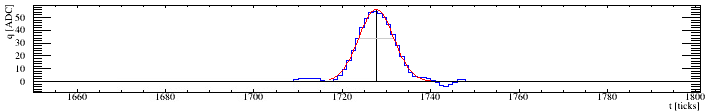
\includegraphics[width = \largefigwidth]{figures-chap4/good_gauss_fit.png}
    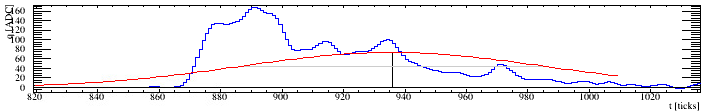
\includegraphics[width = \largefigwidth]{figures-chap4/bad_gauss_fit.png}
    \caption[Example of a well and poorly fitted waveform.]{Waveforms (blue) that have been fitted with a Gaussian (red) from the \textit{GausHitFinder}. Top: an example of a waveform that is well represented by a Gaussian. Bottom: an example of a waveform that is not well represented by a Gaussian.}
    \label{fig:fitted_waveforms}
\end{figure}

\section{Overview of Shower Energy Reconstruction in SBND}\label{subchap:shower reco overview}

Currently, there are three algorithms available for reconstructing \gls{em} shower energy within \gls{sbnd} as part of the \textit{LArPandoraShower} suite of tools, each of which is described below. Regardless of the algorithm used, the initial approach is the same for all three methods which is as follows,
\begin{enumerate}
    \item Identify the hits associated with a given wire plane.
    \item Integrate the hits to obtain the associated charge in \gls{adc} units whilst correcting for electron lifetime. 
    \item Convert the charge in \gls{adc} units to a conventional charge (number of electrons) using the calibration constant which is part of the calorimetry algorithm (this step was not performed in the case of the \textit{Linear Energy tool}). 
\end{enumerate}

Once the charge of a hit has been determined, the final steps which involve converting the charge to energy become method dependent. The other major detector effect that still needs to be considered is recombination, which is modelled by the Modified Box Recombination Model and given by  
\begin{equation}\label{eqn:ModBox}
    \frac{dE}{dx} = \frac{\exp{(\frac{\beta}{\rho \mathcal{E}} W_{ion}.\frac{dQ}{dx}}) - \alpha}{\frac{\beta}{\rho \mathcal{E}}},
\end{equation}
where $\frac{dE}{dx}$ is the deposited energy per unit length, $\frac{dQ}{dx}$ is the deposited charge per unit length,  $\mathcal{E}$ is the electric field in the detector, $\rho$ is the density of liquid argon, $W_{ion} = 23.6$ eV which is the energy required to ionise an argon atom, $\alpha = 0.93 \pm 0.02$ and $\beta = 0.212 \pm 0.002$ (kV/cm)(g/cm$^2$)/MeV. The values for parameters $\alpha$ and $\beta$ are results from the \Gls{argoneut} experiment \cite{ArgoNeuT_recombination_paper}. The recombination correction, \textit{R}, is given by $\frac{\frac{dQ}{dx}.W_{ion}}{\frac{dE}{dx}}$.


Since the recombination model is $\frac{dE}{dx}$ dependent, an accurate path length, \textit{dx}, is needed which requires 3D reconstruction of the direction. Because a shower is treated as a single object, which means the trajectory of constituent components are not tracked, it is therefore not straightforward to directly correct for the recombination effect \cite{MicroBooNE_photon_Ereco_paper}. Two different approaches have been considered and are discussed in the relevant energy reconstruction methods below: 1) assume a nominal recombination value for all hits and 2) use a lookup curve which relates the collected charge to energy which circumvents the need to evaluate a recombination correction directly because it already gets accounted for in the curve.

In the analysis and validation of the shower reconstruction, a number of \textit{true} and \textit{reconstructed} quantities are considered. Care must be taken that it is clear what each value relates to. For clarity, the following quantities are explicitly described;
\begin{itemize}
    \item Collected charge (or energy): This is the charge that is seen by the wire planes. 
    \item Deposited charge (or energy): This is the charge that is initially deposited in the detector. Typically this would be obtained from the collected charge by correcting for the electron lifetime and the recombination effect.
    \item Hit energy: This is the energy associated with each individual hit. Both true and reconstructed values may be obtained.
    \item Energy of showering particle: This is the energy of the particle which results in the shower which is being investigated. 
\end{itemize}
\subsection{Linear Energy Tool}\label{subchap:Linear Energy Tool}
The first shower energy reconstruction method developed was the \textit{Shower Linear Energy tool}. This tool relies on the linear relationship between the true energy deposited in the detector and the reconstructed charge from \gls{mip} muons. A sample of simulated muons are used as calibration because the $\frac{dE}{dx}$ value for electrons and \Gls{mip} muons are not dissimilar. The relationship between the charge obtained from the hits due to the muons and the energy deposited by the muons is shown in \FigureRef{fig:linear lookup curve}. A linear relationship such as this is comparable to assuming a constant recombination factor. 

%\begin{center}
%    \centering
%    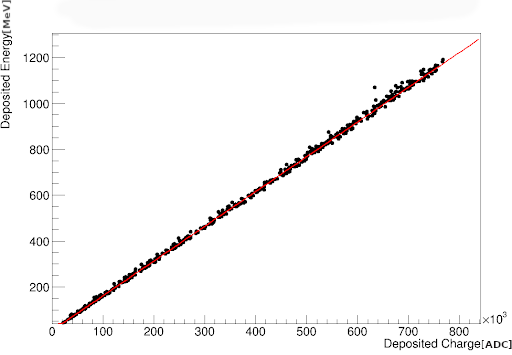
\includegraphics[width = 0.7\textwidth]{figures-chap4/linear_energy_lookup_curve1.png}
%    \captionsetup{type=figure}
%    \captionof{figure}{The linear relationship between deposited charge and energy. Produced from a sample of muons used for calibrating the \textit{Shower Linear Energy tool.}}
%    \label{fig:linear lookup curve}
%\end{center}

To estimate the reconstructed shower energy, the charge found to be associated with a shower would be used to directly read off the associated energy from the linear calibration. A further recombination correction is not required as it has already been accounted for in the charge-to-energy conversion. It should be noted that along with the recombination correction, hit reconstruction and pattern recognition inefficiencies are also corrected for in the calibration curve.  The \textit{Shower Linear Energy tool} has been largely disfavoured since the development of the two other reconstruction tools. 

\begin{figure}[h!]
    \centering
    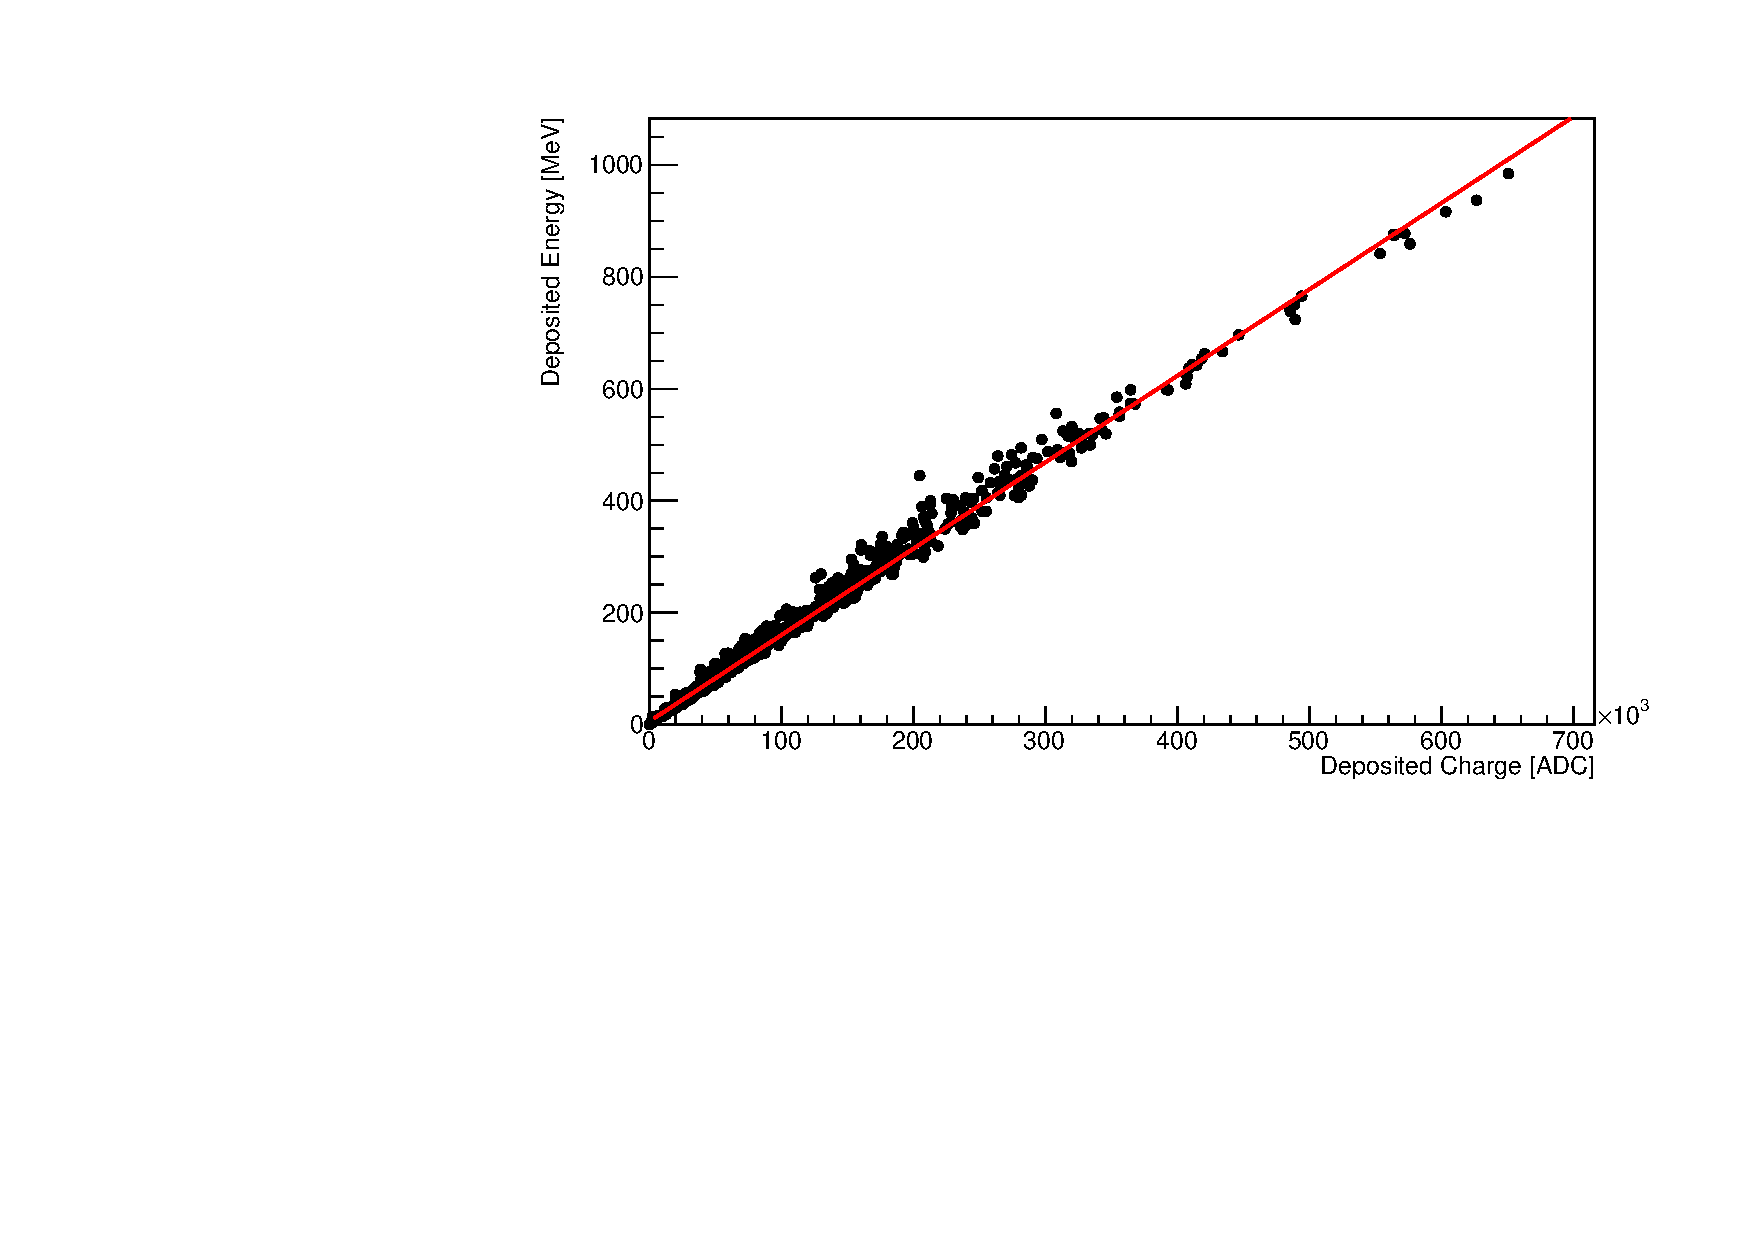
\includegraphics[width = \largefigwidth]{figures-chap4/linear_tool_lookup_curve.pdf}
    \caption{The linear relationship between deposited charge and energy. Produced from a sample of muons used for calibrating the \textit{Shower Linear Energy tool.}}
    \label{fig:linear lookup curve}
\end{figure}

\newpage

\subsection{Number of Electrons to Energy}\label{subchap:kGeVToElectrons}
The \textit{Shower Num Electrons Energy tool} was developed to move away from being reliant on in-house calibration curves and instead use the pre-existing calibration available in the \Gls{sbnd} portion of the \Gls{larsoft} framework. This has the advantage of being much more flexible to physics changes. For example, a change in the recombination correction could be investigated by changing a single number, whereas, for the \textit{Shower Linear Energy tool}, the calibration curves would have to be regenerated. The number of electrons are found from the \gls{adc} charge and are then directly converted to energy using a scale factor which is the inverse of the energy required to ionise an argon atom. A nominal recombination value of 0.64 is assumed which is applied to all hits.

The nominal recombination value was calculated by simulating electrons whilst using a large (effectively infinite) value for the electron lifetime and setting both the transverse and longitudinal diffusion coefficients to zero. The only detector effect remaining that may impact the collected energy is the recombination effect and therefore taking the ratio between the collected and deposited energy will give a value for the recombination effect. For electrons, it was found that the recombination effect was fairly constant at a value of 0.64 across a broad range of energies \cite{recombination_0.64}. 

\begin{comment}

An attempt to correct for the \Gls{sce} can be made with this method by utilising the Modified Box Recombination Model which is given by \begin{equation}\label{eqn:ModBox}
    \frac{dE}{dx} = \frac{\exp{(\frac{\beta}{\rho \mathcal{E}} W_{ion}.\frac{dQ}{dx}}) - \alpha}{\frac{\beta}{\rho \mathcal{E}}}
\end{equation}
where $\frac{dE}{dx}$ is the deposited energy per unit length, $\frac{dQ}{dx}$ is the deposited charge per unit length,  $\mathcal{E}$ is the electric field in the detector, $\rho$ is the density of liquid argon, $W_{ion} = 23.6$ eV which is the energy required to ionise an argon atom, $\alpha = 0.93 \pm 0.02$ and $\beta = 0.212 \pm 0.002$ (kV/cm)(g/cm$^2$)/MeV. The values for parameters $\alpha$ and $\beta$ are results from the \Gls{argoneut} experiment \cite{ArgoNeuT_recombination_paper}. The recombination correction, \textit{R} is given by $\frac{\frac{dQ}{dx}.W_{ion}}{\frac{dE}{dx}}$ and by taking the nominal values of \textit{R} and $\mathcal{E}$ a nominal value for $\frac{dE}{dx}$ is calculated using \EquationRef{eqn:ModBox}. Assuming the nominal value of $\frac{dE}{dx}$ is constant, \textit{R} may be expressed as $R = R(\mathcal{E}$). For each of the hits, their corresponding \Gls{sp} are found and the coordinates of the \Gls{sp} in the detector are determined. Instead of using the nominal value for $\mathcal{E}$, the local value for $\mathcal{E}$ at the position of the \Gls{sp} is used and the corresponding value for \textit{R} is calculated. The method to estimate the reconstructed energy is the same as the case without any \Gls{sce} corrections except the modified value for \textit{R} is used. In the case that a hit has no corresponding \Gls{sp}, the charge weighted centre of the shower is found and the local value of $\mathcal{E}$ at this point is used instead.

\begin{figure}[h]
    \centering
    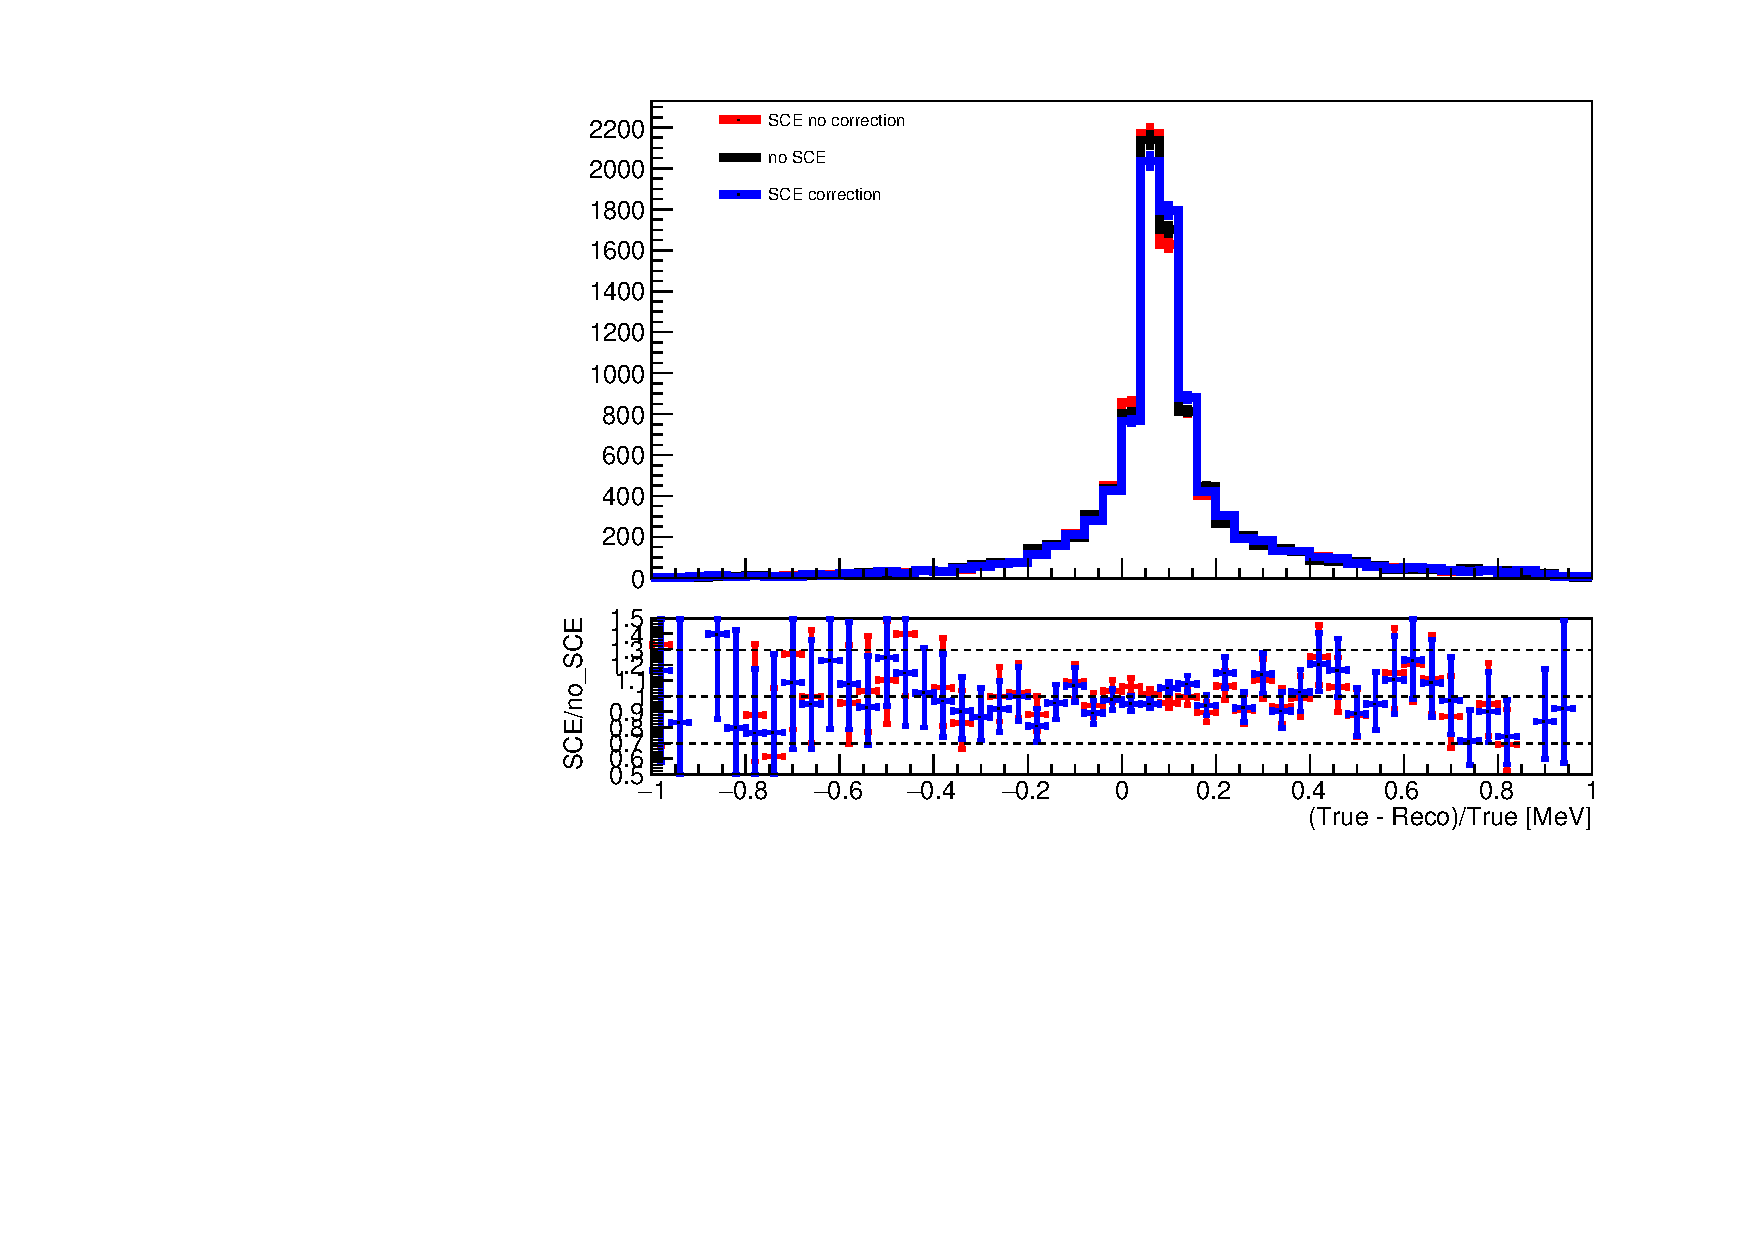
\includegraphics[width = \largefigwidth]{figures-chap4/ratio_plot_oldmethod_trueshoweringparticle.pdf}
    \caption{Caption}
\end{figure}



Shortcoming (don't know how much to put here? don't know if i want to emphasise how bad stuff is..): 
\begin{itemize}
    \item Things revolve around the nominal recomb of 0.64 - not really that realistic. 
    \item Correcting for SCE 'properly' is not straightforward either - using a fixed nominal dE/dx isn't ideal.
\end{itemize}

\end{comment}

\subsection{ESTAR Method}
The \textit{Shower ESTAR Energy tool} combines the ESTAR database provided by the \gls{nist} along with the Modified Box recombination model in an approach that was first used by the \Gls{argoneut} experiment \cite{ArgoNeuT_ESTAR_paper}. The ESTAR database provides the track length of electrons in various materials, including liquid argon, for energies ranging from 0.01 MeV to 1000 MeV \cite{ESTAR_Database}.

$\frac{dE}{dx}$ values may be calculated by dividing the energy by the track length for each entry in the ESTAR database. The deposited charge, \textit{Q}, can then be found by using \EquationRef{eqn:ModBox} to find $\frac{dQ}{dx}$ and multiplying by the track length, \textit{dx}. This now allows the collected charge and energy to be related. If $\mathcal{E}$ in \EquationRef{eqn:ModBox} is taken to be a variable, the above process may be repeated whilst iterating over a set value of $\mathcal{E}$. This results in a 3D curve relating both the deposited charge and electric field to energy as is shown in \FigureRef{fig:ESTAR lookup curve}. The energy may then be interpolated from the collected charge and the appropriate electric field. As with the \textit{Shower Linear Energy tool}, a direct correction for recombination is not needed as it is again accounted for in the lookup curve. 

\begin{figure}[h!]
    \centering
    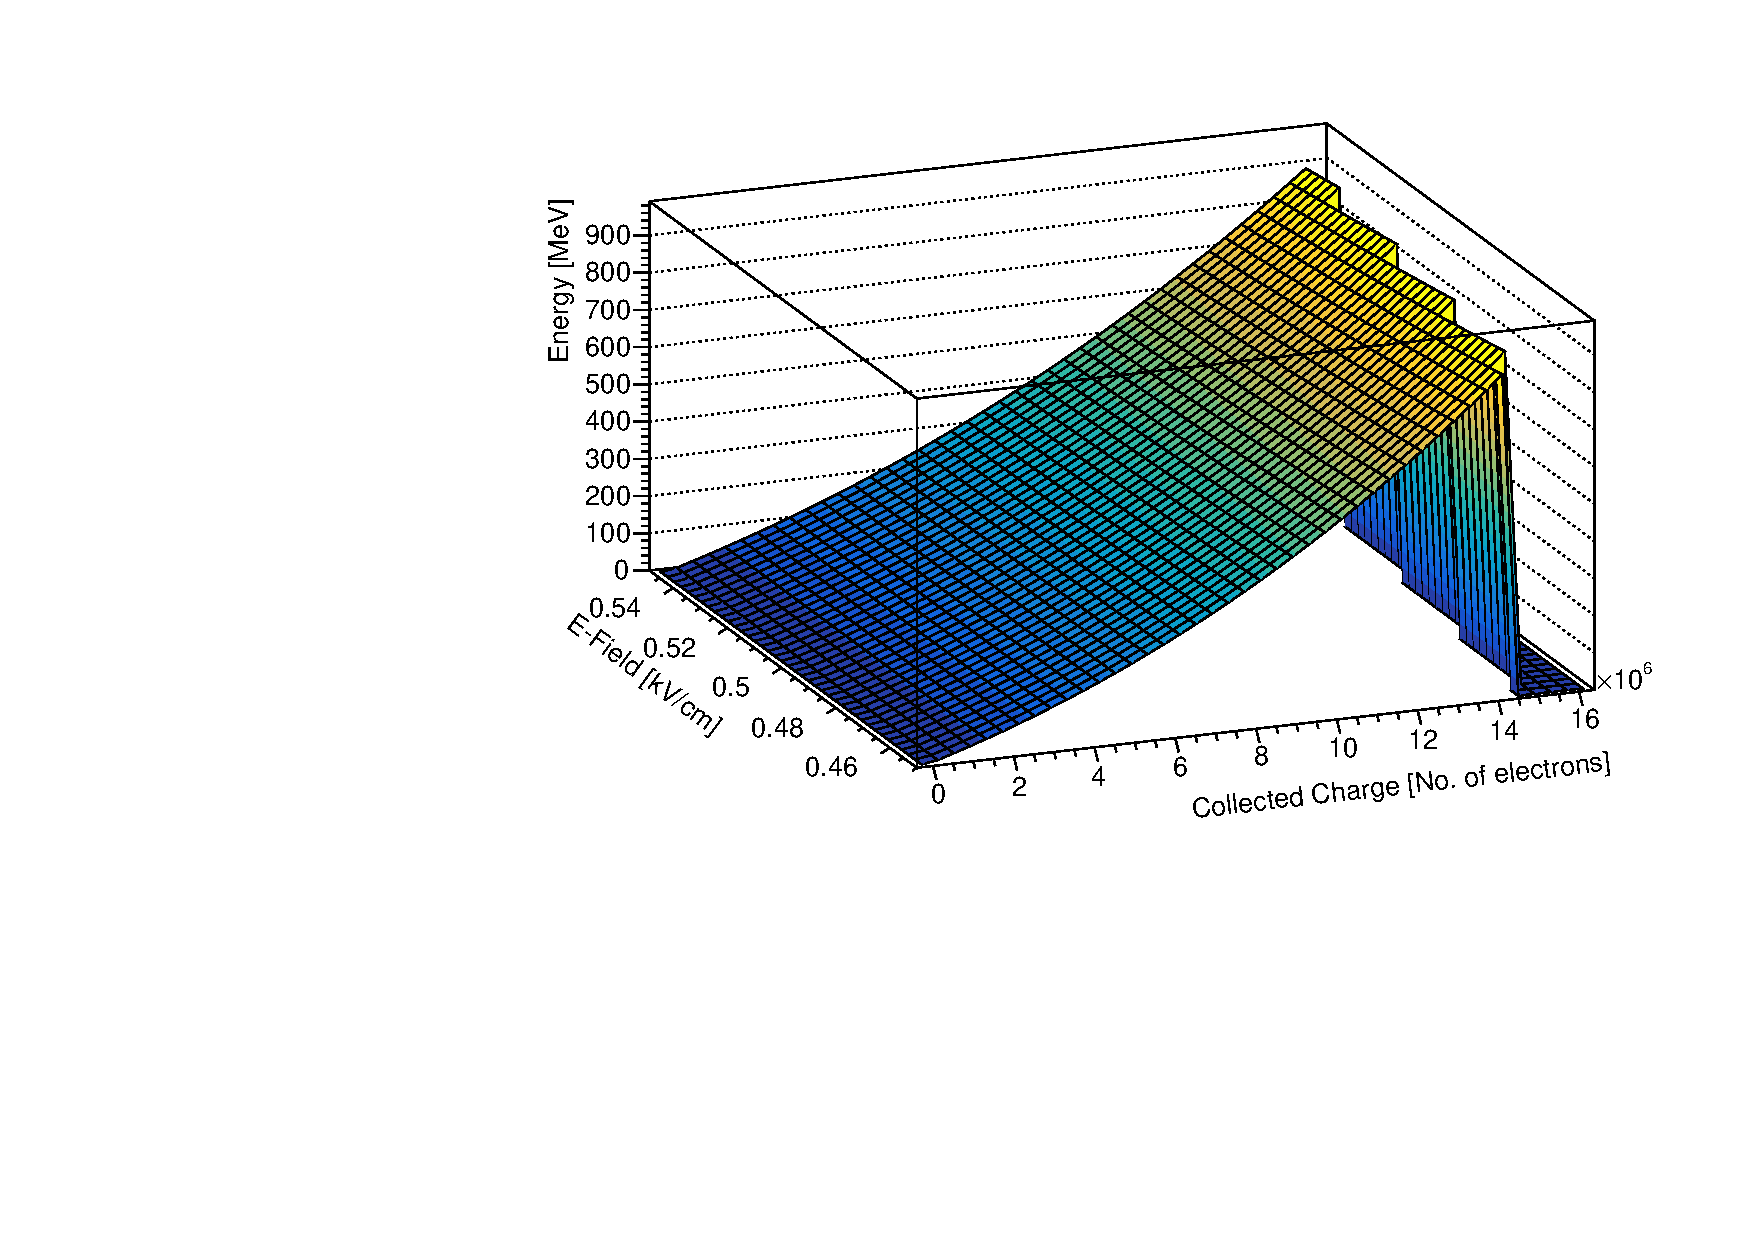
\includegraphics[width = 0.8\textwidth]{figures-chap4/ESTAR_lookup_curve.pdf}
    \caption[ESTAR lookup curve.]{ESTAR lookup curve generated from the ESTAR database and the Modified Box Recombination Model.}
    \label{fig:ESTAR lookup curve}
\end{figure}

\newpage
\section{Shower Energy Reconstruction Performance}

In order to assess the performance of the different reconstruction methods, a comparison with \textit{truth} information is performed. Depending on the approach, a few other inefficiencies should be considered, namely that the hit reconstruction and Pandora pattern recognition are not perfect \cite{Pandora_paper}. This results in hits missing due to not being reconstructed plus the addition of the clusters that Pandora produces being incomplete. Therefore, there are typically fewer hits than there would be if the shower in question were to be perfectly reconstructed. Reconstructing the energy of the showering particle, is desirable for a number of analyses, however, due to these issues, it is not realistic to expect agreement to be within a few per cent. Improving the hit reconstruction or the pattern recognition within Pandora would clearly help, but it is likely that a non-negligible bias would remain. Work on Pandora, the hit reconstruction and addressing any remaining bias is however beyond the scope of this chapter. To circumvent the inefficiencies in Pandora's pattern recognition, Pandora is run in \textit{cheating} mode, which means that truth information is used to perform the clustering. This decouples the reconstruction methods from any effects due to Pandora's pattern recognition. For comparison, a number of figures showing the reconstruction performance without using Pandora in cheating mode are shown in \AppendixRef{app:reconstruction_performance}.

To purely gauge the performance of a given reconstruction method, it is probably best to compare the truth and reconstructed energy of a shower by only considering the available hits. This way, the reconstruction method is only validated from the available information and is additionally decoupled from hit reconstruction inefficiencies. However, additional care must be taken when using the true energy of the hits. What is considered a hit is user defined in that the width that defines a hit is a parameter that may be changed. Therefore, the true energy associated with a hit is dependent on the chosen width. Within \gls{larsoft}, the default width of a hit is $1\sigma$ which is chosen to try and find a balance between covering a sufficient amount of charge whilst still being able to resolve multiple hits which are closely spaced. The hit width considered here has been left at the default value of $1\sigma$. 

Generally, the validation is performed on a shower-hit level. This means that for a given shower, the energy of each hit is reconstructed and then summed together to obtain the energy of the shower. The exception to this is in the case of the \textit{Linear Energy tool}. During its development, it was customary to sum up the charge of all the hits and then convert to energy. This is why the calibration curve in \FigureRef{fig:linear lookup curve} has energies on the order of a shower level and not a hit level (individual hit energies are usually $\lesssim 5$ MeV) and also why it is possible to evaluate shower energies above 1000 MeV using the ESTAR method. 

\subsection{Validation of a BNB Sample}

In order to validate the reconstruction methods, an $e^- + \pi^+$ vertex sample with \gls{bnb}-like properties was produced where the electron is the showering particle. The pattern recognition is comprised of a number of steps some of which rely on the reconstructed vertex. It is therefore important to correctly reconstruct the vertex to avoid inaccuracies in the pattern recognition and it is usually easier to accurately reconstruct the vertex of an event if two particles are emanating from a single point rather than just one particle. Unless otherwise stated, all the validation has been performed using the collection plane. 

The true vs reconstructed energy is shown in \FigureRef{fig:reco_vs_true_hit_level} for all three methods where the true energy has been calculated from the shower hits. The results from the \textit{Shower Linear Energy tool} and the \textit{Shower ESTAR Energy tool} are similar and show good agreement between true and reconstructed energies across the whole energy range whereas the \textit{Shower Num Electrons Energy tool} tends to overestimate the hit energies. \FigureRef{fig:reco_vs_true_showeringE} is similar, but instead, the true energy is the energy of the showering electron. This gives a measure of the bias each method can expect due to the inefficiencies mentioned above. Both the \textit{Shower Linear Energy tool} and the \textit{Shower ESTAR Energy tool} underestimate the true energy of the showering electron as is expected. The \textit{Shower Num Electrons Energy tool} shows better agreement due to systematically applying a higher energy to individual hits which compensates for other inefficiencies. 

\begin{figure}[h!]
    \centering
    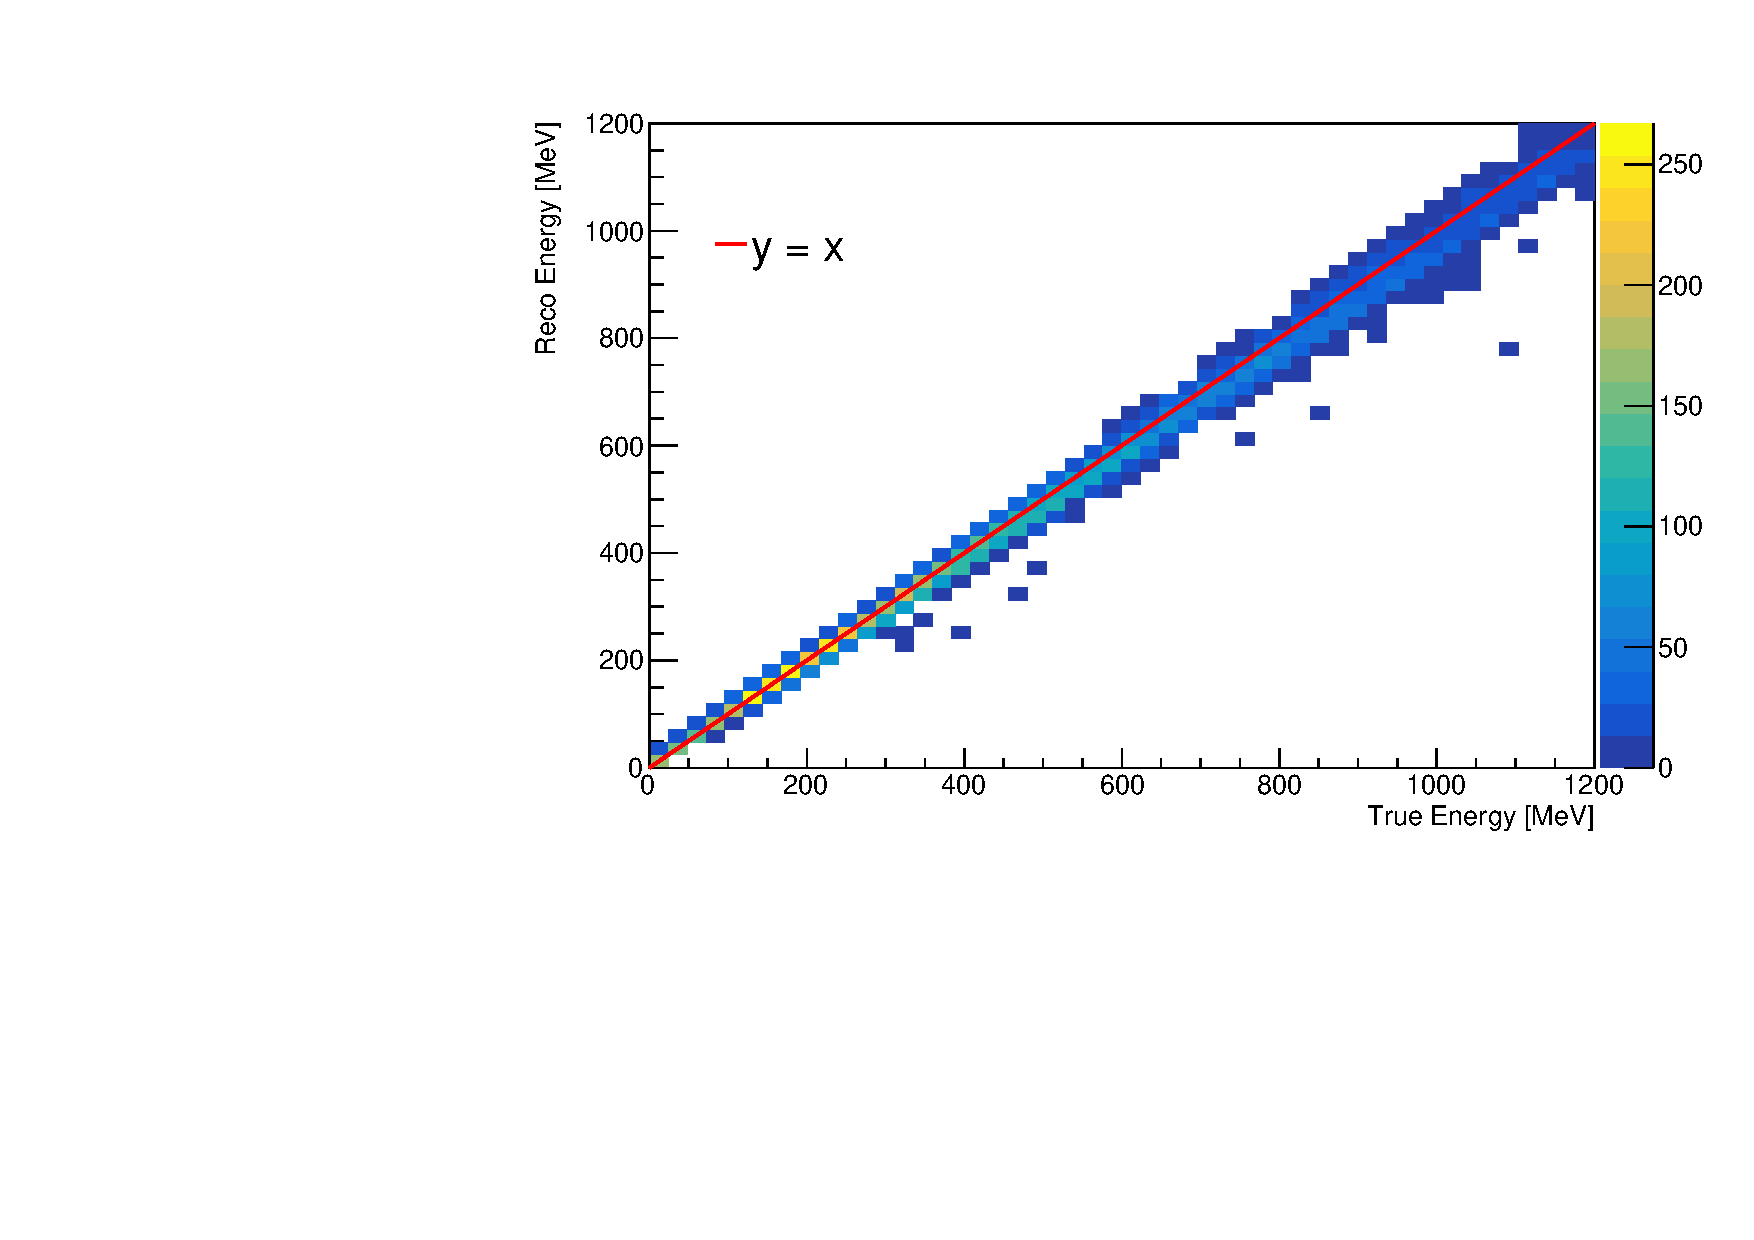
\includegraphics[width = 0.49\textwidth]{figures-chap4/true_vs_reco_linear.pdf}
    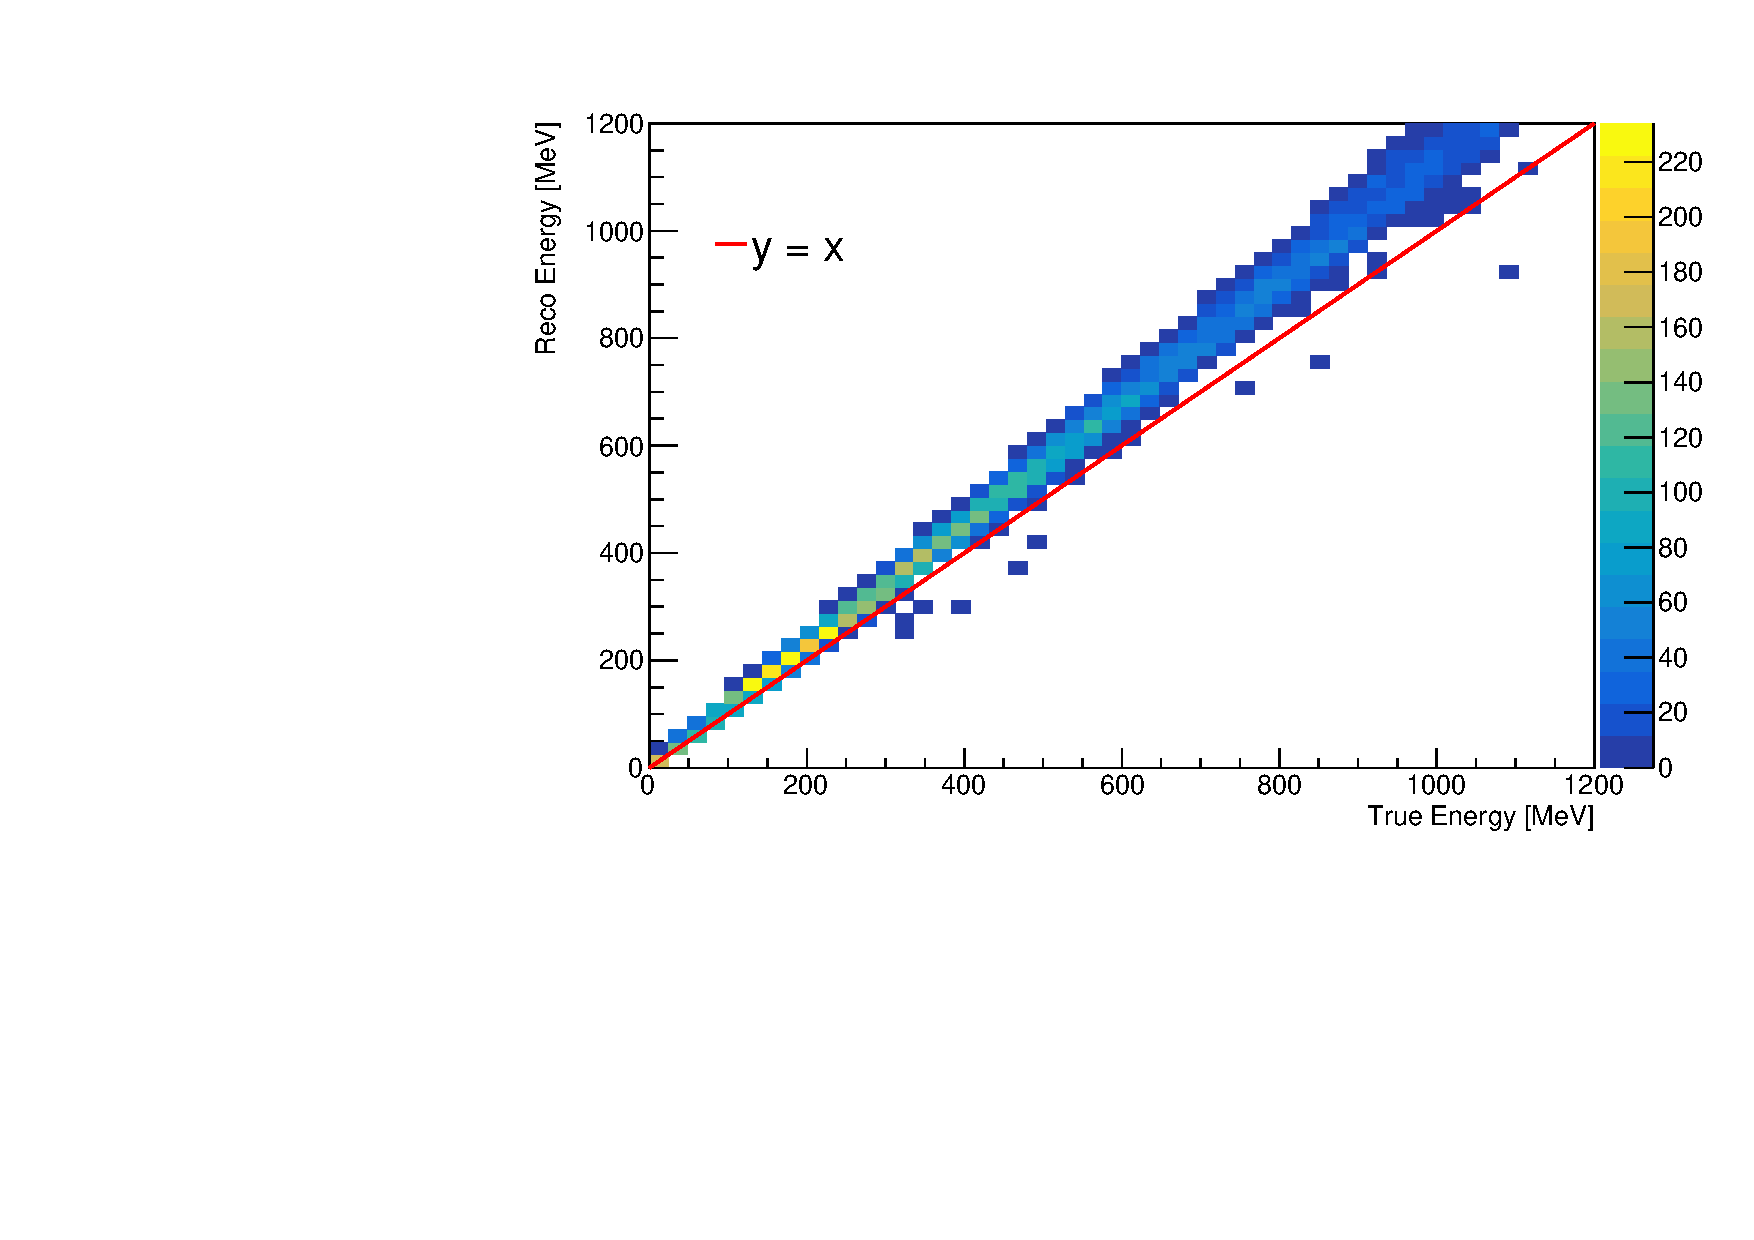
\includegraphics[width = 0.49\textwidth]{figures-chap4/true_vs_reco_oldmethod.pdf}
    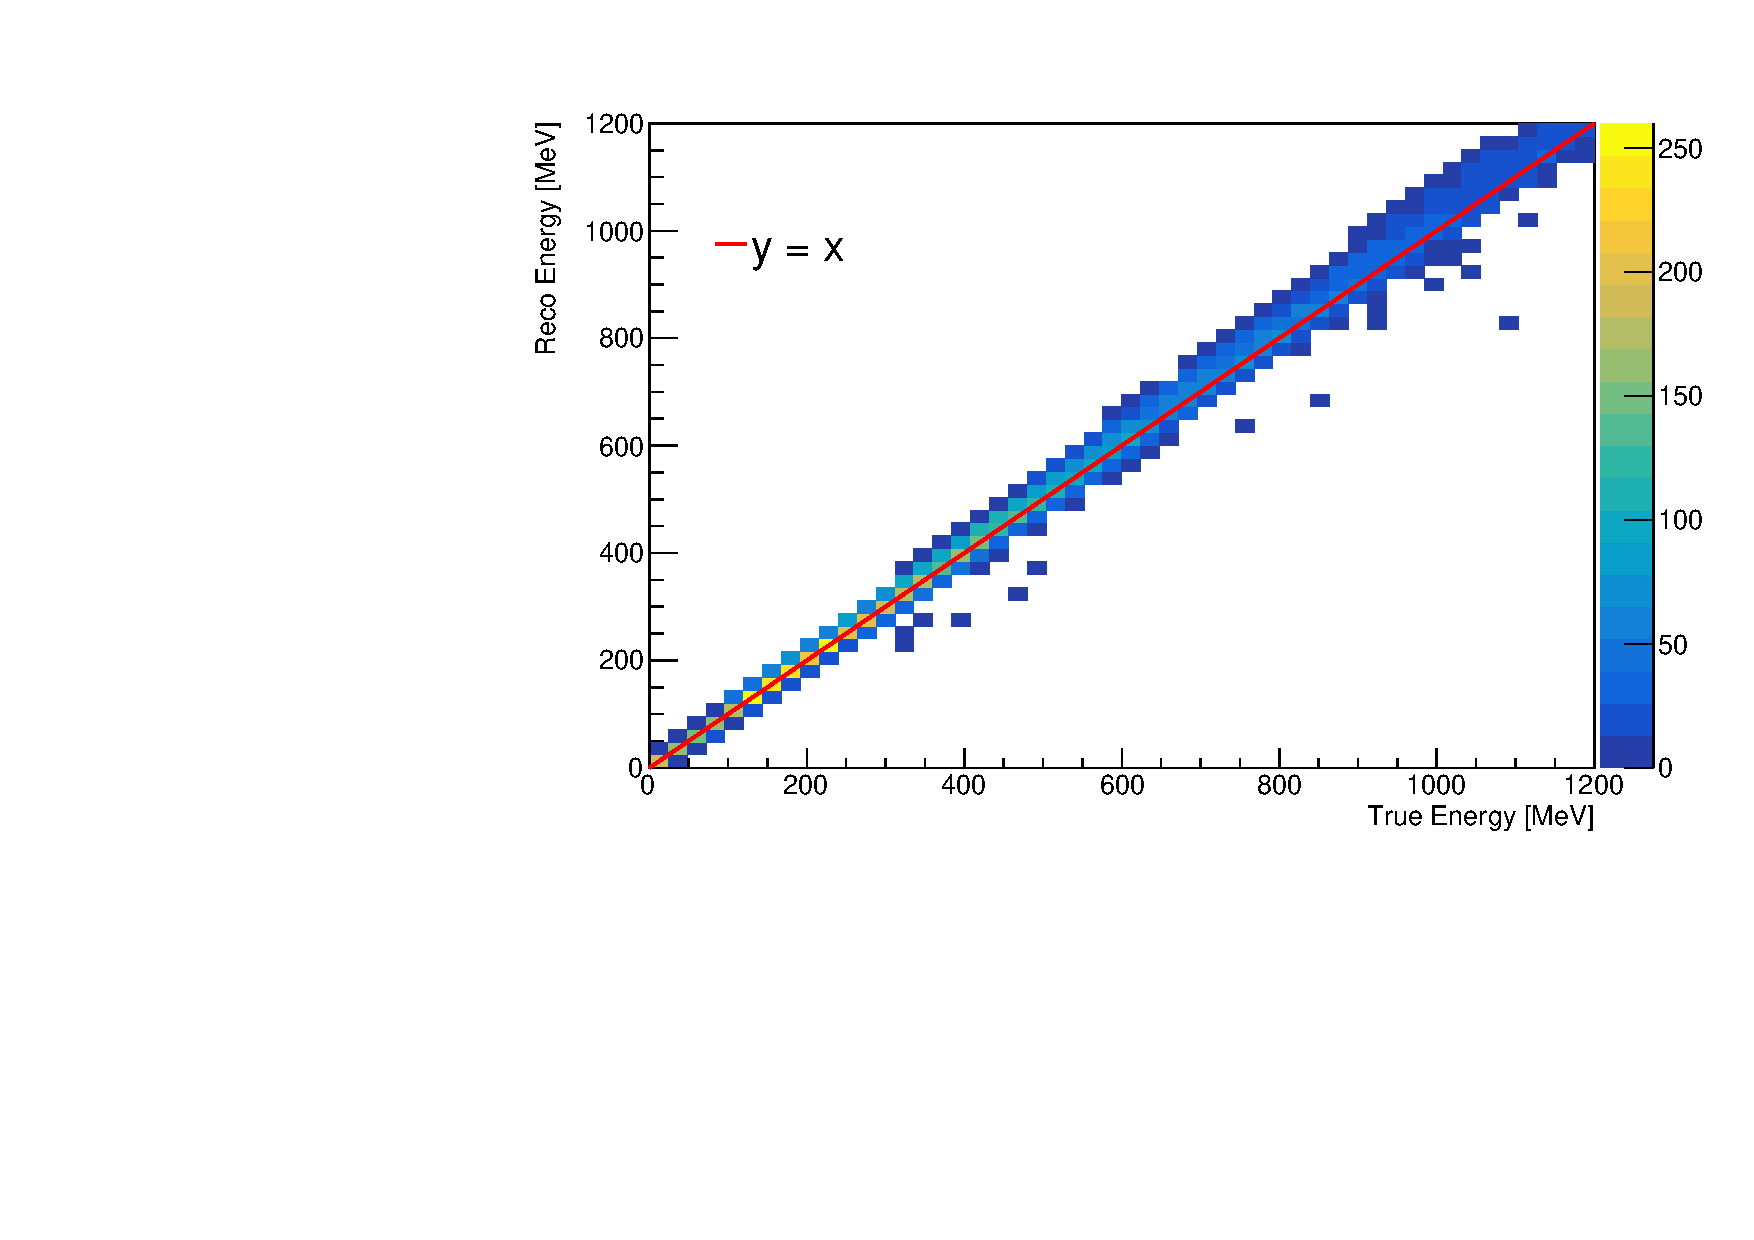
\includegraphics[width = 0.49\textwidth]{figures-chap4/true_vs_reco_ESTAR.pdf}
    \captionsetup{width=0.45\textwidth}
    \parbox[b]{0.49\textwidth}%
  {
    \caption[True vs reconstructed energy from a showering electron. The true energy has been evaluated from the hits of each shower.]
    {True vs reconstructed energy from a showering electron. The true energy has been evaluated from the hits of each shower. Top Left: \textit{Shower Linear Energy tool}, Top Right: \textit{Shower Num Electrons Energy tool} and Bottom Left: \textit{Shower ESTAR Energy tool}. \\}
    \label{fig:reco_vs_true_hit_level}}
\end{figure}


\begin{figure}[h!]
    \centering
    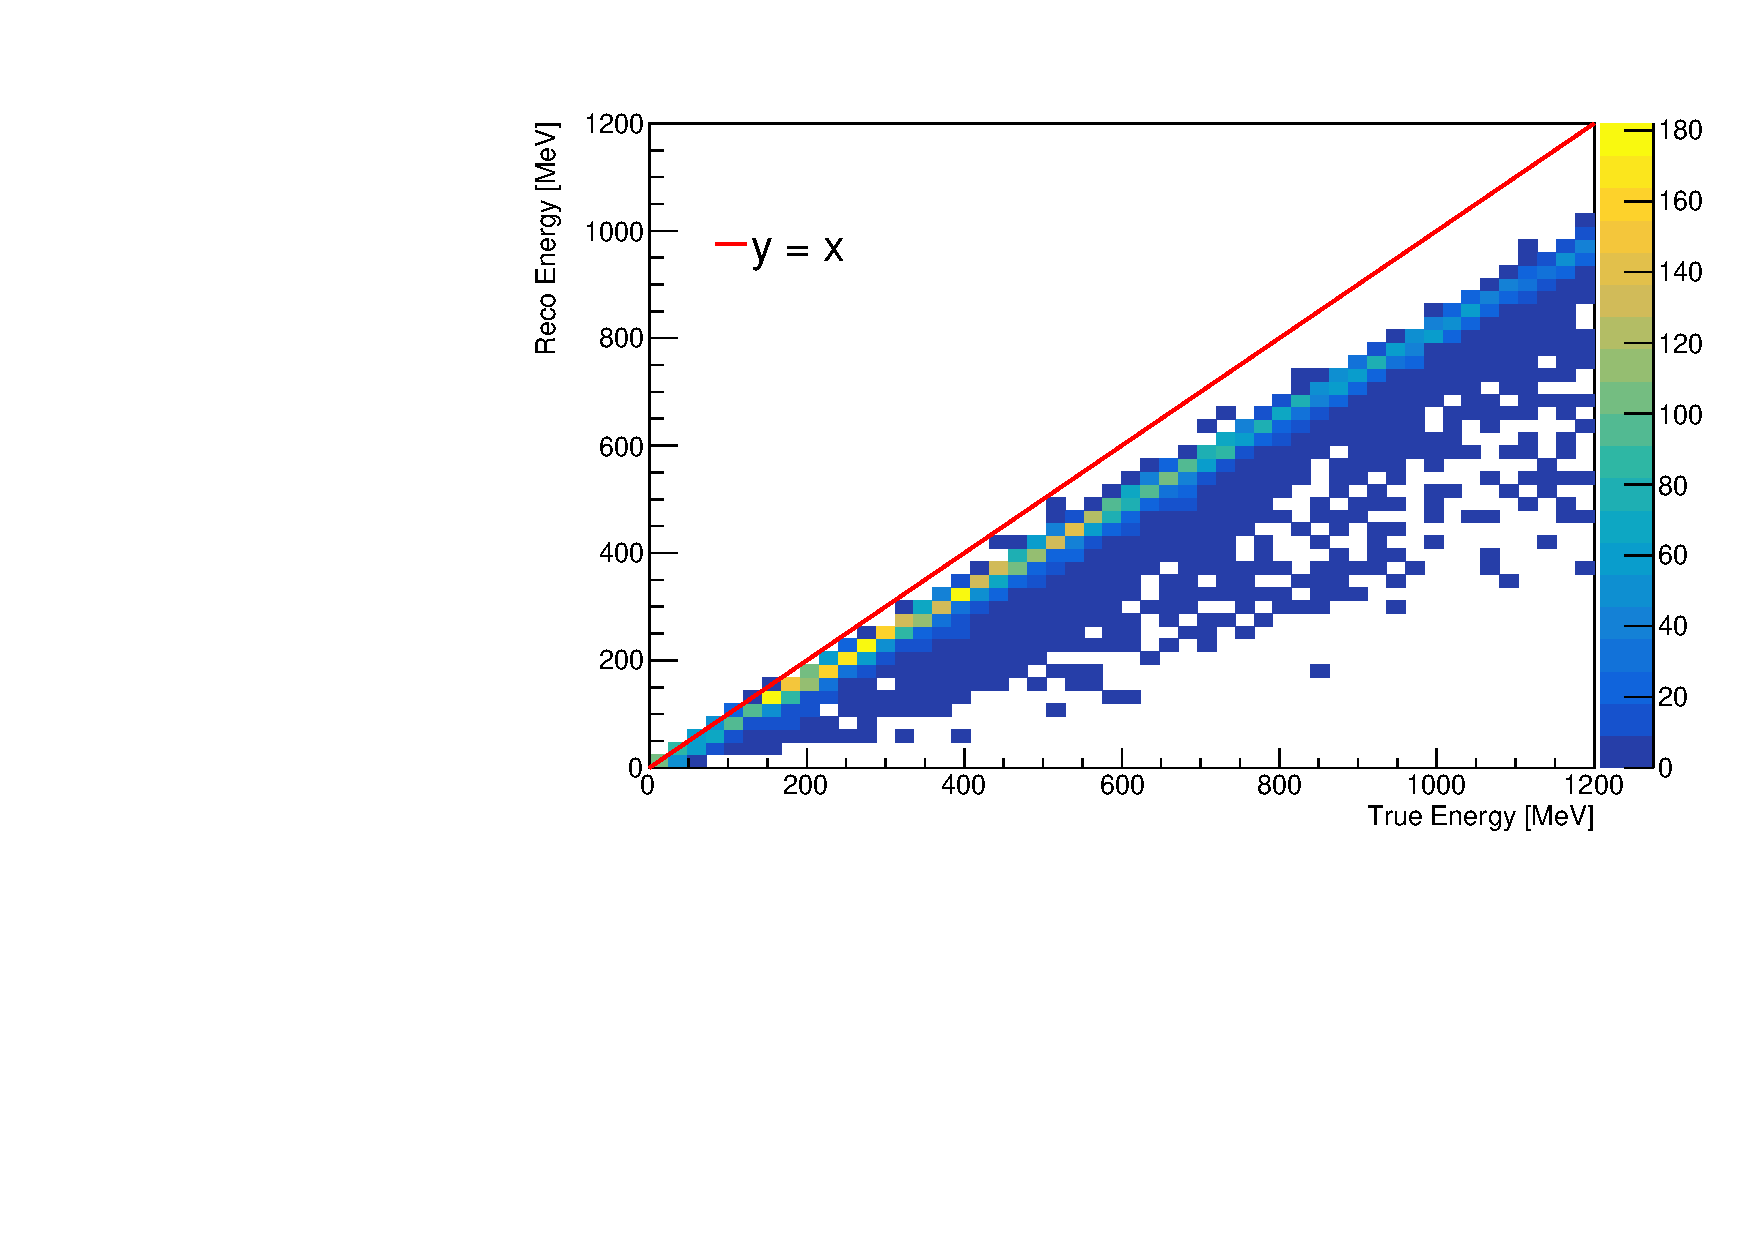
\includegraphics[width = 0.49\textwidth]{figures-chap4/true_vs_reco_showeringE_linear.pdf}
    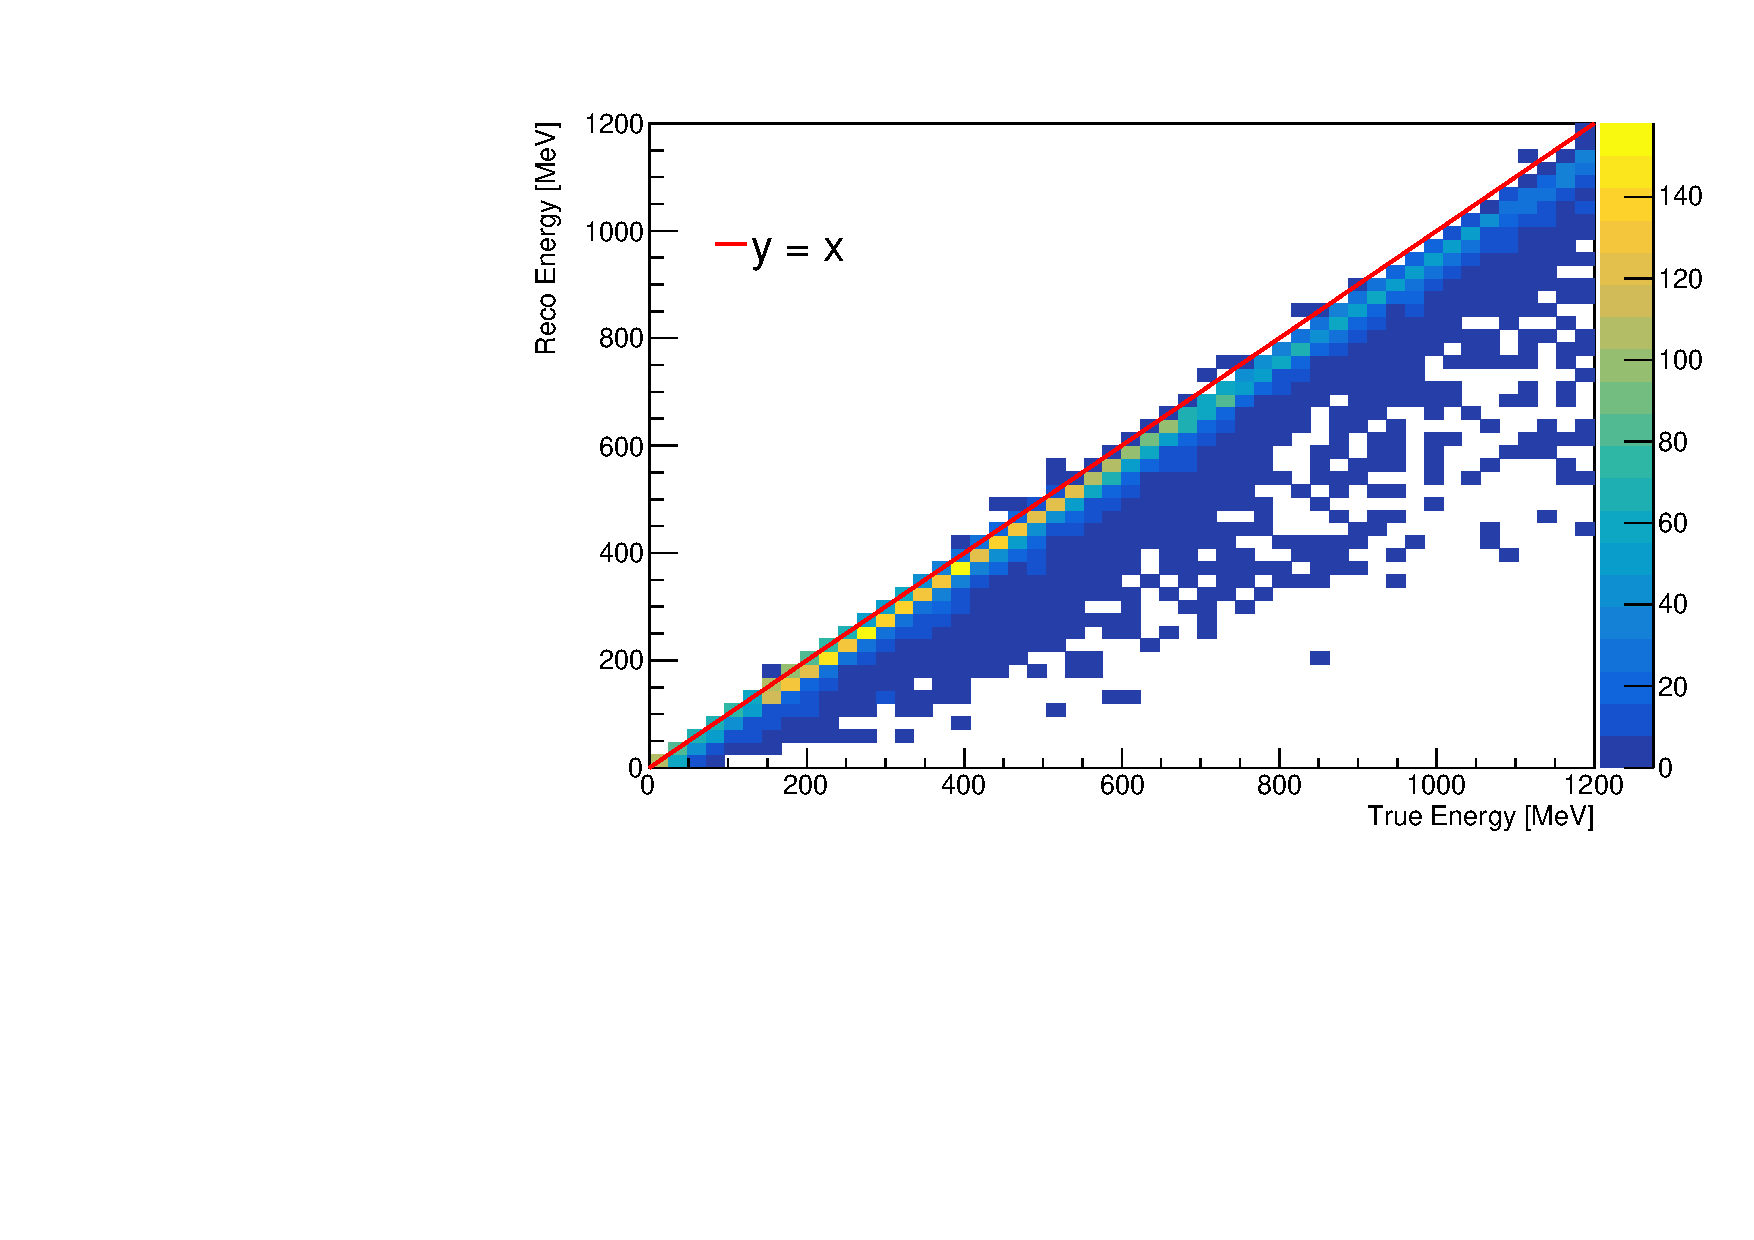
\includegraphics[width = 0.49\textwidth]{figures-chap4/true_vs_reco_showeringE_oldmethod.pdf}
    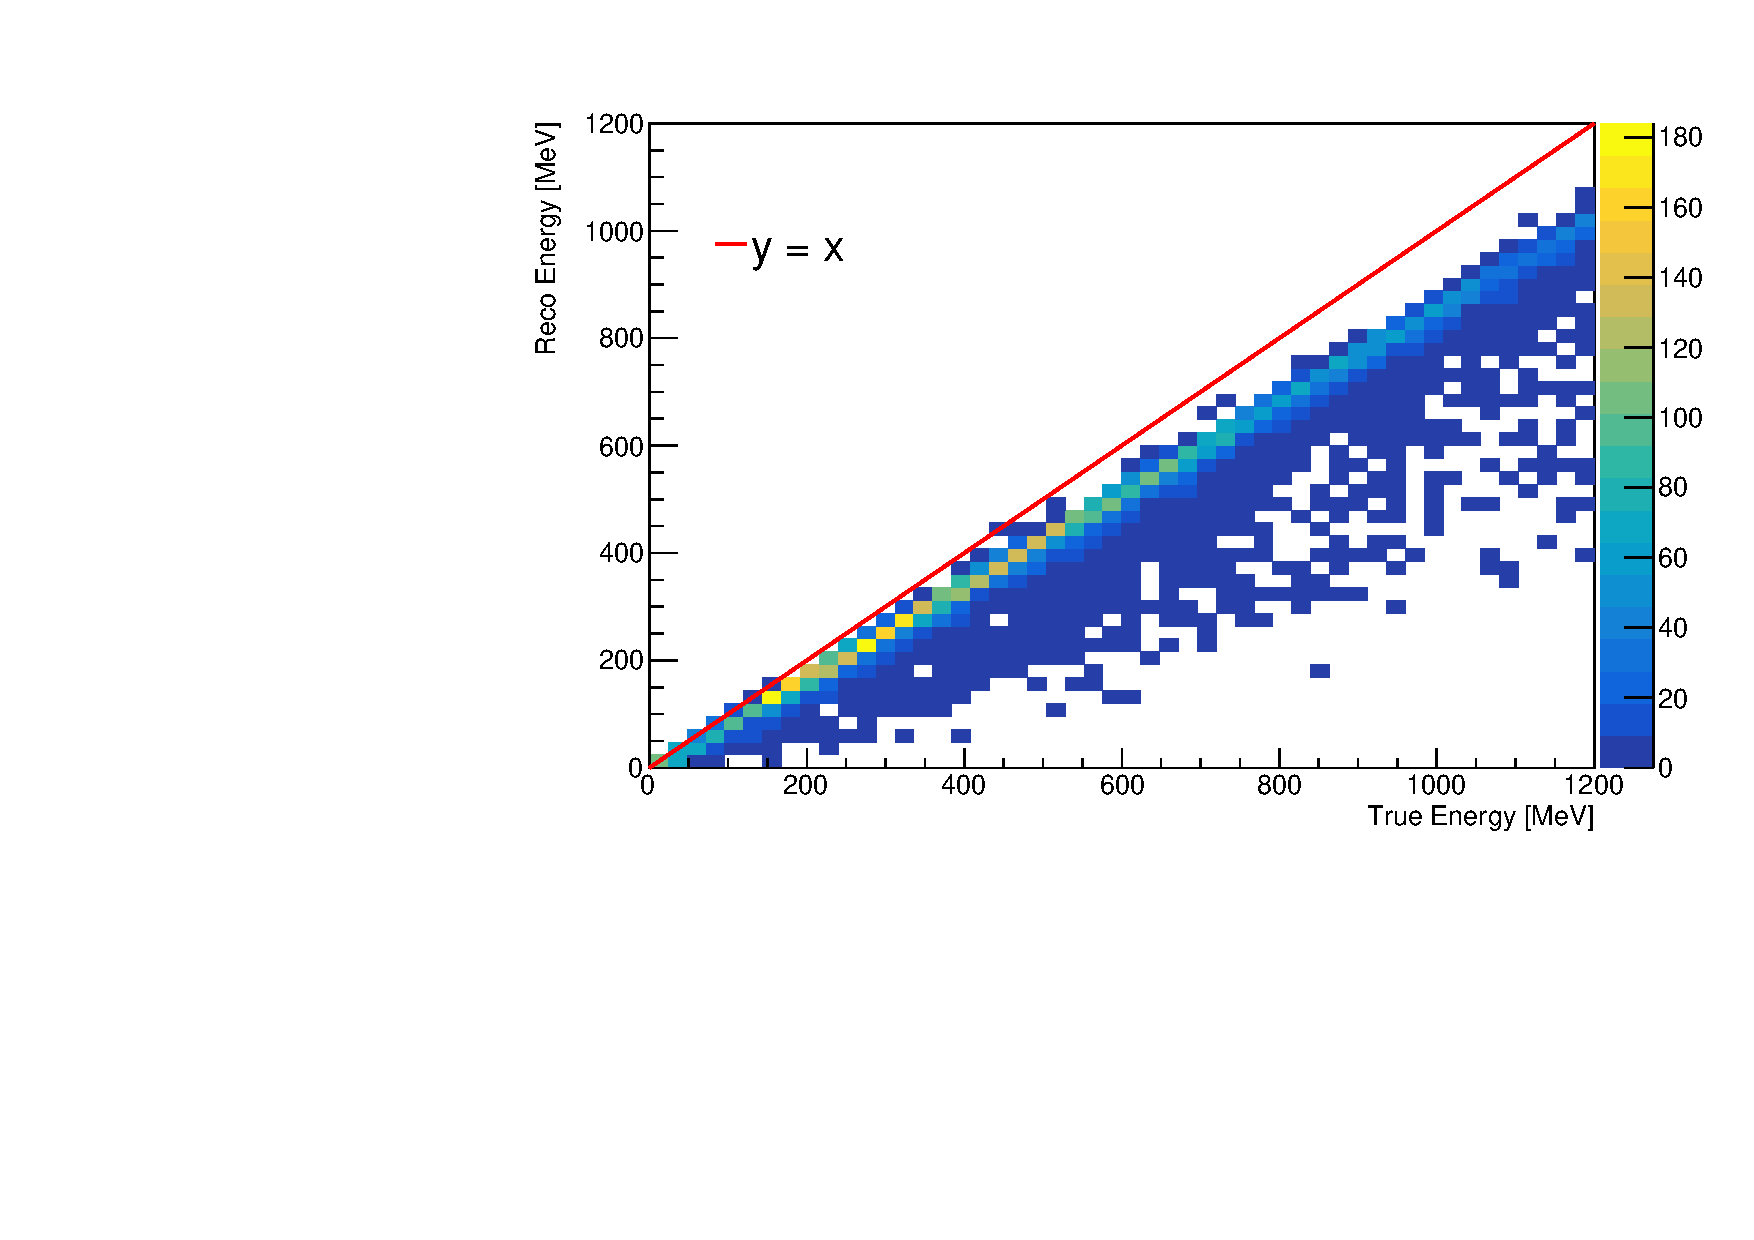
\includegraphics[width = 0.49\textwidth]{figures-chap4/true_vs_reco_showeringE_ESTAR.pdf}
    \captionsetup{width=0.45\textwidth}
    \parbox[b]{0.49\textwidth}%
  {
    \caption[True vs reconstructed energy from a showering electron. The true energy is the energy of the showering electron.]
    {True vs reconstructed energy from a showering electron. The true energy is the energy of the showering electron. Top Left: \textit{Shower Linear Energy tool}, Top Right: \textit{Shower Num Electrons Energy tool} and Bottom Left: \textit{Shower ESTAR Energy tool}. \\}
    \label{fig:reco_vs_true_showeringE}}
\end{figure}

\newpage
A comparison of the fractional energy separation, which is defined as $\frac{Reco - True}{True}$, is shown in \FigureRef{fig:fractional_energy_resolution} for both true energies. When comparing with the true energy of the hits, the \textit{Shower ESTAR Energy tool} peaks quite tightly around zero as does the \textit{Shower Linear Energy tool}. The \textit{Shower Num Electron Energy tool} peaks to the right of the zero line again indicating that the reconstructed quantity is an overestimate. All three distributions peak to the left of the zero line when compared with the true energy of the showering particle with the \textit{Shower Num Electrons Energy tool} giving the closest result. 



\begin{figure}[h!]
    \centering
    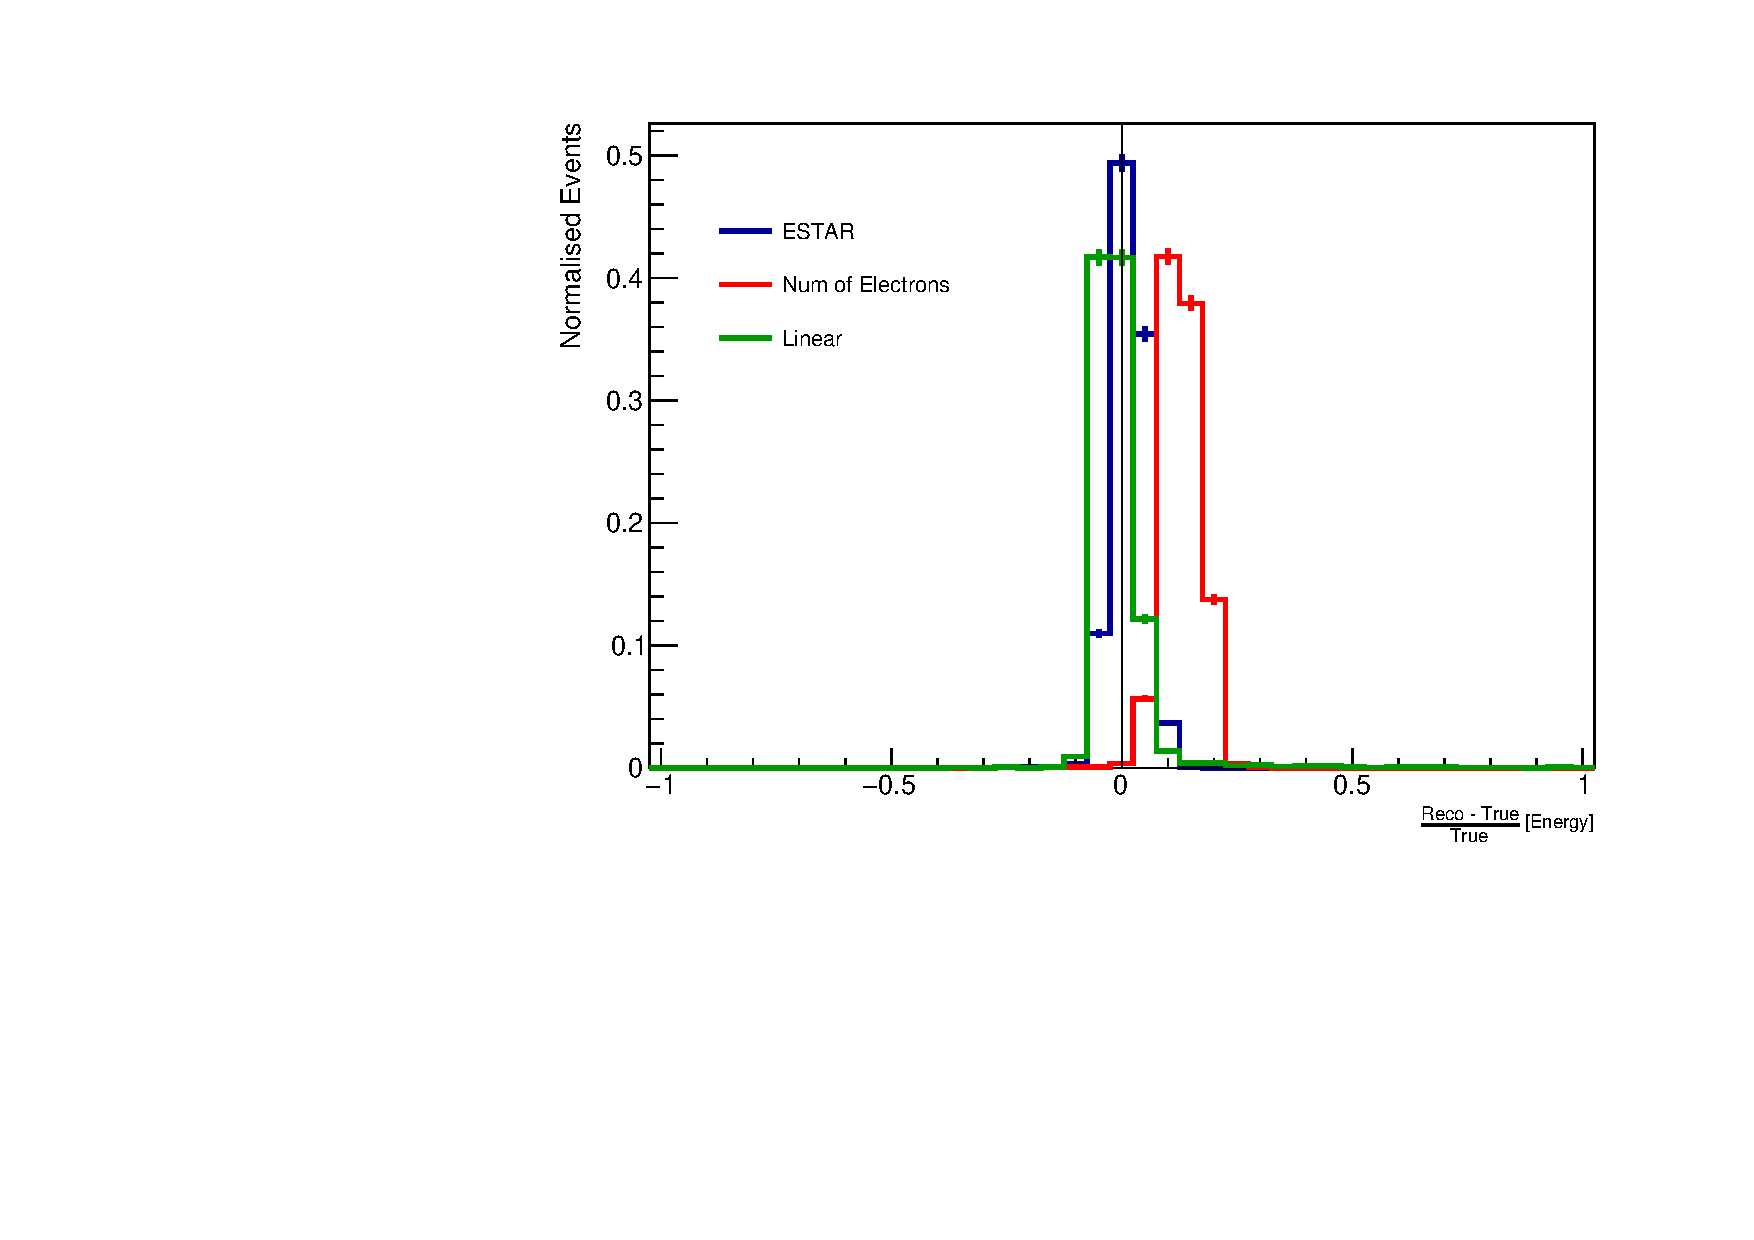
\includegraphics[width = 0.49\textwidth]{figures-chap4/bias_cheat_plane_2_all.pdf}
    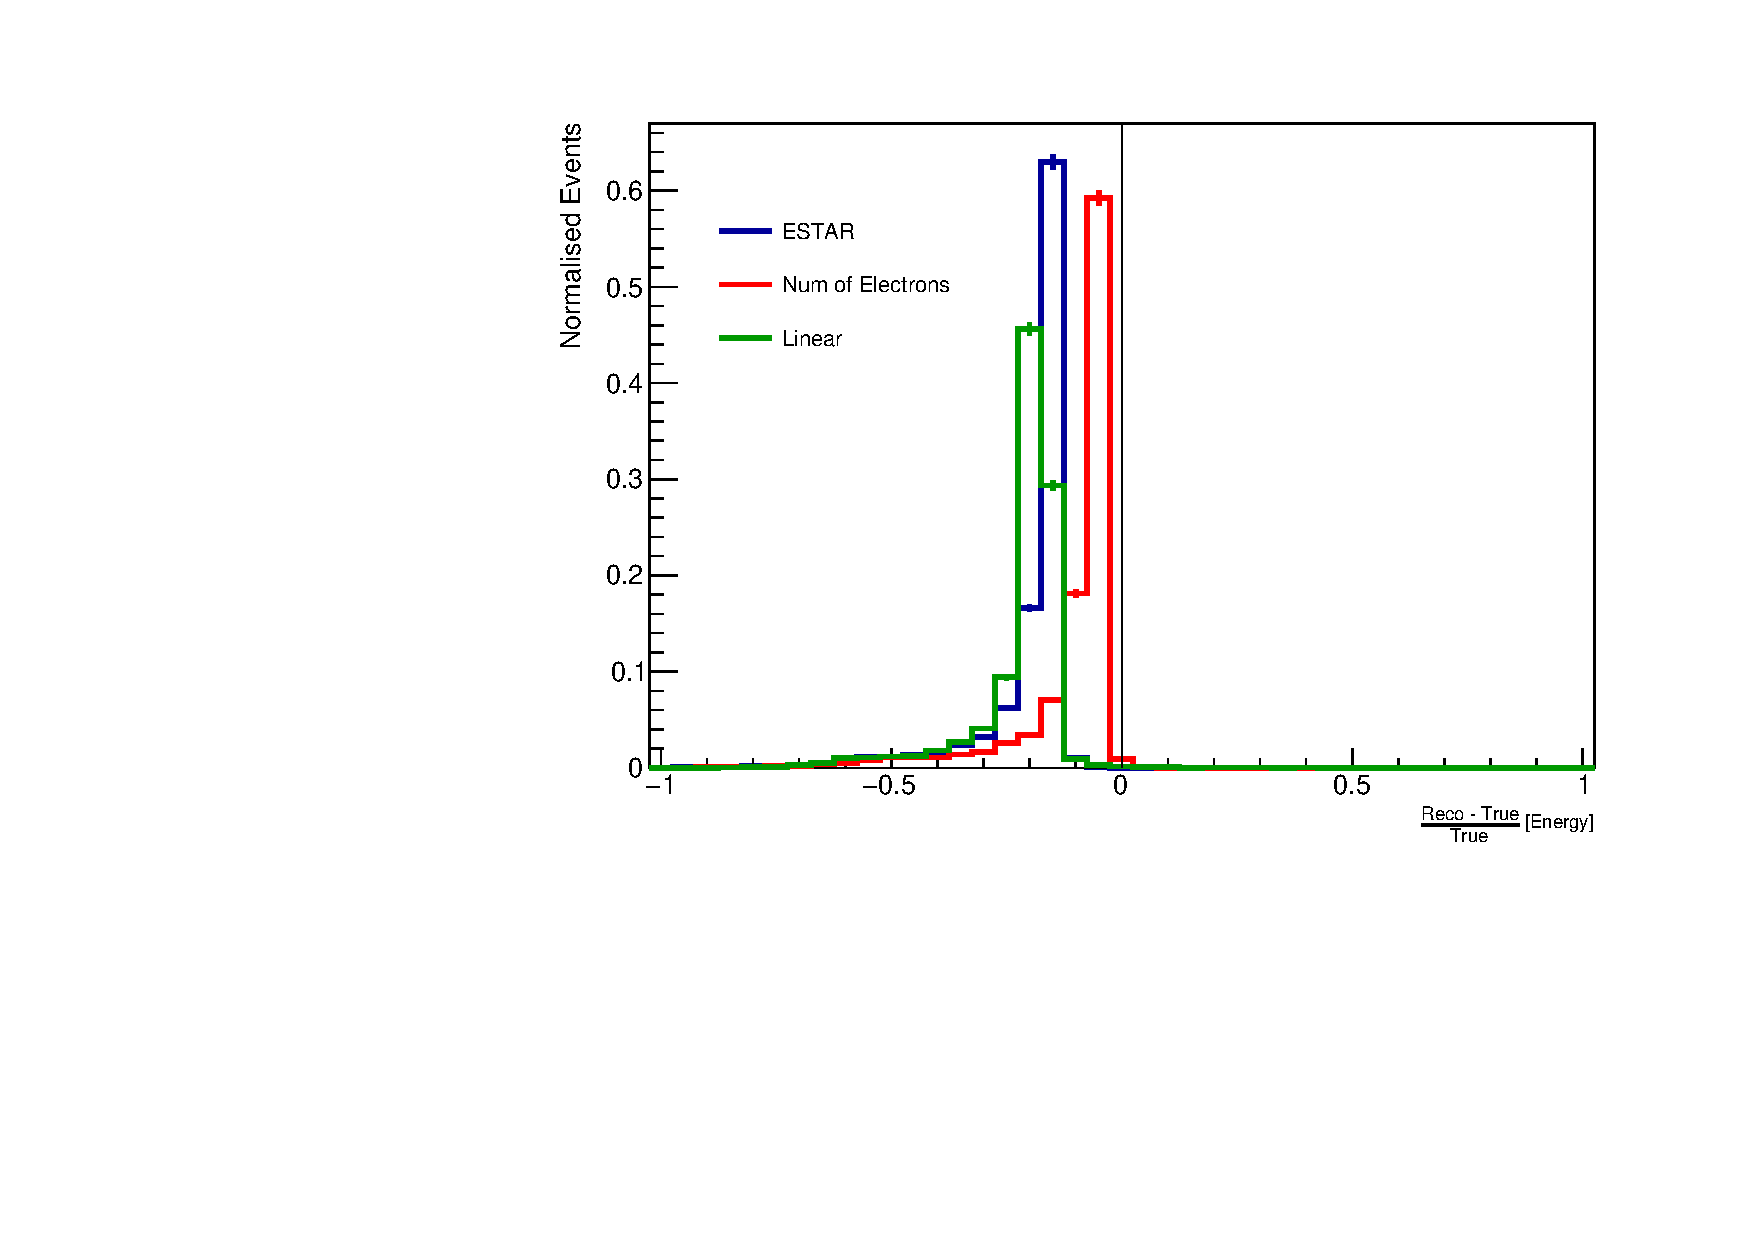
\includegraphics[width = 0.49\textwidth]{figures-chap4/bias_cheat_plane_2_all_showeringE.pdf}
    \caption[Comparison of the fractional shower energy separation.]{Comparison of the fractional shower energy separation for the \textit{Shower Linear Energy tool}, the \textit{Shower Num Electrons Energy tool} and the \textit{Shower ESTAR Energy tool}. Left: Using the true energy of the hits. Right: Using the true energy of the showering particle.}
    \label{fig:fractional_energy_resolution}
\end{figure}

\newpage
To get a measure of the resolution, which is defined as the width of the distribution, a Gaussian of the form 
\begin{equation}
    A \exp{\left(-0.5\left(\frac{x - \mu}{\sigma}\right)^2\right)},
\end{equation}
is fitted to each distribution, where \textit{A} is a constant that defines the peak of the Gaussian, $\mu$ is the mean value and $\sigma^2$ is the variance. $\sigma$ is the quantity that defines the width of the Gaussian fit and will therefore also give a measure of the resolution of the associated distribution. For the distributions which use the true energy of the hits (the left plot of \FigureRef{fig:fractional_energy_resolution}), Gaussians are fitted to the entire distribution, whereas for the distributions using the true energy of the showering electron (the right plot of \FigureRef{fig:fractional_energy_resolution}), Gaussians are only fitted to the central region which encompasses the peak of the distribution. The reason for not fitting a Gaussian to the entire distribution in the second case is in order to avoid having the fit be influenced by the non-Gaussian tail which is usually caused by issues in the reconstruction. Since the tail in the first case is minimal, this is not a concern and therefore a fit to the whole distribution is suitable. 

The Gaussian fits to the fractional energy separation distributions of each of the three reconstruction algorithms are shown in \FigureRef{fig:gauss_fit_hit_level} and \FigureRef{fig:gauss_fit_showering_e} for the comparison with the true energy of the hits and the true energy of the showering electron respectively. In order for the resolution comparisons to remain valid, the Gaussian fits in \FigureRef{fig:gauss_fit_showering_e} are produced by considering the same x-axis range size. Additionally, the binning range has been chosen such that the distribution shapes are comparable in order to minimise binning effects on the fit width whilst maintaining the same bin width for each method. The corresponding $\sigma$ values for each of the Gaussian fits are shown in \TableRef{table:gaus_fit_sigma_values}. 

The Gaussian fits in \FigureRef{fig:gauss_fit_hit_level} for the \textit{Shower Linear Energy tool} and the \textit{Shower ESTAR Energy tool} are fairly similar with \textit{Shower Num Electrons Energy tool} having a slightly broader fit. This is likely due to the \textit{Shower Num Electrons Energy tool} systematically assigning higher energy values to each of the hits which makes event migration across bins more likely. It should be noted that the Gaussian fits will be influenced by binning artefacts in the distributions which are then mapped to the resolution. 
The Gaussian fits for all three methods have a similar width in \FigureRef{fig:gauss_fit_showering_e}. The effect from event migration across bins is likely to be reduced due to the larger difference in energy between the sum of the hits and the showering electron. 


\begin{figure}[h!]
    \centering
    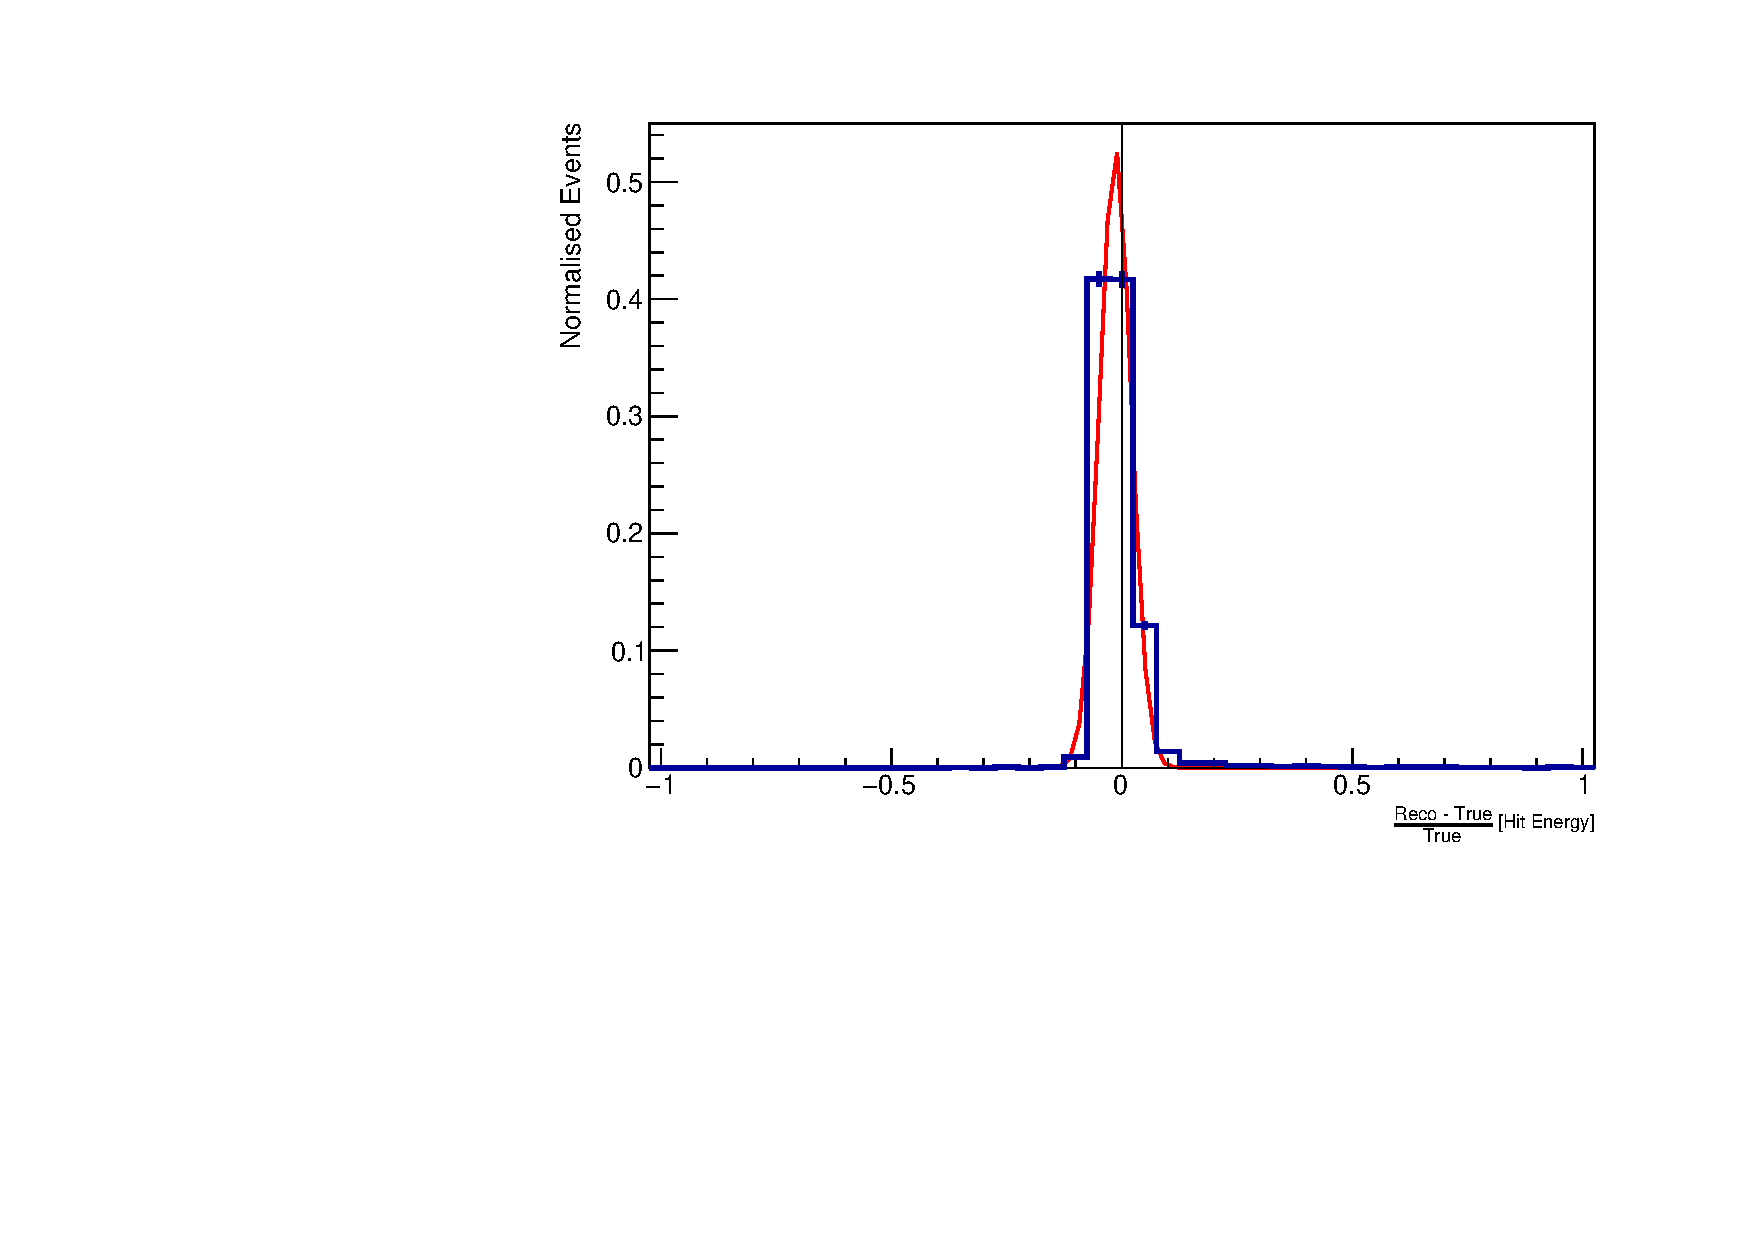
\includegraphics[width = 0.49\textwidth]{figures-chap4/hist_gauss_fit/linear_hit_only.pdf}
    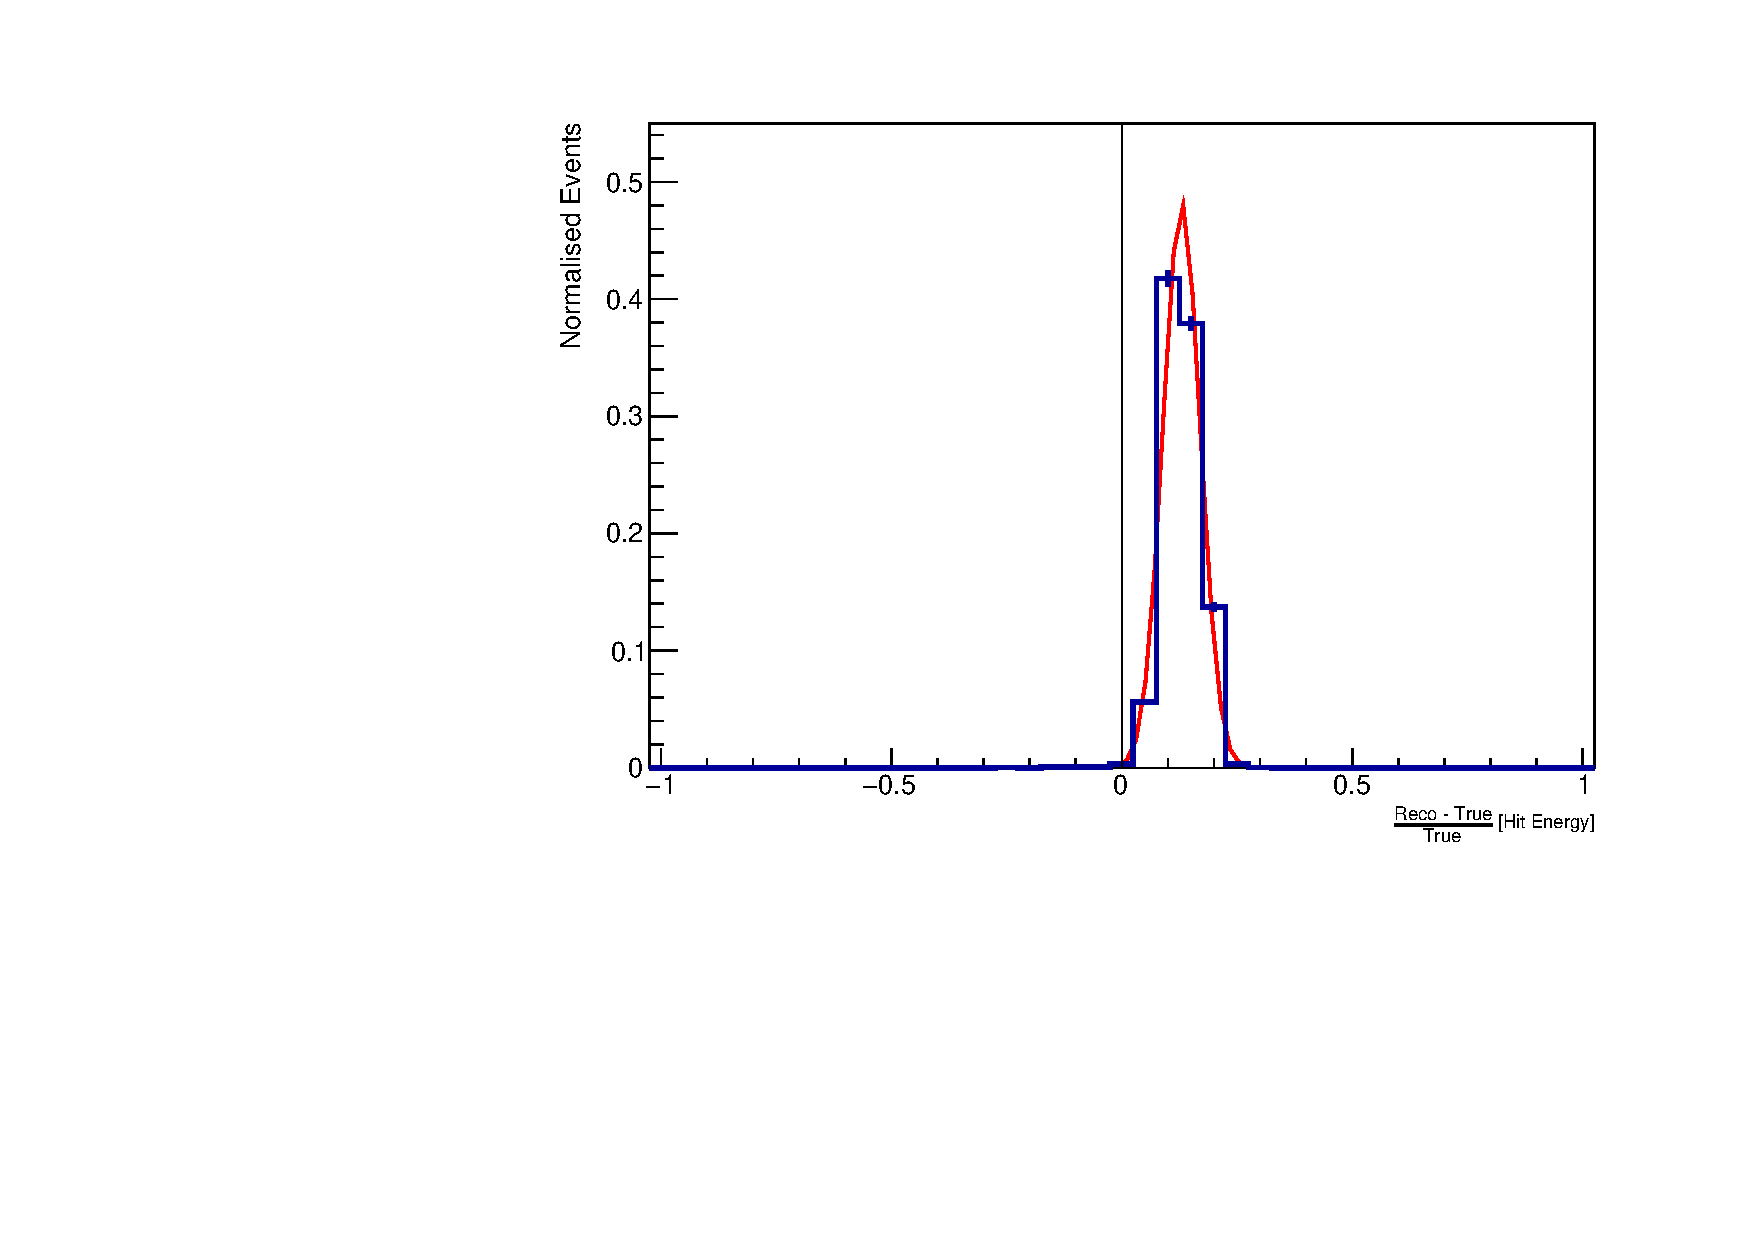
\includegraphics[width = 0.49\textwidth]{figures-chap4/hist_gauss_fit/oldmethod_hit_only.pdf}
    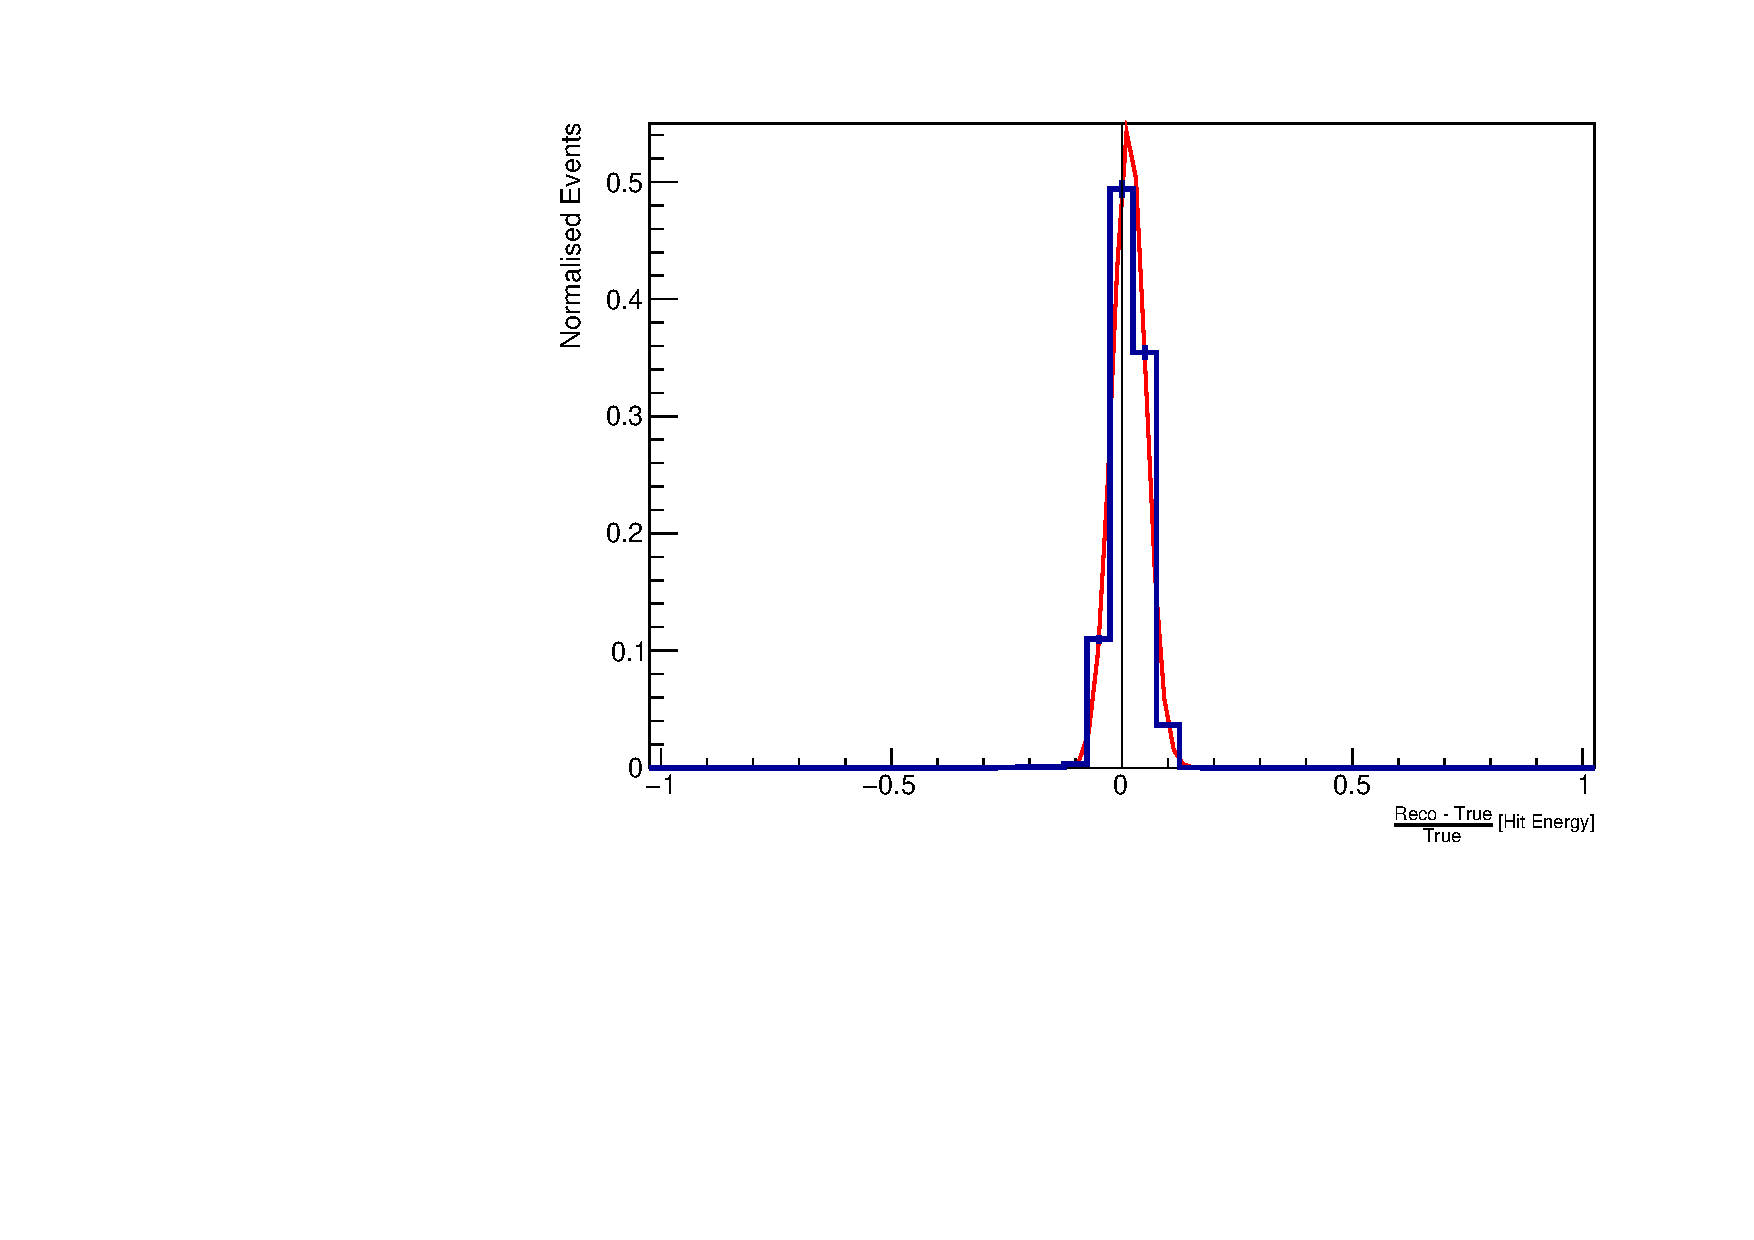
\includegraphics[width = 0.49\textwidth]{figures-chap4/hist_gauss_fit/ESTAR_hit_only.pdf}
    \captionsetup{width=0.45\textwidth}
    \parbox[b]{0.49\textwidth}%
  {
    \caption[Fractional energy separation using the true energy of the hits with a Gaussian fitted to the distribution.]
    {The fractional energy separation using the true energy of the hits with an associated Gaussian fit of the entire distribution. Top Left: \textit{Shower Linear Energy tool}, Top Right: \textit{Shower Num Electrons Energy tool} and Bottom Left: \textit{Shower ESTAR Energy tool}. \\}
    \label{fig:gauss_fit_hit_level}}
\end{figure}

\begin{figure}[h!]
    \centering
    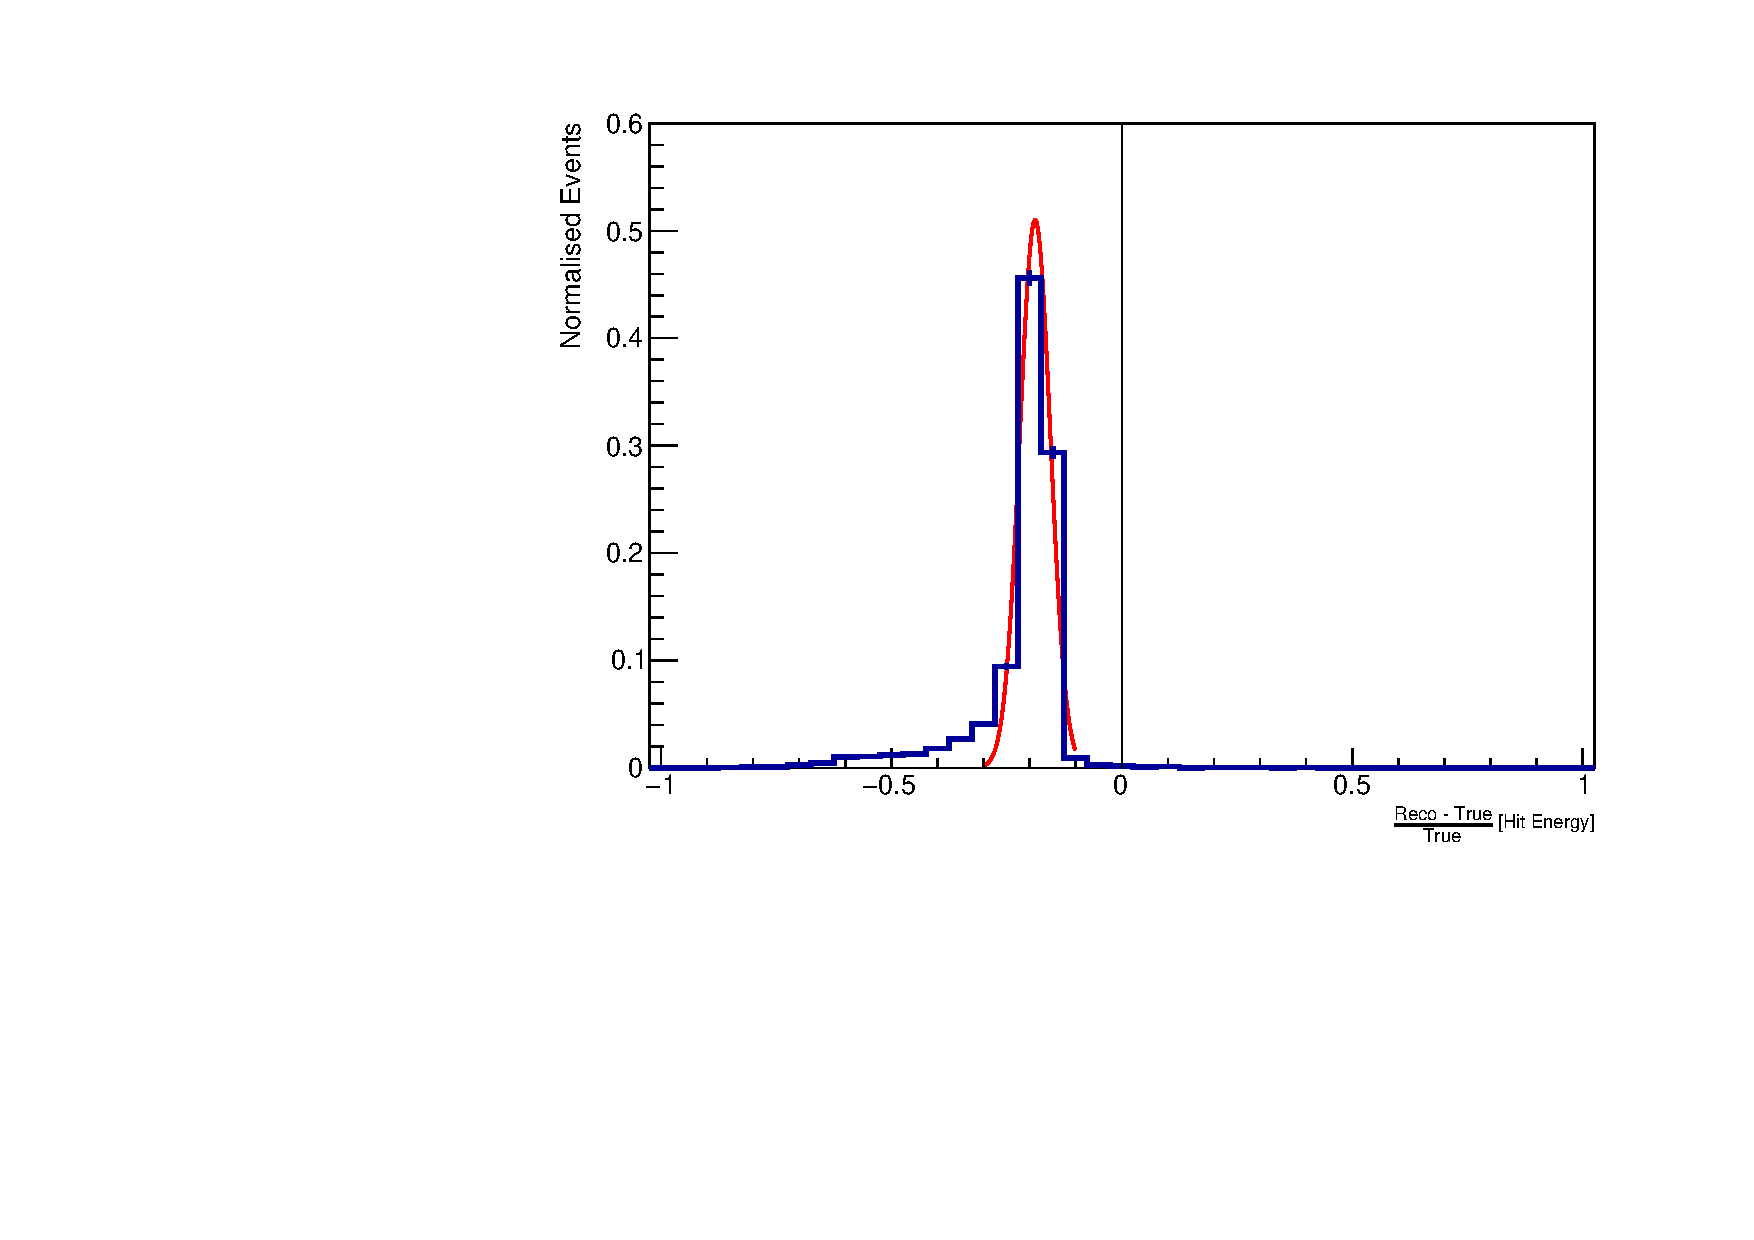
\includegraphics[width = 0.49\textwidth]{figures-chap4/hist_gauss_fit/linear_showering_e.pdf}
    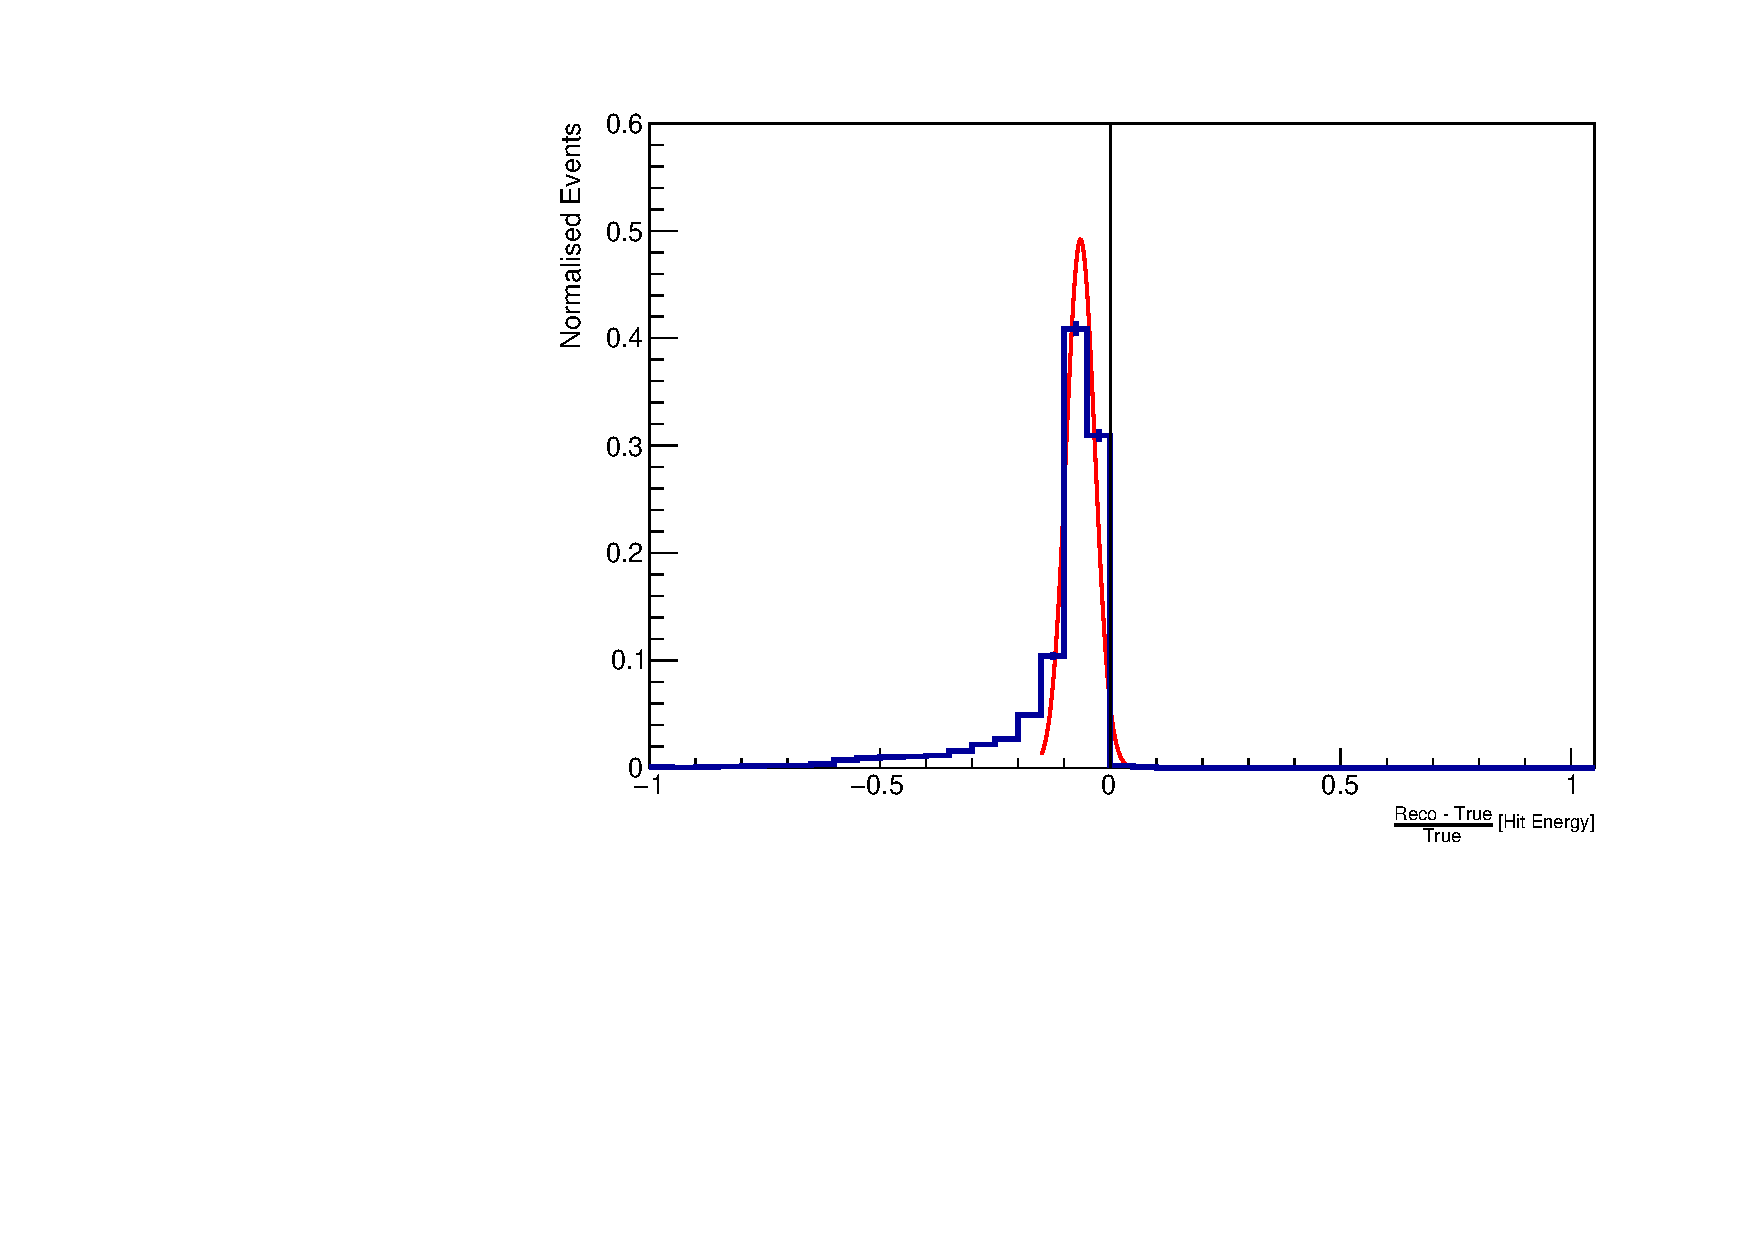
\includegraphics[width = 0.49\textwidth]{figures-chap4/hist_gauss_fit/oldmethod_showering_e_attempt2.pdf}
    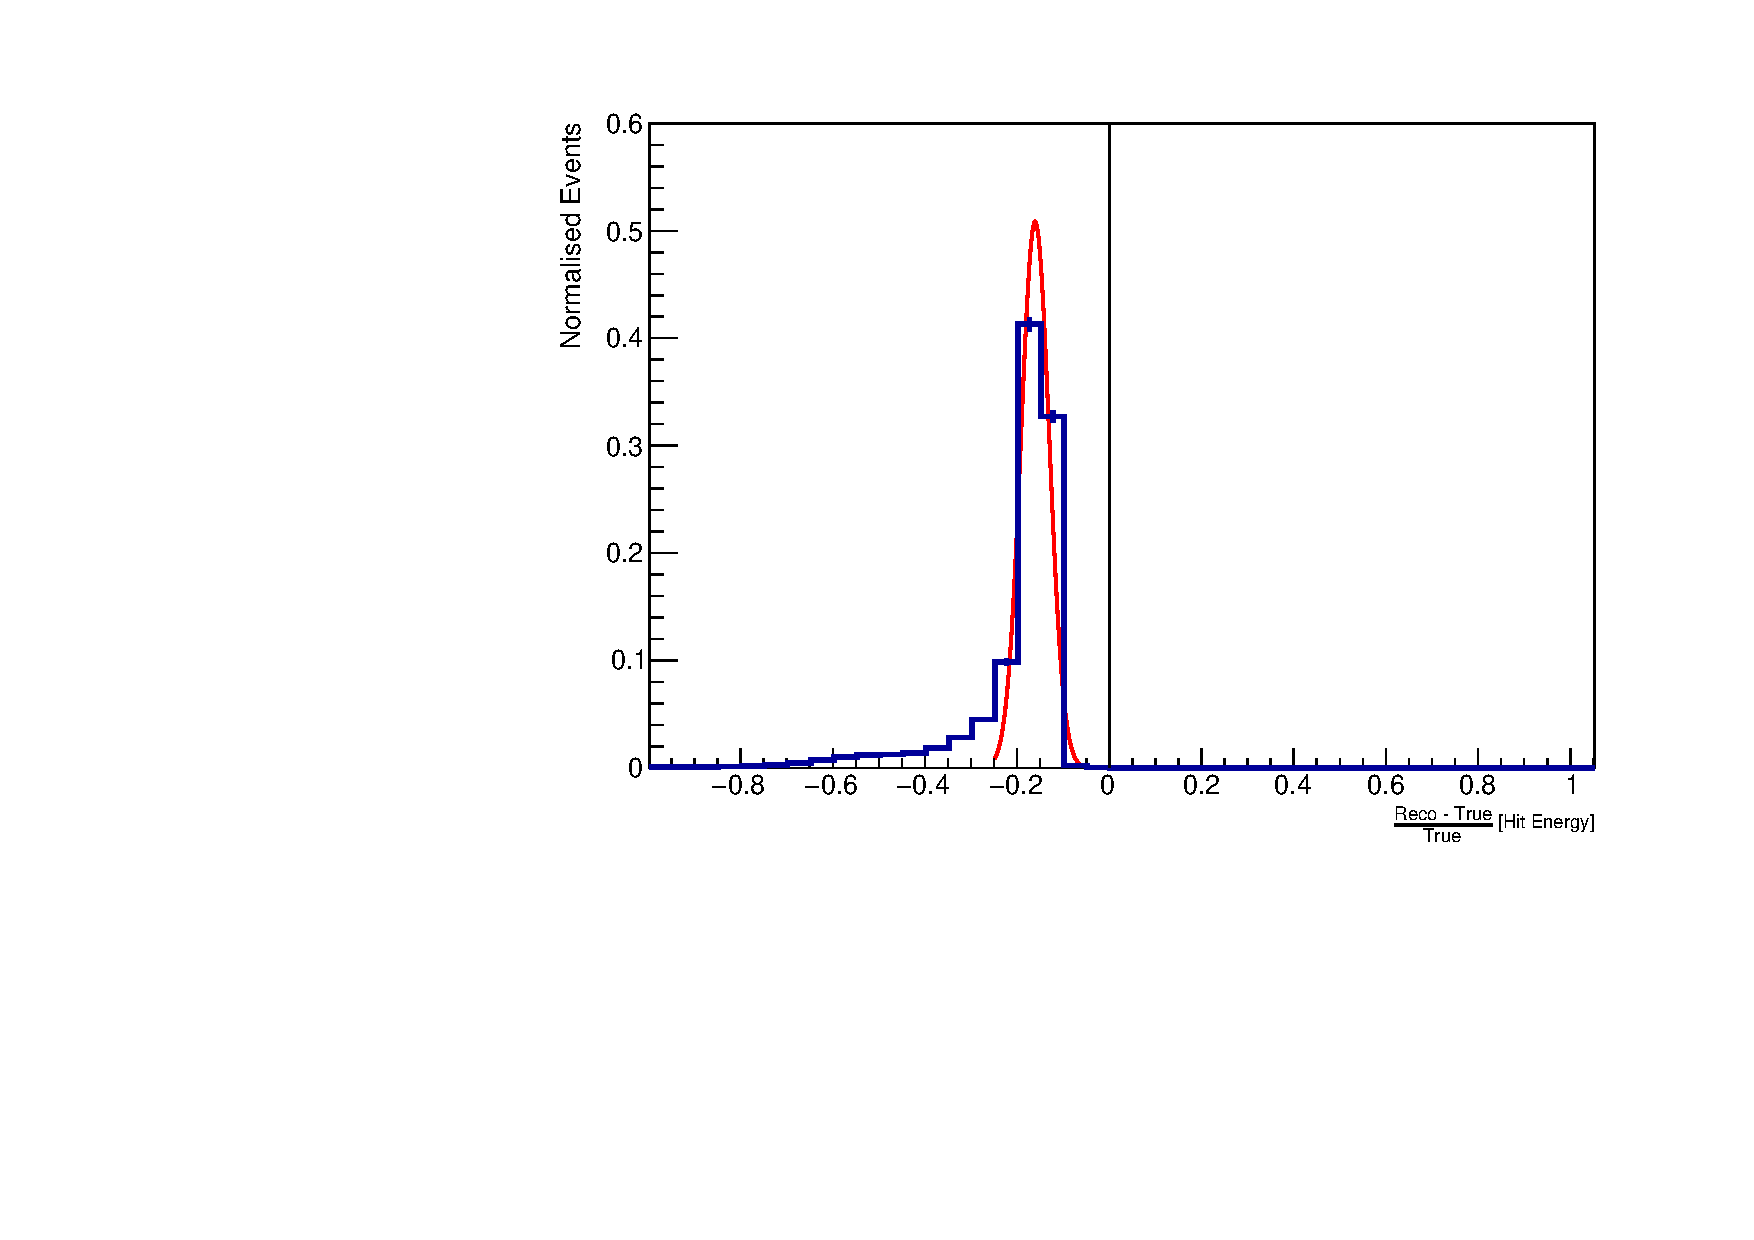
\includegraphics[width = 0.49\textwidth]{figures-chap4/hist_gauss_fit/ESTAR_showering_e_attempt2.pdf}
    \captionsetup{width=0.45\textwidth}
    \parbox[b]{0.49\textwidth}%
  {
    \caption[Fractional energy separation using the true energy of the showering electron with a Gaussian fitted to the distribution.]
    {The fractional energy separation using the true energy of the showering electron with an associated Gaussian fit of the entire distribution. Top Left: \textit{Shower Linear Energy tool}, Top Right: \textit{Shower Num Electrons Energy tool} and Bottom Left: \textit{Shower ESTAR Energy tool}. \\}
    \label{fig:gauss_fit_showering_e}}
\end{figure}

\newpage

\begin{table}[h!]
\begin{tabular}{lcc}
 & \multicolumn{2}{c}{$\sigma$ of the Gaussian Fit} \\
Algorithm & Hits & Showering Electron \\ \hline
Linear & 0.034  & 0.033 \\
Num of Electrons & 0.040 & 0.031 \\
ESTAR & 0.036 & 0.031
\end{tabular}
\caption[The $\sigma$ value used in the Gaussian fit to the fractional energy separation distributions of each algorithm.]{The $\sigma$ value used in the Gaussian fit to the fractional energy separation distributions of each algorithm. Both the distributions which use the true energy of the hits (\FigureRef{fig:gauss_fit_hit_level}) and the true energy of the showering electron (\FigureRef{fig:gauss_fit_showering_e}) are shown.}
\label{table:gaus_fit_sigma_values}
\end{table}

\newpage
To confirm that the reconstruction performance is comparable across all wire planes, the true vs reconstructed energy was also plotted for the two induction planes using the ESTAR method. This is shown in \FigureRef{fig:true_vs_reco_for_induction_planes} where the comparison has been made with the true energy of the hits.

\begin{figure}[h!]
    \centering
    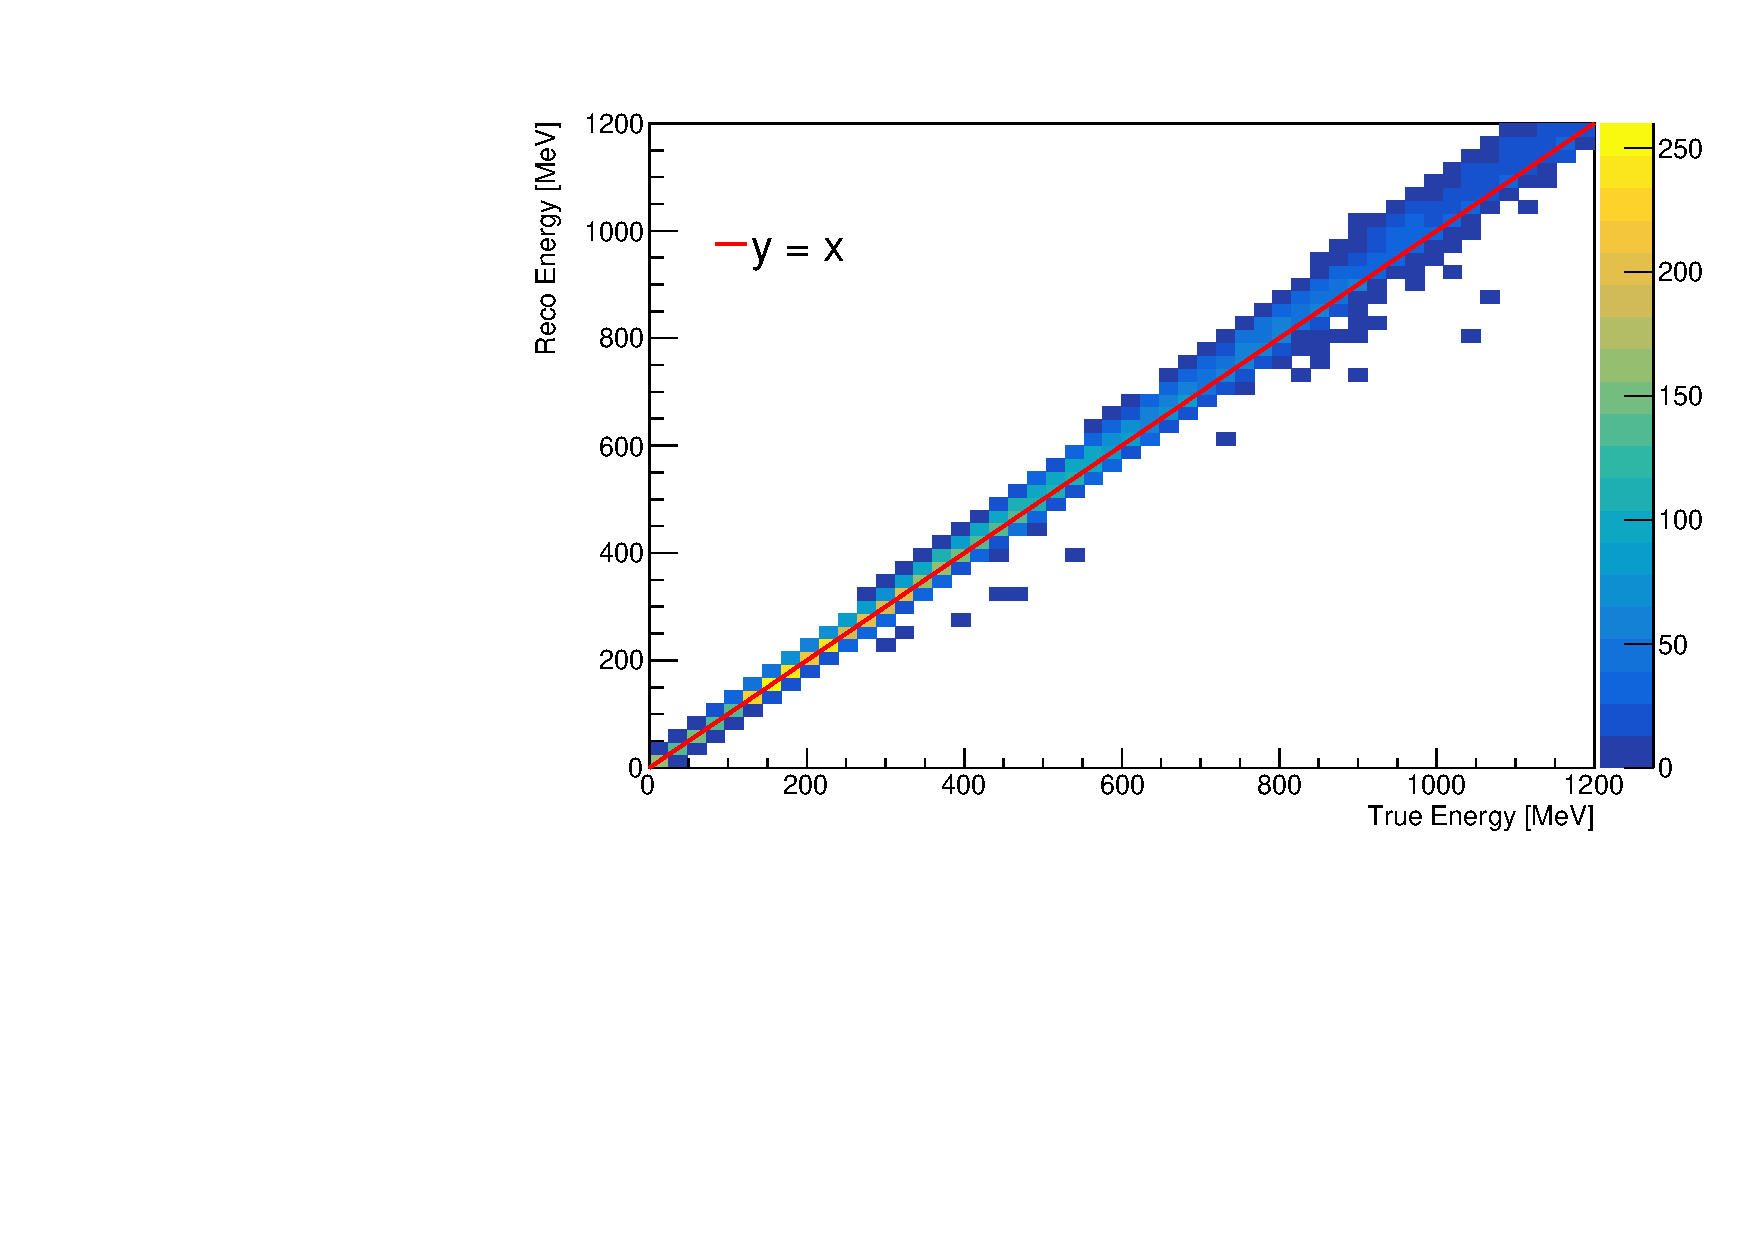
\includegraphics[width = 0.49\textwidth]{figures-chap4/true_vs_reco_plane0_ESTAR.pdf}
    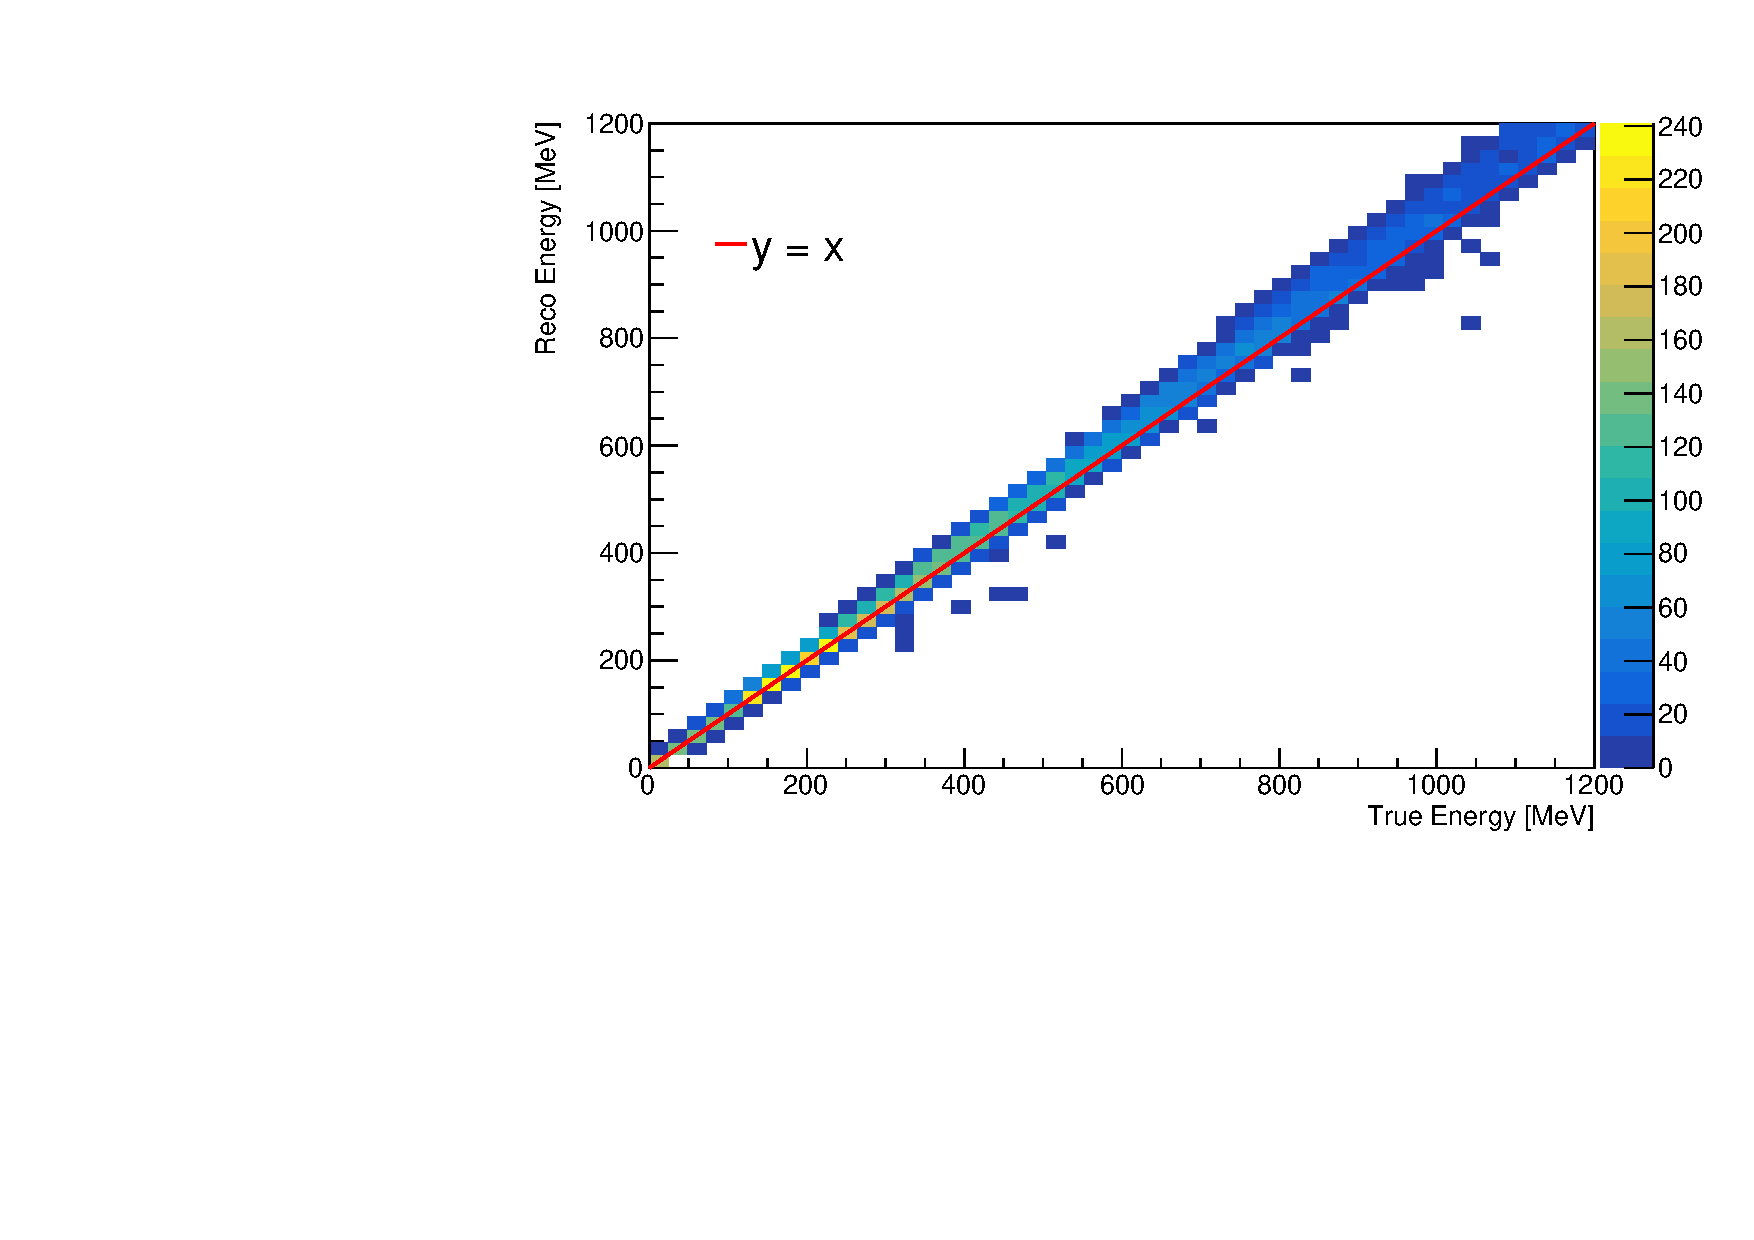
\includegraphics[width = 0.49\textwidth]{figures-chap4/true_vs_reco_plane1_ESTAR.pdf}
    \caption[True vs reconstructed energy from a showering electron for the two induction planes using the ESTAR method. The true energy has been evaluated from the hits of each shower.]{True vs reconstructed energy from a showering electron for the first induction plane (Left) and the second induction plane (Right) using the ESTAR method. The true energy has been evaluated from the hits of each shower.}
    \label{fig:true_vs_reco_for_induction_planes}
\end{figure}

Since photons also produce \gls{em} showers, a \gls{bnb}-like $\gamma + \pi^+$ sample was produced to verify that the reconstruction works equally well in this case. \FigureRef{fig:true_vs_reco_photon_sample} shows this using the ESTAR method with the hits from the collection plane. 

\begin{figure}
    \centering
    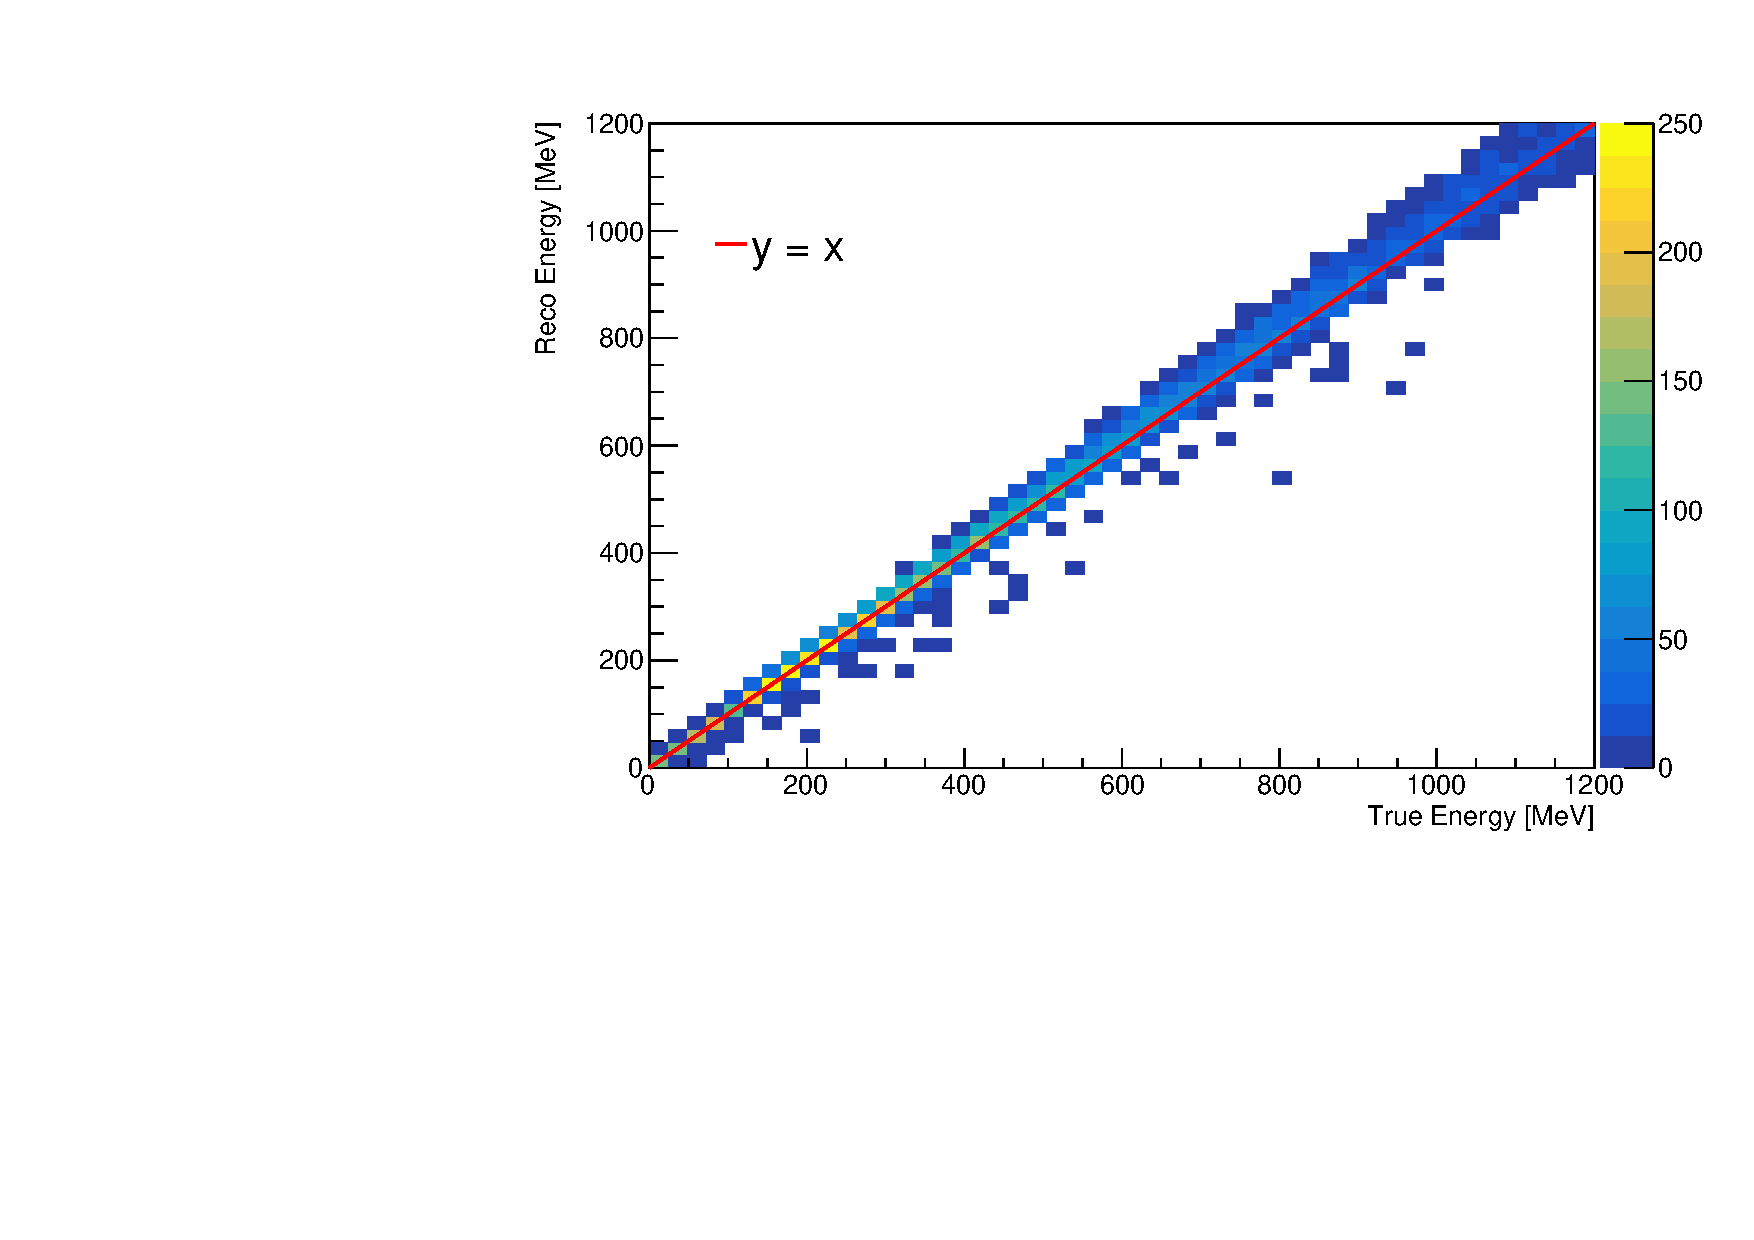
\includegraphics[width = \largefigwidth]{figures-chap4/true_vs_reco_photon_ESTAR.pdf}
    \caption[True vs reconstructed energy from a showering photon using the ESTAR method. The true energy has been evaluated from the hits of each shower.]{True vs reconstructed energy from a showering photon using the ESTAR method with the hits from the collection plane. The true energy has been evaluated from the hits of each shower.}
    \label{fig:true_vs_reco_photon_sample}
\end{figure}

\clearpage
\subsection{Performance as a Function of Angle}

From a \gls{bnb} neutrino sample, most of the showers are expected to be predominantly forward-going. A fraction of showers will however be directed at large angles to the beamline. As was mentioned in \SectionRef{sec:Event Production and Reconstruction}, showers directed towards the wire planes tend to produce waveforms which are not well represented by Gaussians. Since the \textit{GausHitFinder} has trouble applying a suitable fit to these cases, a degradation in the reconstruction performance is expected as a function of angle.

In order to verify this, an  $e^- + \pi^+$ sample was produced with the electron being directed in all $\theta_{xz}$ angles. Otherwise, this sample is also \gls{bnb}-like. $\theta_{xz}$ is the angle between the beamline and the positive x-direction and is defined in terms of the \gls{sbnd} coordinate system which is shown in \FigureRef{fig:sbnd_coordinate_system}. The reconstruction performance is shown in \FigureRef{fig:reconstruction_as_a_function_of_angle} using the ESTAR method for both definitions of true energy. Profiles of the histograms in \FigureRef{fig:reconstruction_as_a_function_of_angle} are shown in \FigureRef{fig:reconstruction_as_a_function_of_angle_profile} where the y-axis error bars are the standard deviations. As is expected, a degradation in the reconstruction performance is observed in both cases as $\theta_{xz}$ tends away from $0^\circ$. It should be noted that the degradations are in opposite directions which may be explained by the fact that at large angles, the reconstruction method tends to overestimate the energy of the available hits, but the hit reconstruction also suffers, so the overall fraction of hits representing the shower is reduced. Both the \textit{Shower Linear Energy tool} and \textit{Shower Num Electrons Energy tool} have a constant recombination correction and therefore the conversion from charge to energy is linear. The \textit{Shower ESTAR Energy tool} is not perfectly linear but it is close, especially in the region up to $\mathcal{O}(10 \text{ MeV})$. Therefore, there is essentially no angular variation among the three methods so results akin to \FigureRef{fig:reconstruction_as_a_function_of_angle} for the \textit{Shower Linear Energy tool} and the \textit{Shower Num of Electrons Energy tool} would look almost identical only with the y-axis scaled appropriately. 
\begin{figure}[h!]
    \centering
    
    \begin{tikzpicture}[x=1cm, y=1cm, z=-0.6cm]
        \draw (0,0) node (O) {};
        % Axes
        \draw [->] (0,0,0) -- (-4,0,0) node (x) [left, at end] {$x$}; %[above] {$x$};
        \draw [->] (0,0,0) -- (0,4,0) node (y) [above] {$y$};
        \draw [->] (0,0,0) -- (0,0,-4) node [right, xshift=-0.25em, yshift=0.5em] (z) {$z$};
    
        \pic [draw=red, ->, "\textcolor{red}{$\theta_{xz}$}", angle radius=1.3cm, angle  eccentricity=1.3] {angle = z--O--x};
        \pic [draw=teal, ->, "\textcolor{teal}{$\theta_{yz}$}", angle radius=0.7cm, angle eccentricity=1.45] {angle = z--O--y};

    \end{tikzpicture}

    \caption[The \gls{sbnd} coordinate system.]{The \gls{sbnd} coordinate system. The origin is located at the centre of the upstream face of the detector which is defined to be at (0, 200, 0) cm with the \textit{z} direction being along the beamline.}
    \label{fig:sbnd_coordinate_system}
\end{figure}


\begin{figure}[h!]
    \centering
    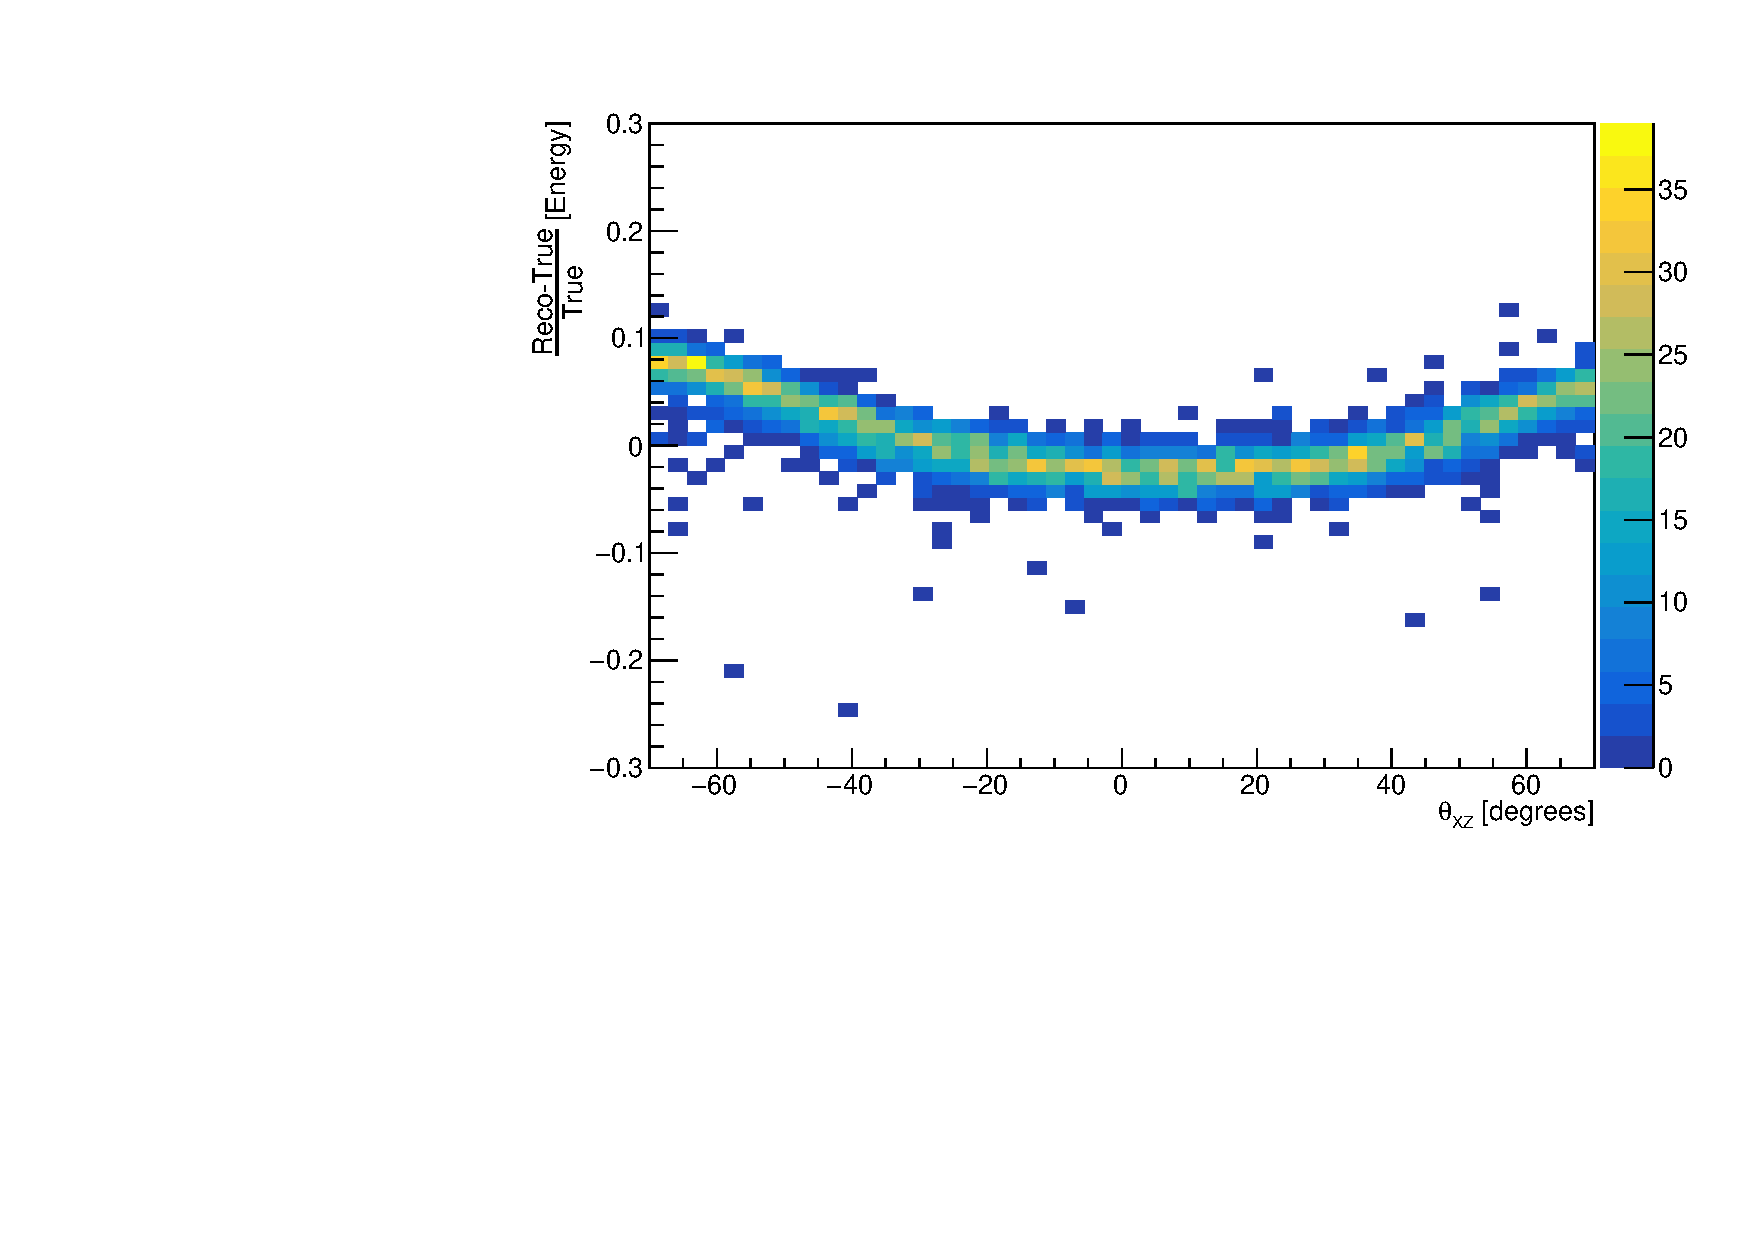
\includegraphics[width = 0.49\textwidth]{figures-chap4/frac_res_vs_thetaXZ_cheating_electron_vertex_plane2_cut.pdf}
    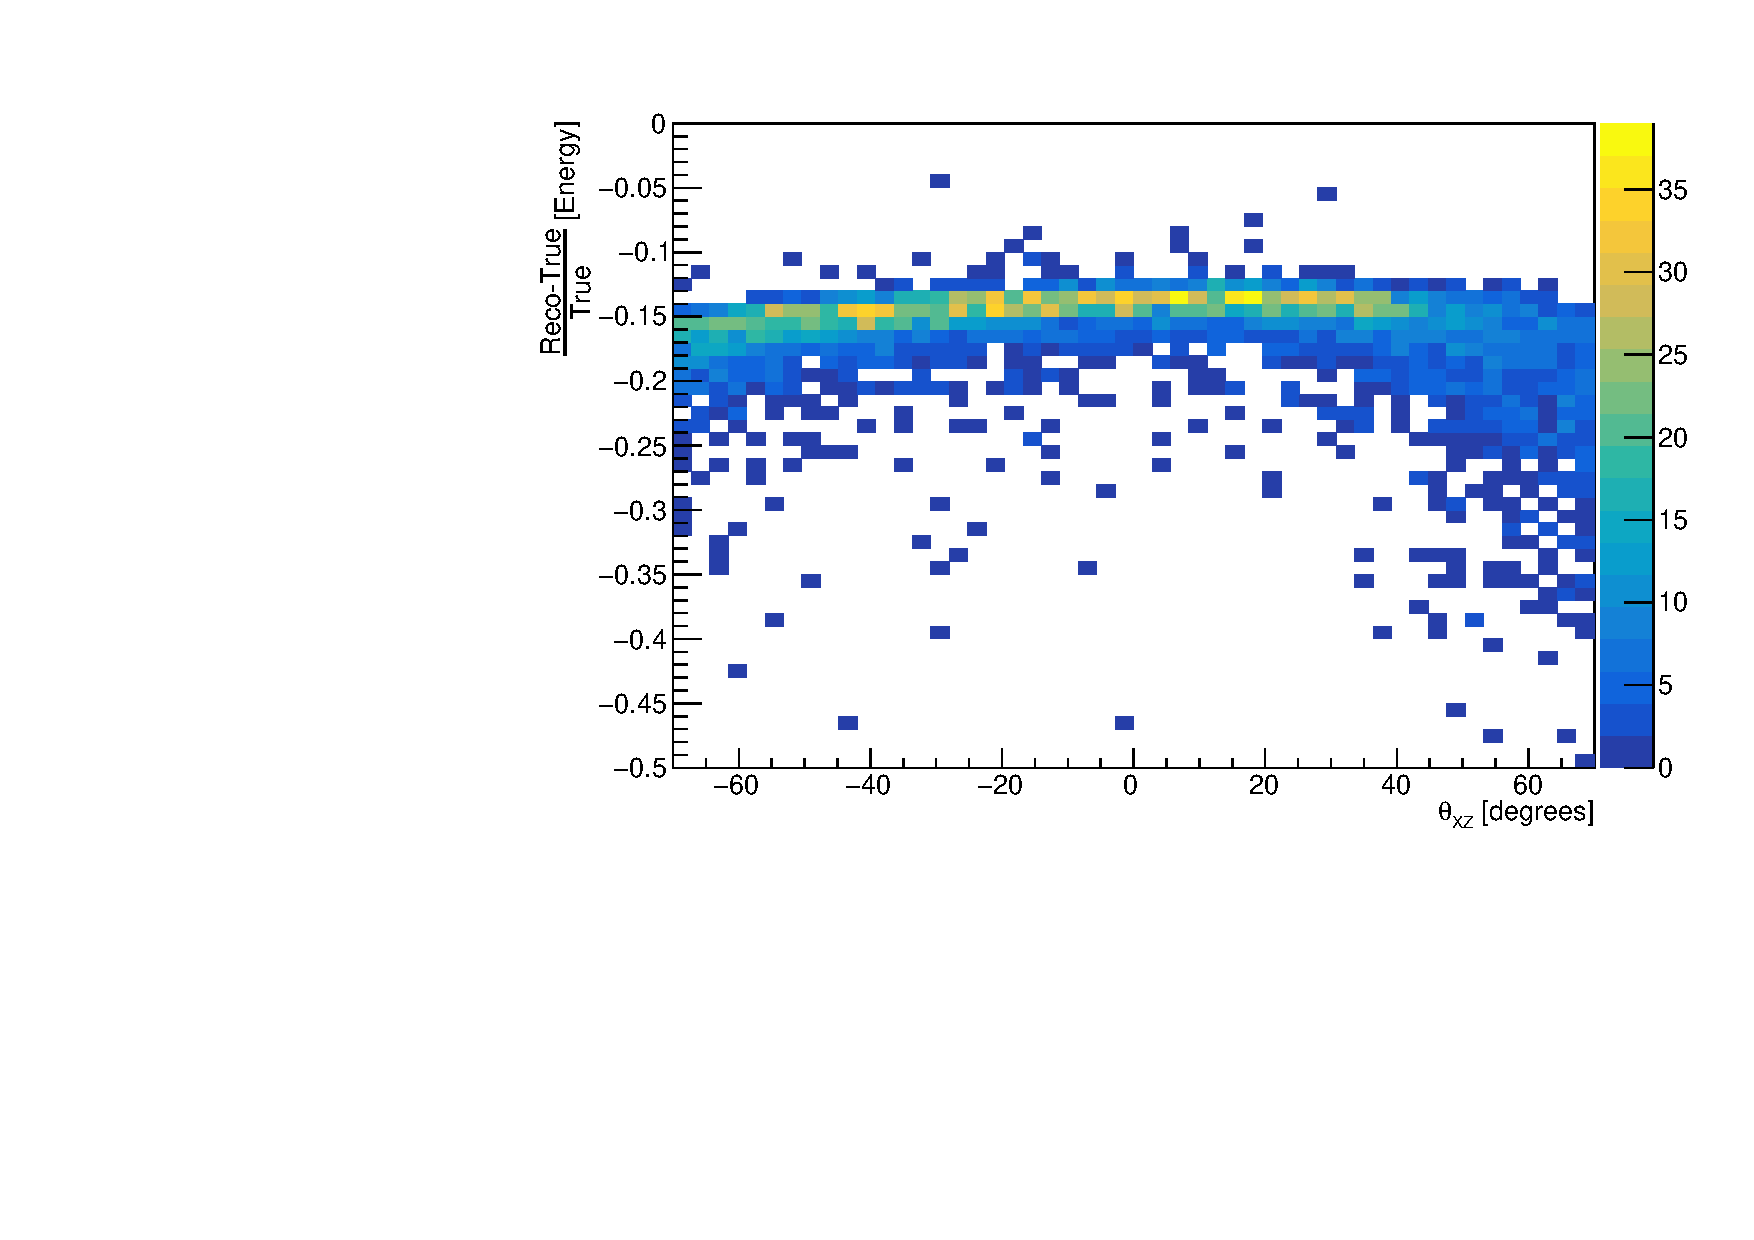
\includegraphics[width = 0.49\textwidth]{figures-chap4/frac_res_vs_thetaXZ_showeringE_cheating_electron_vertex_plane2_cut.pdf}
    \caption[The fractional energy separation as a function of $\theta_{xz}$.]{The fractional energy separations as a function of $\theta_{xz}$ using the ESTAR method. Left: true energy is calculated from the hits. Right: true energy is the energy of the showering electron.}
    \label{fig:reconstruction_as_a_function_of_angle}
\end{figure}

\begin{figure}[h!]
    \centering
    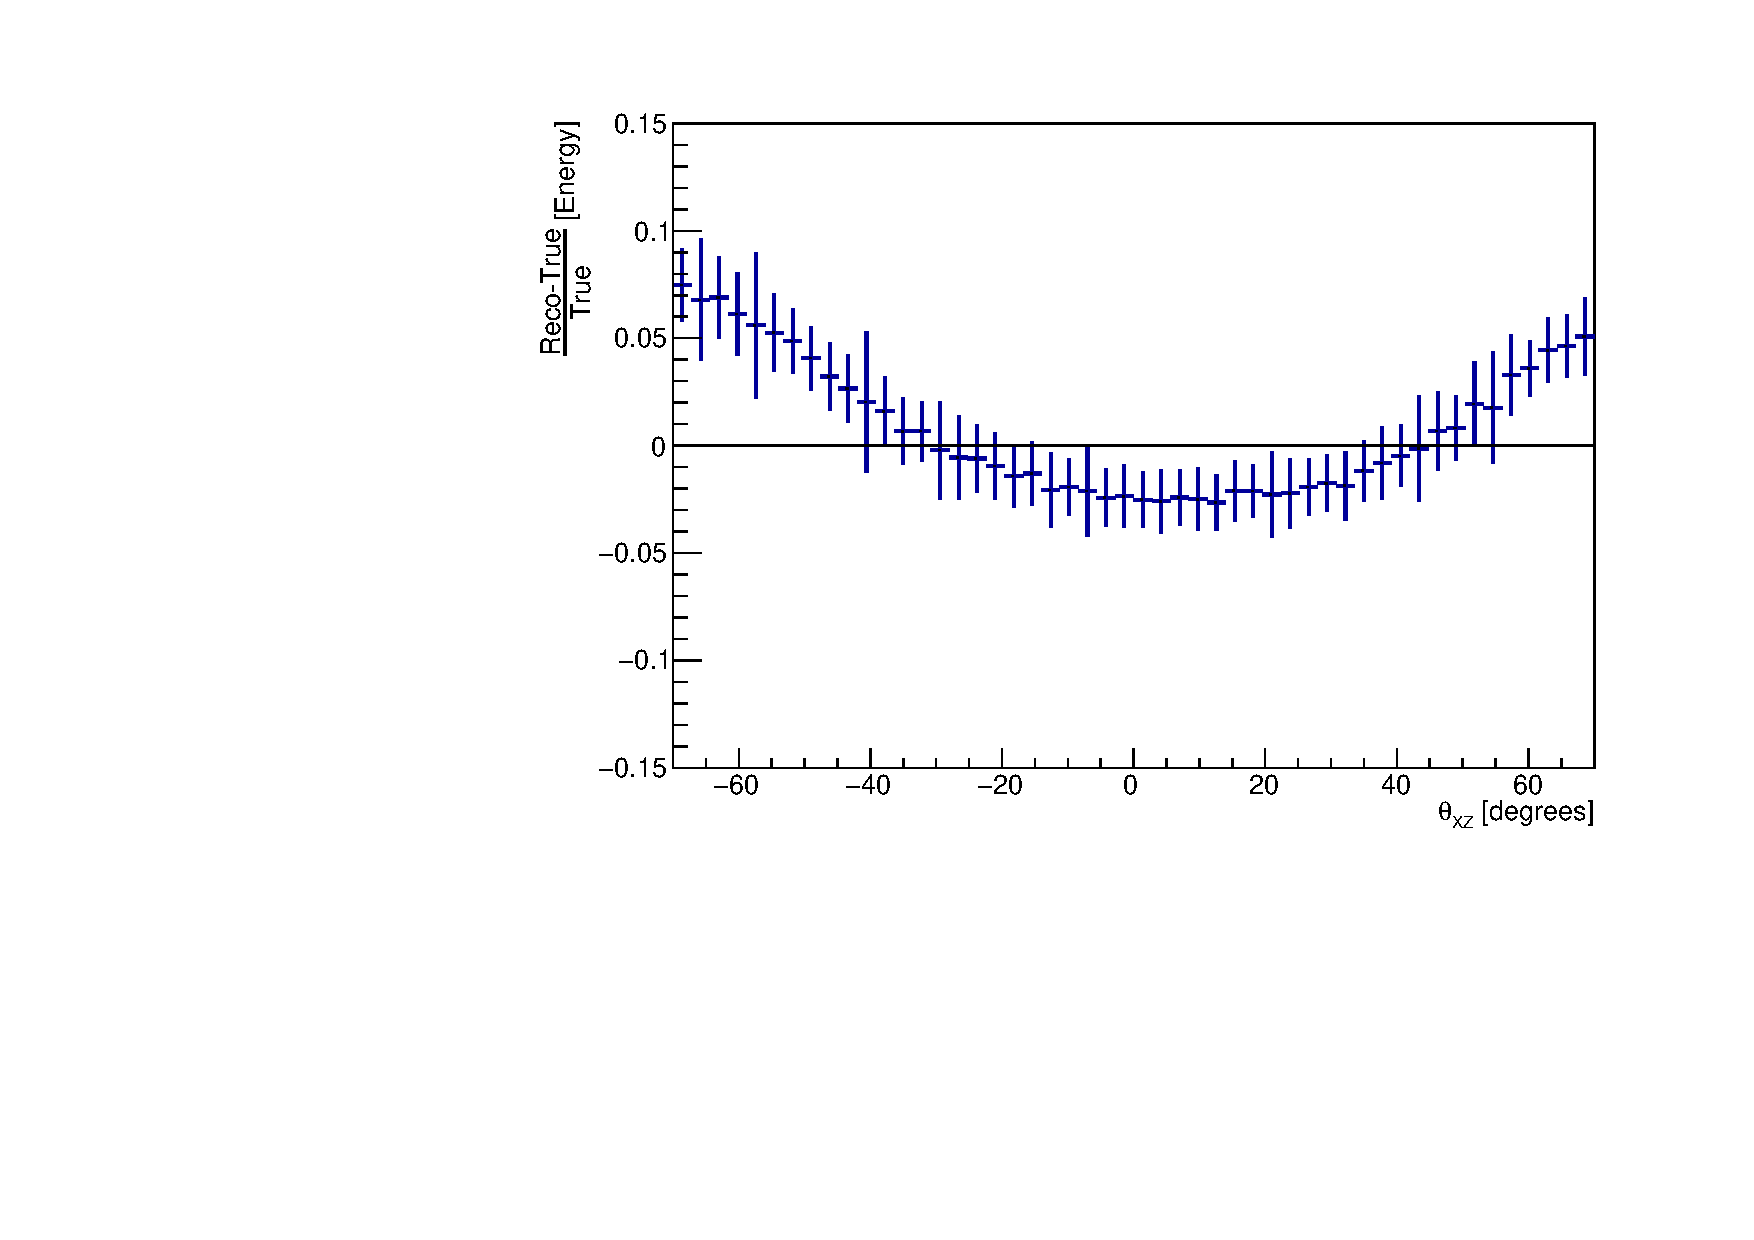
\includegraphics[width = 0.49\textwidth]{figures-chap4/frac_res_vs_thetaXZ_cheating_electron_vertex_plane2_cut_ESTAR_profile.pdf}
    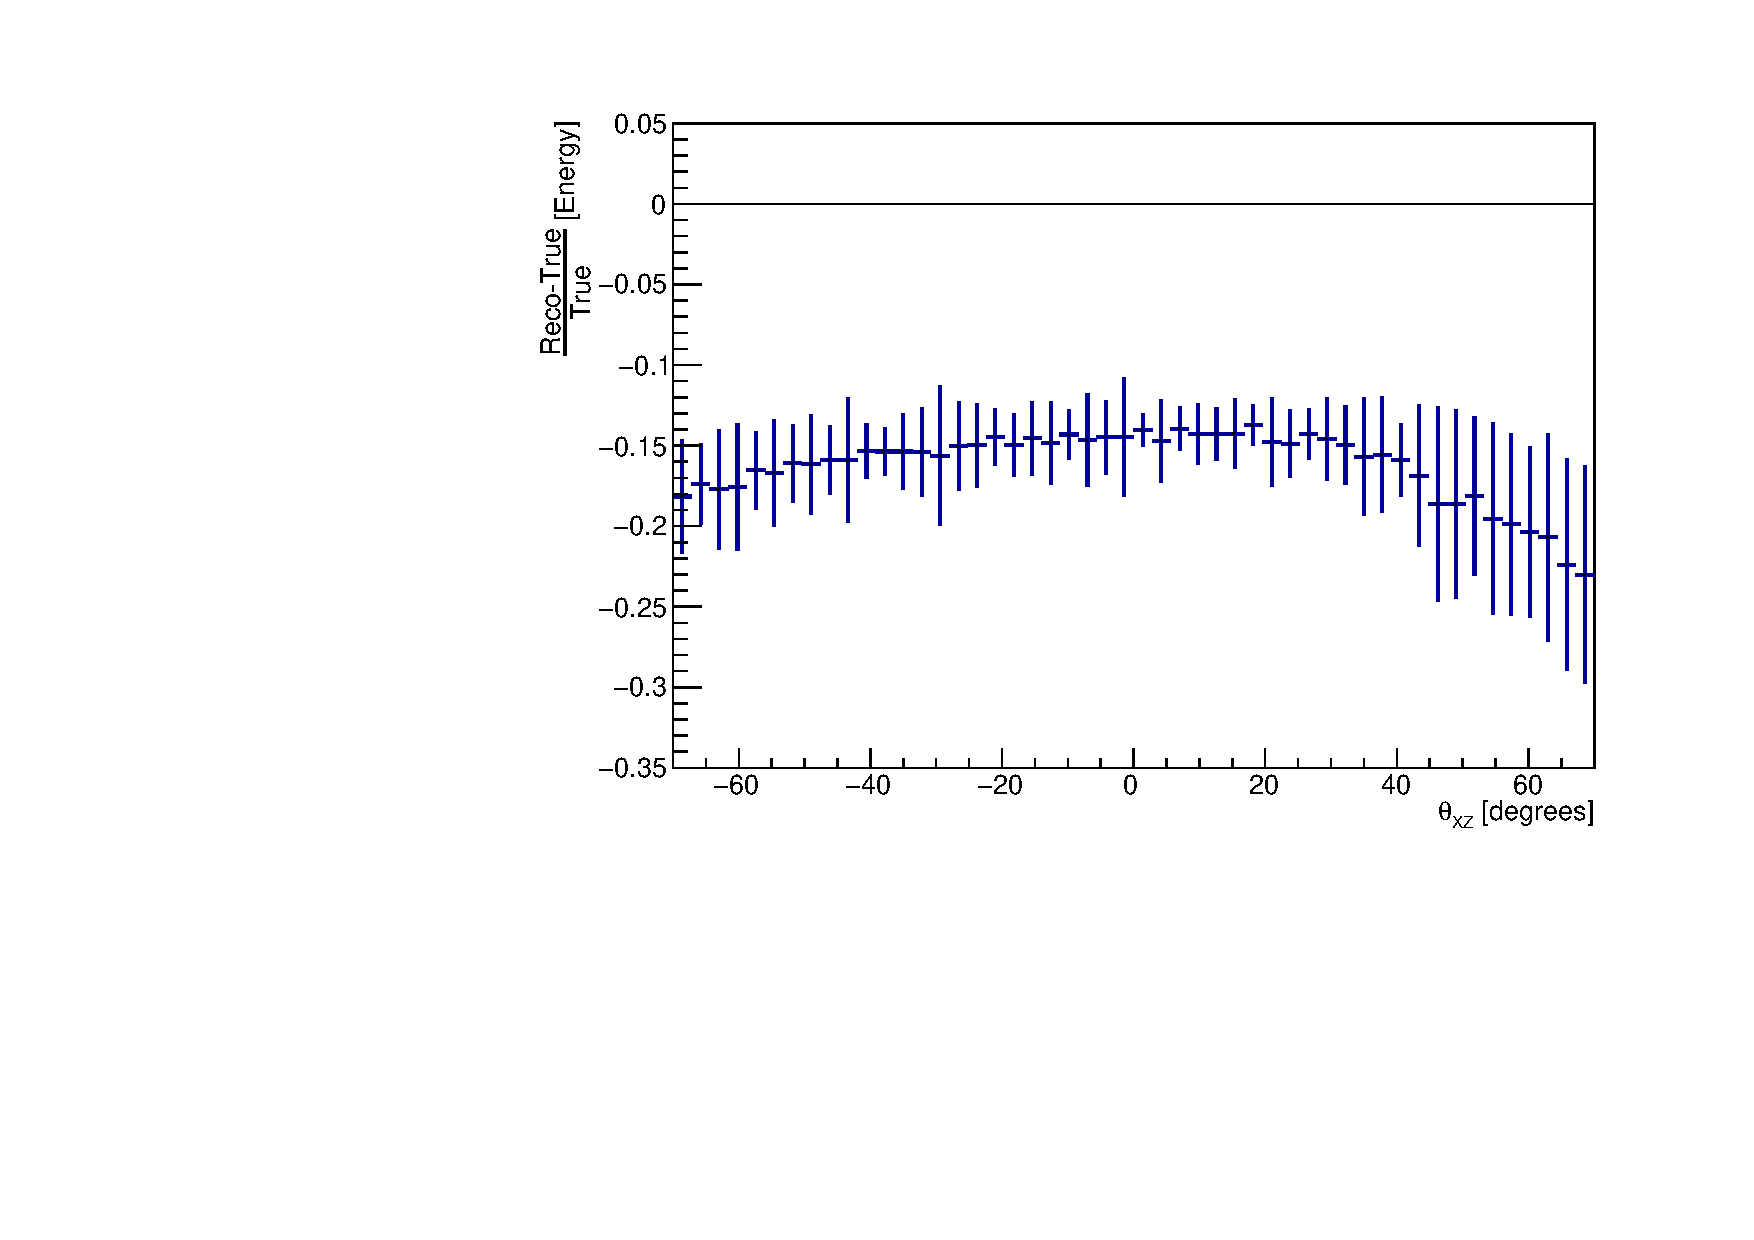
\includegraphics[width = 0.49\textwidth]{figures-chap4/frac_res_vs_thetaXZ_cheating_electron_vertex_plane2_cut_showeringE_ESTAR_profile.pdf}
    \caption[Profile histograms of the fractional energy separation as a function of $\theta_{xz}$.]{Profile histograms of the fractional energy separation as a function of $\theta_{xz}$ using the ESTAR method. The profile histograms are constructed from \FigureRef{fig:reconstruction_as_a_function_of_angle} and the y-axis error bars are the standard deviations.  Left: true energy is calculated from the hits. Right: true energy is the energy of the showering electron.}
    \label{fig:reconstruction_as_a_function_of_angle_profile}
\end{figure}

\clearpage
\subsection{Performance as a Function of Energy}
The \gls{em} showers produced in \gls{sbnd} from the \gls{bnb} are expected to have energies up to around a GeV. Since the energy range is relatively broad, the reconstruction performance is evaluated as a function of the energy in order to confirm that the reconstruction methods work sufficiently well for all energies. As was the case for the angular dependence, the performance as a function of true energy is expected to not be method dependent. The only difference would be a y-axis scaling due to the different reconstruction performances. 

On the whole, the fractional separation is observed to be fairly constant across all energies when comparing with both the true energy of the hits and the true energy of the showering particle as can be seen in \FigureRef{fig:reconstruction_as_a_function_of_energy}. The fractional energy separation is slightly lower at the lowest energies, especially when compared with the true energy of the showering particle. This is highlighted in \FigureRef{fig:reconstruction_as_a_function_of_energy_profile} which shows the profiles of the histograms of the fractional energy separation as a function of true energy and can likely be explained by a greater fraction of the hits not passing the threshold cut. 

\begin{figure}[h!]
    \centering
    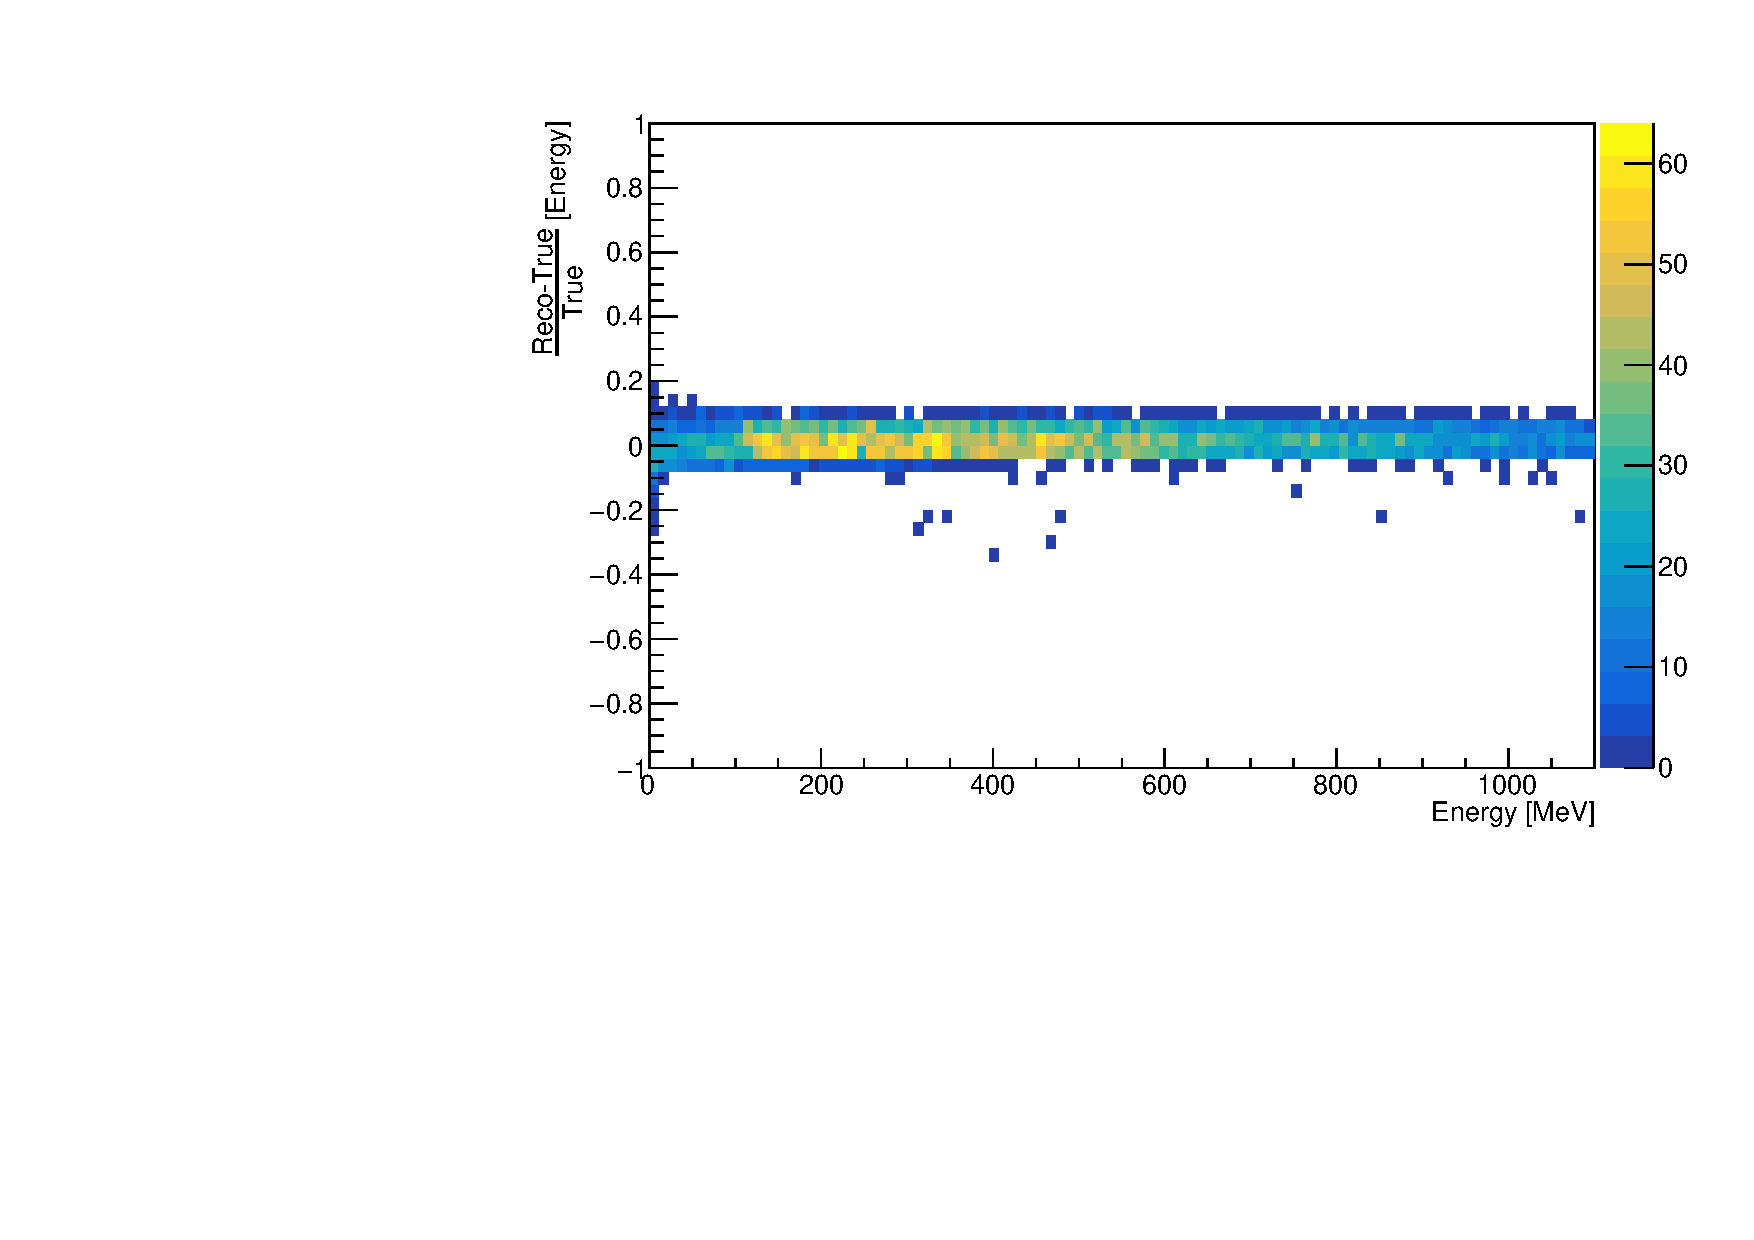
\includegraphics[width = 0.49\textwidth]{figures-chap4/frac_res_vs_energy_cheating_electron_vertex_plane2_ESTAR.pdf}
    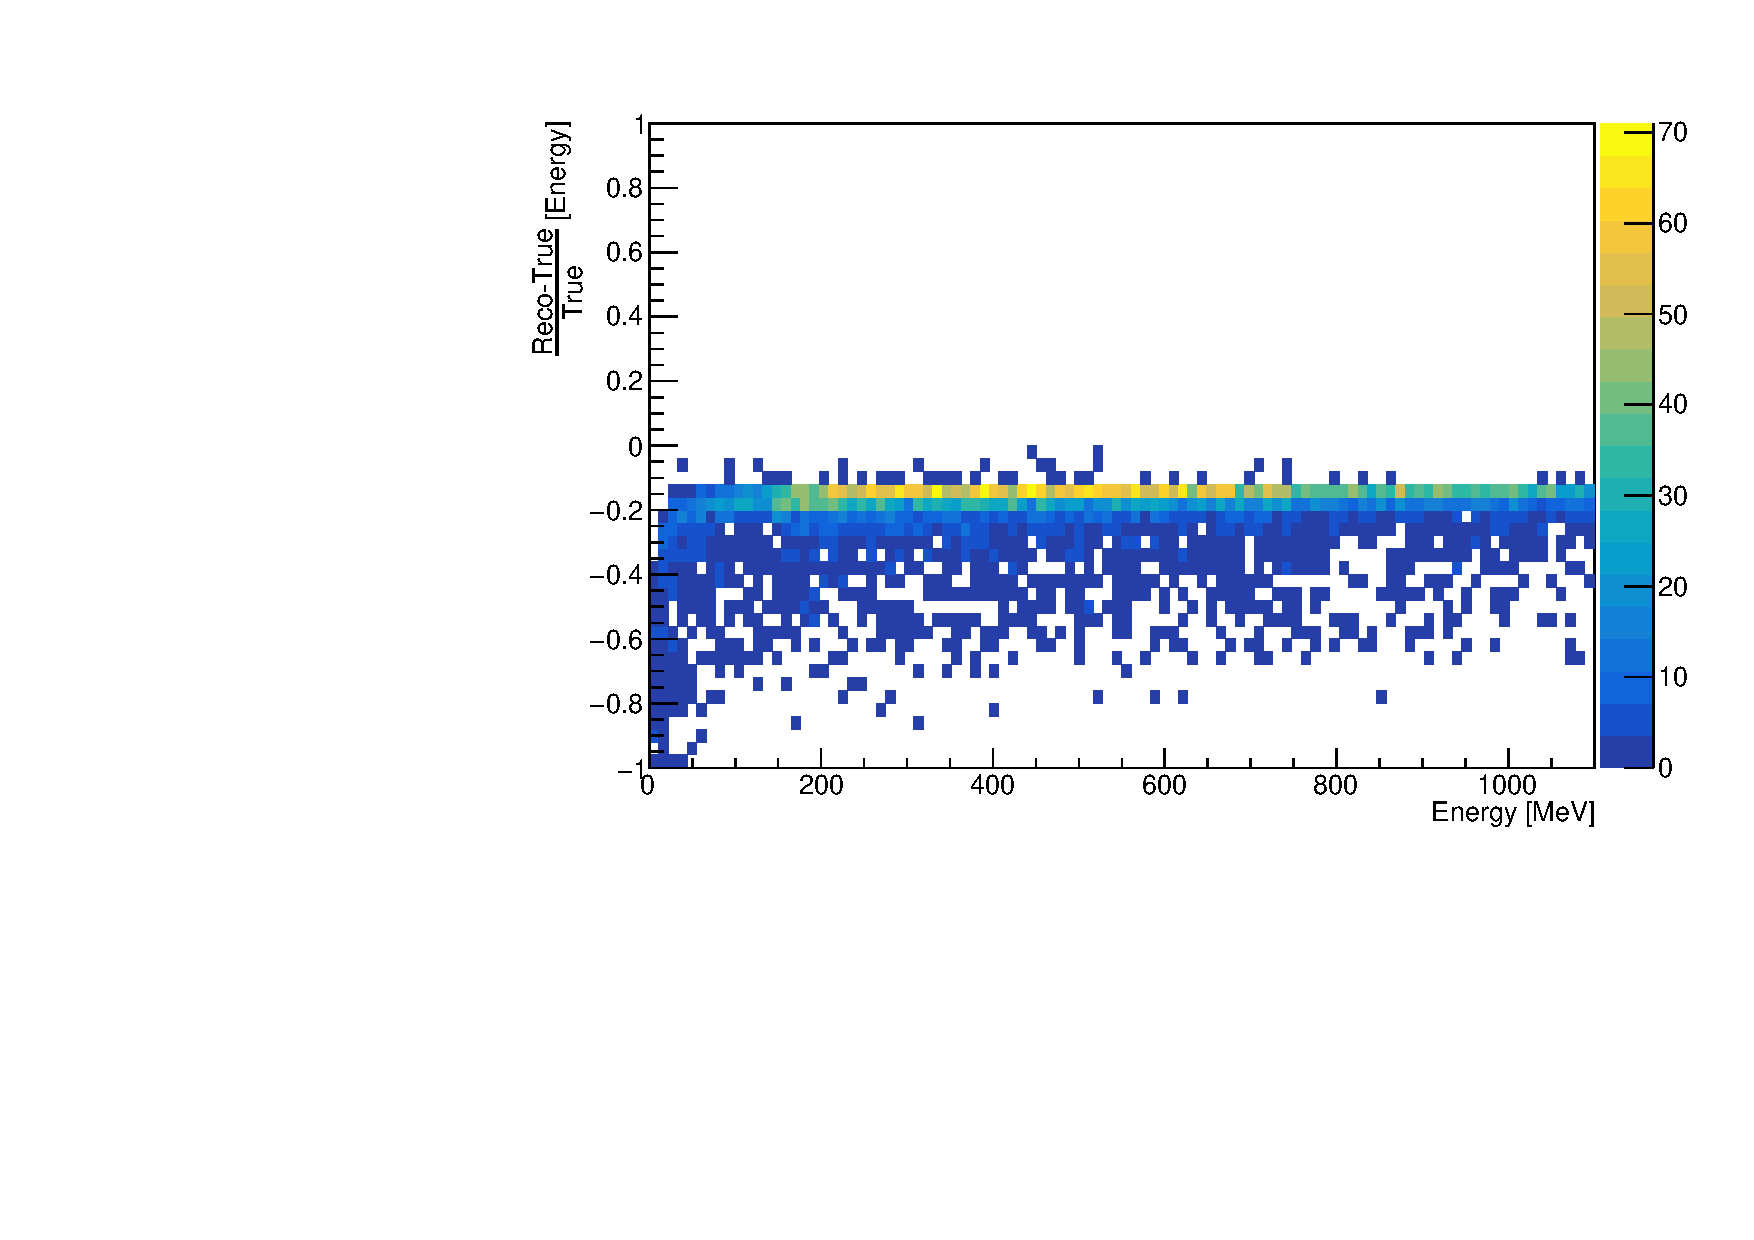
\includegraphics[width = 0.49\textwidth]{figures-chap4/frac_res_vs_energy_cheating_electron_vertex_plane2_ESTAR_showeringE.pdf}
    \caption[The fractional energy separations as a function of true energy.]{The fractional energy separations as a function of true energy using the ESTAR method. Left: true energy is calculated from the hits. Right: true energy is the energy of the showering electron.}
    \label{fig:reconstruction_as_a_function_of_energy}
\end{figure}


\begin{figure}[h!]
    \centering
    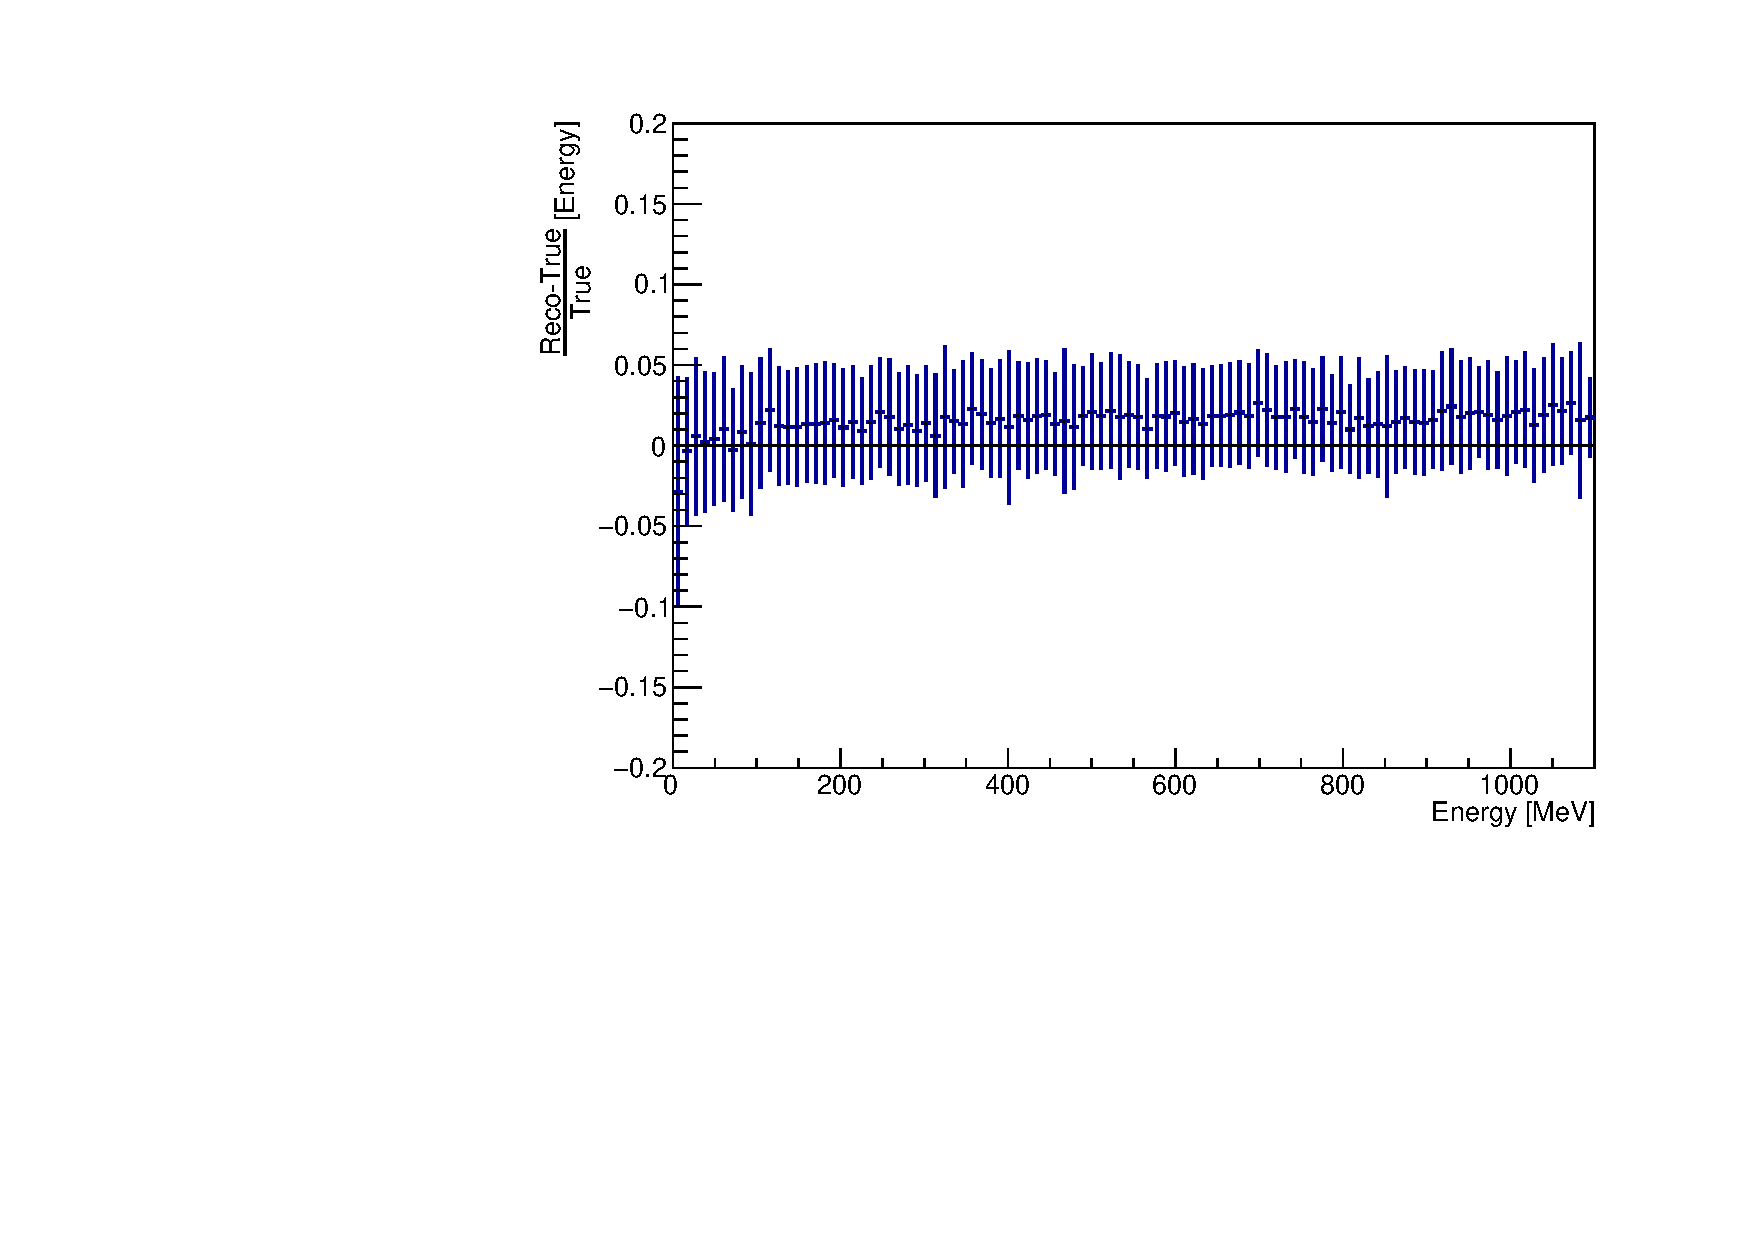
\includegraphics[width = 0.49\textwidth]{figures-chap4/frac_res_vs_energy_cheating_electron_vertex_plane2_ESTAR_profile.pdf}
    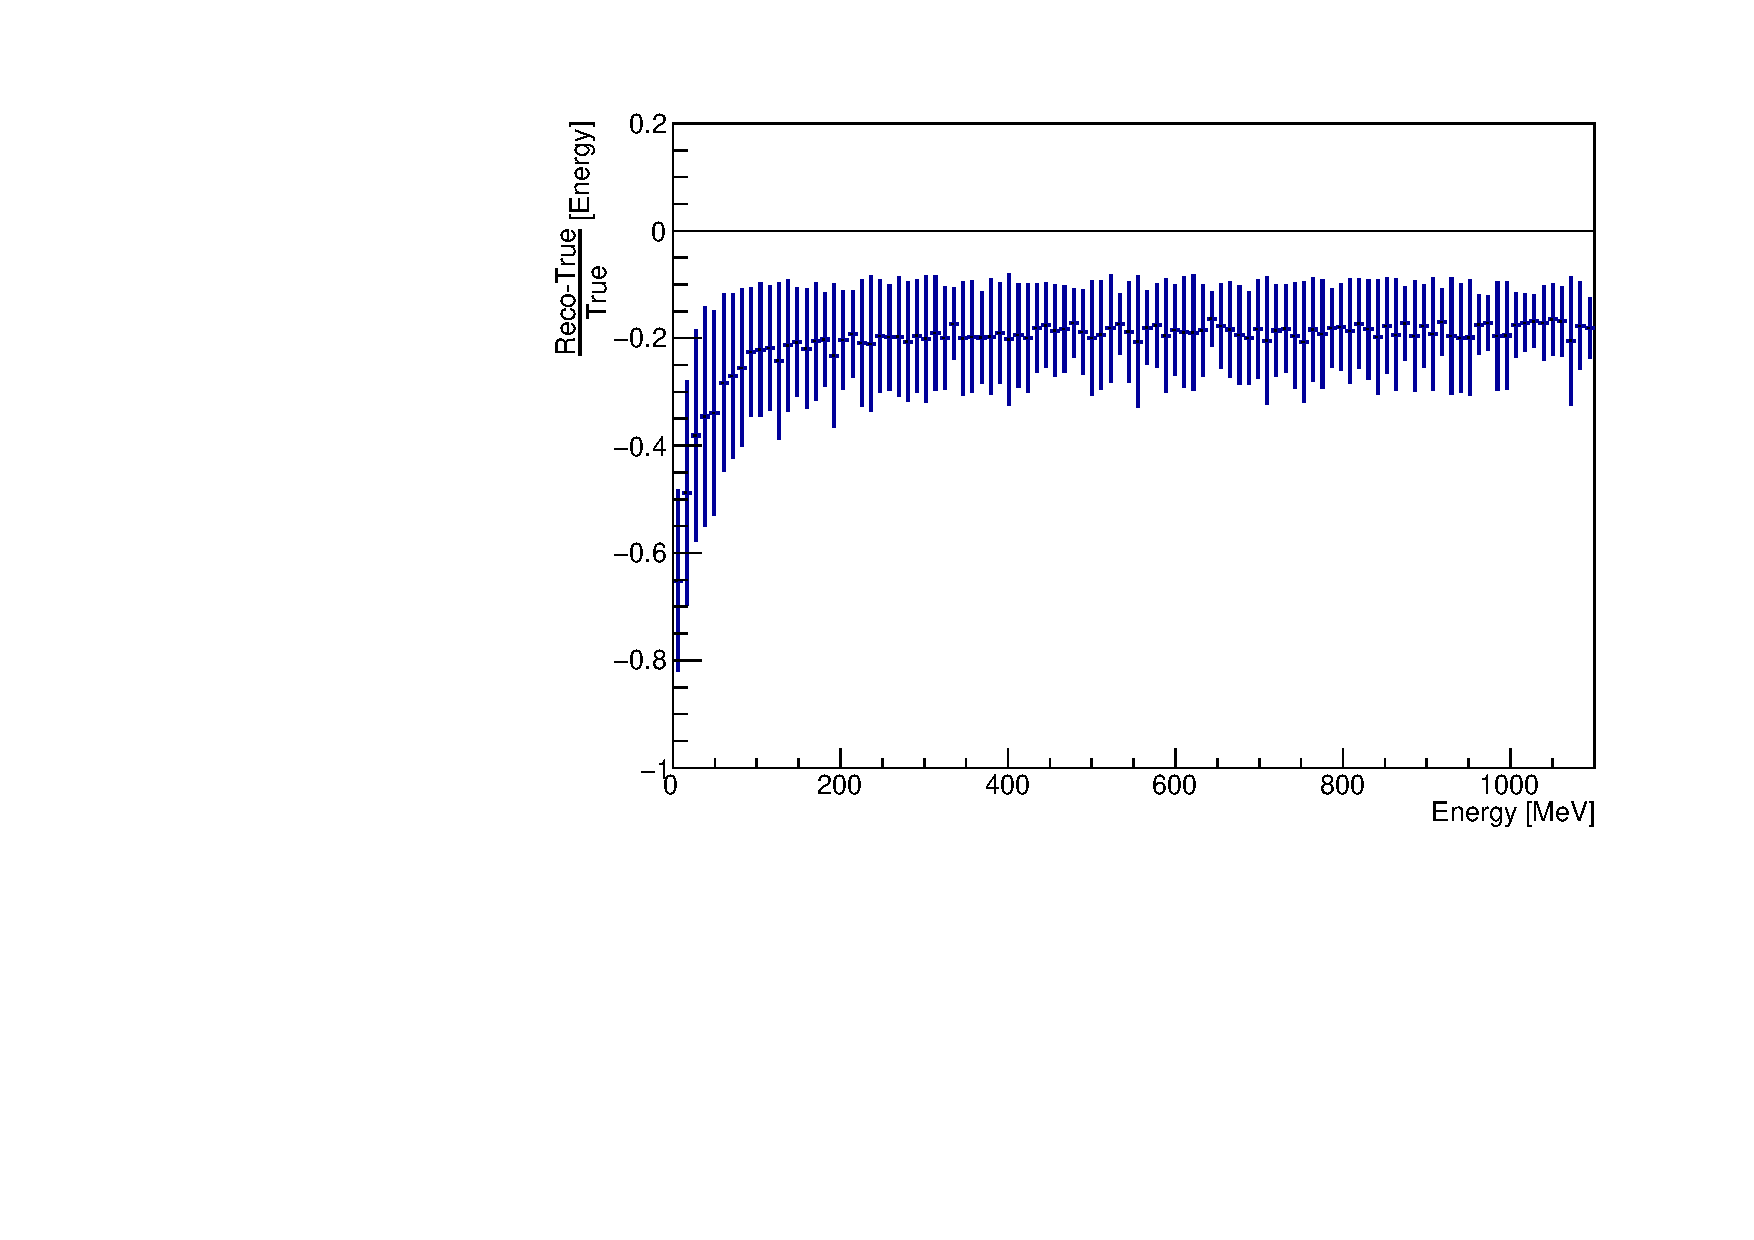
\includegraphics[width = 0.49\textwidth]{figures-chap4/frac_res_vs_energy_cheating_electron_vertex_plane2_ESTAR_showeringE_profile.pdf}
    \caption[Profile histograms of the fractional energy separation as a function of true energy.]{Profile histograms of the fractional energy separation as a function of true energy using the ESTAR method. The profile histograms are constructed from \FigureRef{fig:reconstruction_as_a_function_of_energy} and the y-axis error bars are the standard deviations.  Left: true energy is calculated from the hits. Right: true energy is the energy of the showering electron.}
    \label{fig:reconstruction_as_a_function_of_energy_profile}
\end{figure}



\newpage

\section{Summary of EM Shower Reconstruction}

The \gls{em} shower reconstruction algorithms have been demonstrated to work consistently across all three wire planes in \gls{sbnd} for showers originating from both electrons and photons. The reconstructed energy obtained from the \textit{Shower Linear Energy tool} and the \textit{Shower ESTAR Energy tool} show good agreement with the true energy of $1 \sigma$ width hits with the \textit{Shower ESTAR Energy tool} performing slightly better. The \textit{Shower Num Electrons Energy tool} systematically assigns a slightly higher energy to each of the hits. All three methods underestimate the true energy of the showering particle due to inefficiencies in the hit reconstruction plus the expected presence of an overall bias. The \textit{Shower Num Electrons Energy tool} has the closest agreement with the true energy of the showering particle due to assigning higher energies to the individual hits.

The reconstruction performance is fairly consistent across all shower energies that are expected to be seen by the \gls{bnb}. There is however a slight dip in performance at the lowest energies when compared with the true energy of the showering particle. This is due to a greater percentage of hits having energies below the threshold value. The reconstruction performance also degrades as the angle at which showers are produced to the beamline increases. This is not expected to be much of a concern as the majority of showers will be forward-going. 



\begin{comment}

Why getting dE/dx is hard (page 17).
Using muons as calibration
Energy bias corrections
https://inspirehep.net/files/f10063871db4836eb6ad935fcf761e7d

\end{comment}

